\documentclass[10pt,a4paper]{article}
\usepackage[margin=23mm]{geometry}
\usepackage[T1]{fontenc}
\usepackage{placeins}
\usepackage{lmodern,microtype,amsmath,amssymb,amsthm}
\usepackage{booktabs,tabularx,longtable,array,enumitem,xcolor,hyperref,fancyhdr,titlesec}
\usepackage{graphicx}
\usepackage{tikz}
\usetikzlibrary{arrows.meta,positioning}
\definecolor{ink}{HTML}{18212F}
\definecolor{blue}{HTML}{2457A6}
\definecolor{teal}{HTML}{147D78}
\definecolor{muted}{HTML}{5E6674}
\definecolor{pale}{HTML}{F4F7FA}
\tikzset{
  mapbox/.style={draw=muted!45,rounded corners=2pt,fill=pale,
    text=ink,align=center,font=\small,inner sep=6pt},
  maparrow/.style={-{Stealth[length=2mm]},line width=0.8pt},
  maplabel/.style={font=\footnotesize,align=center,text=ink,fill=white,inner sep=2pt}
}
\hypersetup{colorlinks=true,linkcolor=blue,citecolor=teal,urlcolor=blue,
pdftitle={Circulation-Priced Money: a holding charge that pays for pooled liquidity},
pdfauthor={Siddharth Totla}}
\setlength{\parindent}{1.15em}\setlength{\parskip}{0.13em}
\setlength{\emergencystretch}{1.5em}
\setlist[itemize]{leftmargin=1.5em,itemsep=0.16em,topsep=0.3em}
\setlist[enumerate]{leftmargin=1.6em,itemsep=0.18em,topsep=0.3em}
\renewcommand{\arraystretch}{1.16}
\newcolumntype{L}{>{\raggedright\arraybackslash}X}
\titleformat{\section}{\large\bfseries\color{ink}}{\thesection}{0.55em}{}
\titleformat{\subsection}{\normalsize\bfseries\color{ink}}{\thesubsection}{0.5em}{}
\titlespacing*{\section}{0pt}{1.1em}{0.45em}
\titlespacing*{\subsection}{0pt}{0.8em}{0.3em}
\pagestyle{fancy}\fancyhf{}
\fancyhead[L]{\small\color{muted}Circulation-Priced Money}
\fancyhead[R]{\small\color{muted}Preliminary draft, November 2026}
\fancyfoot[C]{\small\color{muted}\thepage}\renewcommand{\headrulewidth}{0.2pt}
\newtheorem{proposition}{Proposition}
\newtheorem{corollary}{Corollary}
\theoremstyle{remark}
\newtheorem*{remark}{Remark}
\let\savedsection\section
\renewcommand{\section}{\FloatBarrier\savedsection}
% A value or statement that waits for the final map or for a check; it prints in colour so none can be missed.
\newcommand{\pending}[1]{\textcolor{red!70!black}{[#1]}}
% Sums over the cycle (the last two completed months) carry a hat.
\newcommand{\cyc}[1]{\widehat{#1}}
% Numbers quoted in the paper, one macro each. WRITTEN BY scripts/paper_numbers.py: do not edit by hand.
% Results folder: confirmation_quote
% Source files as the run hashed them (sha256):
%   scripts/run_economy_figures.py: 340602c51e81dafab57eef35b7b8b5881db72b3de8f95bc5fda2a920a790b820
%   scripts/run_economy_population.py: d8a5b67db2e2c4f33d891e6c5f712af304777cfd908e853808c0ac0dddef1840
%   src/cpm_abm/comet.py: 05435046e350c88e45ee717b8e018c461572fb8f4cbc636ad945d7aa8688e6ed
%   src/cpm_abm/core_model.py: f040e3abe79bc3ea8fa7aaaa90b296aff275ab354940777e02e1570dd206ac29
%   src/cpm_abm/economy_abm.py: 314e5a790bb189bb378a74433318555e0b509203e37f0416e9d2fffe5c30e258
%   src/cpm_abm/engine/__init__.py: 308f9b6b99f7d4c1010024f1fcf3323dd6e18c98f4e82d52a2fa5cdf4b758601
%   src/cpm_abm/engine/constants.py: 65e3647eeb0e0fc4bd1a20c65383de1d08a9379a1226e6ff9f39f9969119cfd5
%   src/cpm_abm/engine/ledger.py: 90f0d2c9eb3ac2350a8e21b63400e093f841047e473733ad285a0810f87b4586
%   src/cpm_abm/engine/lending_rules.py: 390b9bf22453c9a24afa463f7781dbf6eefff46a2fbdc7d64fd2ae249c7dfd3a
%   src/cpm_abm/engine/measures.py: 71e51f755042d6cdec6fa9b85519e7d643795ea8bb6e938691ef2e41d7ac484c
%   src/cpm_abm/engine/network.py: a8103f7960ec1acc384c65cd8ff57cf3ba221890be88907d8ae55a28c3b59ea1
%   src/cpm_abm/engine/population.py: f0935a22cbc6d313a96d716144fde95d63721b749a630520deb6810822c8b44c
%   src/cpm_abm/engine/rates.py: 3a3bca303474c1980bce169dc10ae469f3e3bebe8e68403cf0933db0ad087514
%   src/cpm_abm/engine/settings.py: 45f9043438915d4609508ddbd69516db03d785cb53c77f76314be6de2bab9b2a
%   src/cpm_abm/engine/world.py: 94efac59446e5932c04e653a13a766337713850fd90818cafa4df054b074f069
%   src/cpm_abm/engine/world_close.py: 8ac0e39fa3ae0b612c7eefe782ee32b7681cb0ffadcadae5b005718703e3f596
%   src/cpm_abm/engine/world_credit.py: 510179d18ae0f20023dd594a63059594c644deb9f3d2e6f607875e0c88e5c2ef
%   src/cpm_abm/engine/world_day.py: 655d650b181f9d5bf95dee2e7308122262698c64d390929602e6072bddaf88e2
%   src/cpm_abm/engine/world_dealing.py: 76d119a5cd1cb79cbb74bb38b2c51616e5014b724378f64d2861b944c9bfdc87
%   src/cpm_abm/engine/world_month.py: 3e566861eb579ee69ea7fc7a706bc9eec47bd5afb61ee173ce720e510bdf15dd
%   src/cpm_abm/engine/world_payments.py: 5097b263bbced73f388f8e4d76e83a31adc9101d3cf0be20e152d5a6dfacadee
%   src/cpm_abm/engine/world_state.py: f3d2446965ca1ca70e10103bf2b824937433237797915a893b108280c5f49596
%   src/cpm_abm/experiment/__init__.py: 5f3e62ebf37ff7a0306e4006d36d10460c83b726c43e85d254fc1ee6b0cf5275
%   src/cpm_abm/experiment/accounts.py: 1f74fc9d93845543231125b5dd4b9e81c2785dbd9463b9cc06fcde382902e44e
%   src/cpm_abm/experiment/claims.py: ec9e1802cd13f8c936a0c5e9cdf7ddf71aed14d756c6e55e1b5539f7c8901c47
%   src/cpm_abm/experiment/gains.py: 4ff21c34d30d1af339f489958610b3419462f8bdbaa04ba2c4be2ad630733826
%   src/cpm_abm/experiment/grid.py: 0ea65186e1fdf0f95086c89389cd65b7c1afc5140ebfe4ad1632fdcc99397ea0
%   src/cpm_abm/experiment/jobs.py: 5d1affeced306b3c62cd87b23316fcbd34dd3c938e3806c0b8a69b3c2ef34965
%   src/cpm_abm/experiment/notes.py: bc9ea00b22d4685f854219c099c82110fe474787ef3998a1ee401ff44d046654
%   src/cpm_abm/experiment/region.py: 45b41daeb40ff392601b572ca351a14b7bd529518e6a470a9b8337d3ae6caa2b
%   src/cpm_abm/experiment/statistics.py: 501d69536c71074a5100a516cd8a5a905e26e4b26269d0f21e0aa7f31acc6ae5
%   src/cpm_abm/experiment/store.py: 204c5fb32068f3739260f06c42f44c8b144acd7373f1ae14e9fb125a2da5f772
% Seed set: confirmation, 30 seeds: 20261401, 20261402, 20261403, 20261404, 20261405, 20261406, 20261407, 20261408, 20261409, 20261410, 20261411, 20261412, 20261413, 20261414, 20261415, 20261416, 20261417, 20261418, 20261419, 20261420, 20261421, 20261422, 20261423, 20261424, 20261425, 20261426, 20261427, 20261428, 20261429, 20261430
% Population: 4000 people
% Side checks, bounds, robustness sets and the seed plan are read beside: development_map (seed set development, 3 seeds)
% A macro reading \textbf{??} is a number this result does not store; numbers_report.txt says which.
\newcommand{\NumPeople}{4{,}000}
\newcommand{\NumSeeds}{30}
\newcommand{\NumSeedsDev}{3}
\newcommand{\FailBanks}{3.585\% to 3.691\%}
\newcommand{\FailBanksLow}{3.585\%}
\newcommand{\FailBanksHigh}{3.691\%}
\newcommand{\FailDefiLow}{3.264\%}
\newcommand{\FailDefiHigh}{3.630\%}
\newcommand{\FailCpmLow}{1.826\%}
\newcommand{\FailCpmHigh}{2.997\%}
\newcommand{\FailBanksStress}{5.757\% to 6.058\%}
\newcommand{\FailBanksStressLow}{5.757\%}
\newcommand{\FailBanksStressHigh}{6.058\%}
\newcommand{\FailCpmStressLow}{4.204\%}
\newcommand{\FailCpmStressHigh}{6.773\%}
\newcommand{\ChargeLow}{0.062\%}
\newcommand{\ChargeHigh}{0.179\%}
\newcommand{\RunAdoption}{20\%}
\newcommand{\FailBanksMean}{3.6\%}
\newcommand{\FailDefiMean}{3.5\%}
\newcommand{\FailPoolMean}{2.5\%}
\newcommand{\FailCpmMean}{2.4\%}
\newcommand{\FailBanksStressMean}{5.9\%}
\newcommand{\FailDefiStressMean}{5.7\%}
\newcommand{\FailCpmStressMean}{4.9\%}
\newcommand{\GainBanksMedian}{\$262}
\newcommand{\GainBanksFaceMedian}{\$550}
\newcommand{\GainDefiMedian}{\$140}
\newcommand{\GainDefiFaceMedian}{\$429}
\newcommand{\GainBanksBoundLow}{\$59}
\newcommand{\GainDefiBoundLow}{\$29}
\newcommand{\RealCostBanksLow}{\$4.7}
\newcommand{\RealCostDefiLow}{$-$\$2.0}
\newcommand{\RealCostDefiHigh}{\$0.2}
\newcommand{\RescueEvenDefiLow}{\$1.59}
\newcommand{\RescueEvenDefiMedian}{\$1.96}
\newcommand{\RescueEvenDefiHigh}{\$2.06}
\newcommand{\RescueEvenBanksLow}{\$4.76}
\newcommand{\RescueEvenBanksMedian}{\$6.58}
\newcommand{\RescueEvenBanksHigh}{\$9.14}
\newcommand{\CentsCompletedBanks}{0.584}
\newcommand{\CentsCompletedDefi}{0.521}
\newcommand{\CentsCompletedCpm}{0.516}
\newcommand{\ShareBehindBanks}{10.6\%}
\newcommand{\ShareBehindDefi}{13.2\%}
\newcommand{\ShareBehindBanksMoney}{16.8\%}
\newcommand{\ShareBehindDefiMoney}{19.0\%}
\newcommand{\PersonMedianBanks}{\$116}
\newcommand{\PersonMedianDefi}{\$63}
\newcommand{\PersonFifthBanks}{$-$\$103}
\newcommand{\PersonFifthDefi}{$-$\$90}
\newcommand{\ChargeFrom}{0.06\%}
\newcommand{\ChargeTo}{0.18\%}
\newcommand{\BridgePriceCpm}{2.1\%}
\newcommand{\BridgePricePoolLow}{4.3\%}
\newcommand{\BridgePricePoolHigh}{8.4\%}
\newcommand{\CellsNoDistress}{21}
\newcommand{\StableAsBuilt}{21}
\newcommand{\StableBoth}{20}
\newcommand{\CellsAll}{105}
\newcommand{\CellsGainPositive}{105}
\newcommand{\CellsFewerFailures}{99}
\newcommand{\ChargeDollars}{\$4.7}
\newcommand{\PoolBridgingPool}{\$2{,}645}
\newcommand{\PoolBridgingCpm}{\$2{,}982}
\newcommand{\RevolvedPool}{\$706}
\newcommand{\RevolvedCpm}{\$637}
\newcommand{\FailedDollarsPool}{\$2{,}147}
\newcommand{\FailedDollarsCpm}{\$2{,}094}
\newcommand{\StandbyPool}{\$31}
\newcommand{\StandbyCpm}{\$50}
\newcommand{\PrecautionBanks}{0.46}
\newcommand{\PrecautionDefi}{0.54}
\newcommand{\PrecautionPool}{0.36}
\newcommand{\PrecautionCpm}{0.36}
\newcommand{\GainOverPool}{\$15}
\newcommand{\StandbyChange}{59\%}
\newcommand{\PoolBridgingChange}{13\%}
\newcommand{\RevolvedChange}{10\%}
\newcommand{\GainOverPoolLate}{\$17}
\newcommand{\GainPerChargeDollar}{3.6}
\newcommand{\OwnersMedianWorst}{0.02}
\newcommand{\OwnersTenthLeast}{0.31}
\newcommand{\OwnersTenthWorst}{0.52}
\newcommand{\SeedsPlanned}{26}
\newcommand{\SeedsAssured}{30}
\newcommand{\SpreadBinding}{1.1658}
\newcommand{\FreedomBinding}{42}
\newcommand{\SpreadBindingBound}{1.293}
\newcommand{\SeedsCellMost}{27}
\newcommand{\CellsUnderpowered}{no}
\newcommand{\SeedsConfirm}{30}
\newcommand{\SeedsExtended}{60}
\newcommand{\SeedAssurance}{0.8}
\newcommand{\WilsonConfirm}{21}
\newcommand{\WilsonConfirmBonf}{24}
\newcommand{\WilsonConfirmBonfIndexed}{23}
\newcommand{\WilsonExtended}{38}
\newcommand{\WilsonExtendedBonf}{42}
\newcommand{\WilsonExtendedBonfIndexed}{42}
\newcommand{\SpreadResolved}{\$2.59}
\newcommand{\RegionCellsZero}{19}
\newcommand{\RegionCellsHalf}{14}
\newcommand{\RegionCellsOne}{13}
\newcommand{\RegionCellsOneHalf}{10}
\newcommand{\RegionCellsTwo}{4}
\newcommand{\ClaimCellsAsBuilt}{20}
\newcommand{\ClaimCellsBoth}{19}
\newcommand{\ClaimCellsFalsified}{no}
\newcommand{\ClaimCellsUnderpowered}{no}
\newcommand{\ClaimHoldsSomewhere}{17}
\newcommand{\ClaimSeedsPlanned}{14}
\newcommand{\ClaimSeedsCellMost}{13}
\newcommand{\IndexedRegionZero}{14}
\newcommand{\IndexedRegionHalf}{13}
\newcommand{\IndexedRegionOne}{12}
\newcommand{\IndexedRegionOneHalf}{10}
\newcommand{\IndexedRegionTwo}{4}
\newcommand{\IndexedValid}{14}
\newcommand{\IndexedHolds}{14}
\newcommand{\IndexedGainBanks}{\$342}
\newcommand{\IndexedGainDefi}{\$155}
\newcommand{\IndexedCpmGainBanks}{\$343}
\newcommand{\IndexedCpmGainDefi}{\$156}
\newcommand{\GroupLowDefiFace}{\$136}
\newcommand{\GroupLowDefiFaceBound}{\$119}
\newcommand{\GroupLowBanksZero}{\$0.5}
\newcommand{\GroupLowBanksZeroBound}{$-$\$2.6}
\newcommand{\SeedsPersistentLeast}{26}
\newcommand{\GainBanksShared}{\$246}
\newcommand{\LenderShareZeroBanks}{1.88}
\newcommand{\GainDefiShared}{\$125}
\newcommand{\LenderShareZeroDefi}{0.98}
\newcommand{\HoldingDaysCpm}{26.9}
\newcommand{\HoldingDaysPool}{27.2}
\newcommand{\VelocityBanks}{10.32}
\newcommand{\VelocityDefi}{10.64}
\newcommand{\VelocityPool}{12.48}
\newcommand{\VelocityCpm}{12.54}
\newcommand{\RobustBaseSurviveBanks}{7}
\newcommand{\RobustBaseSurviveDefi}{7}
\newcommand{\RobustBasePartFive}{0.45}
\newcommand{\RobustMeasuredSurviveBanks}{7}
\newcommand{\RobustMeasuredSurviveDefi}{7}
\newcommand{\RobustMeasuredPartFive}{0.78}
\newcommand{\RobustThresholdTenSurviveBanks}{7}
\newcommand{\RobustThresholdTenSurviveDefi}{7}
\newcommand{\RobustThresholdTenPartFive}{0.84}
\newcommand{\RobustThresholdTenCriticalMass}{5\%}
\newcommand{\RobustThresholdTwentySurviveBanks}{7}
\newcommand{\RobustThresholdTwentySurviveDefi}{7}
\newcommand{\RobustThresholdTwentyPartFive}{0.54}
\newcommand{\RobustThresholdTwentyCriticalMass}{5\%}
\newcommand{\RobustThresholdThirtySurviveBanks}{7}
\newcommand{\RobustThresholdThirtySurviveDefi}{7}
\newcommand{\RobustThresholdThirtyPartFive}{0.18}
\newcommand{\RobustThresholdThirtyCriticalMass}{5\%}
\newcommand{\RobustRingSurviveBanks}{7}
\newcommand{\RobustRingSurviveDefi}{7}
\newcommand{\RobustRingPartFive}{0.44}
\newcommand{\RobustRingNeighbourhoodSurviveBanks}{7}
\newcommand{\RobustRingNeighbourhoodSurviveDefi}{7}
\newcommand{\RobustRingNeighbourhoodPartFive}{0.35}
\newcommand{\RobustRingThresholdSurviveBanks}{7}
\newcommand{\RobustRingThresholdSurviveDefi}{7}
\newcommand{\RobustRingThresholdPartFive}{0.58}
\newcommand{\RobustRingThresholdCriticalMass}{5\%}
\newcommand{\RobustRingThresholdNeighbourhoodSurviveBanks}{7}
\newcommand{\RobustRingThresholdNeighbourhoodSurviveDefi}{7}
\newcommand{\RobustRingThresholdNeighbourhoodPartFive}{0.39}
\newcommand{\RobustRingThresholdNeighbourhoodCriticalMass}{5\%}
\newcommand{\RobustRingLocalSurviveBanks}{7}
\newcommand{\RobustRingLocalSurviveDefi}{7}
\newcommand{\RobustRingLocalPartFive}{0.44}
\newcommand{\RobustRingLocalThresholdNeighbourhoodSurviveBanks}{7}
\newcommand{\RobustRingLocalThresholdNeighbourhoodSurviveDefi}{7}
\newcommand{\RobustRingLocalThresholdNeighbourhoodPartFive}{0.50}
\newcommand{\RobustRingLocalThresholdNeighbourhoodCriticalMass}{5\%}
\newcommand{\RobustHubsSurviveBanks}{7}
\newcommand{\RobustHubsSurviveDefi}{7}
\newcommand{\RobustHubsPartFive}{0.45}
\newcommand{\RobustHubsLargestSurviveBanks}{7}
\newcommand{\RobustHubsLargestSurviveDefi}{7}
\newcommand{\RobustHubsLargestPartFive}{0.58}
\newcommand{\RobustHubsMeasuredSurviveBanks}{7}
\newcommand{\RobustHubsMeasuredSurviveDefi}{7}
\newcommand{\RobustHubsMeasuredPartFive}{0.78}
\newcommand{\RobustHubsMeasuredLargestSurviveBanks}{7}
\newcommand{\RobustHubsMeasuredLargestSurviveDefi}{7}
\newcommand{\RobustHubsMeasuredLargestPartFive}{0.82}
\newcommand{\RobustStressBaseCells}{7}
\newcommand{\RobustStressBaseFailCpm}{4.27\%}
\newcommand{\RobustStressBaseFailBanks}{5.70\%}
\newcommand{\RobustStressBaseFailDefi}{5.41\%}
\newcommand{\RobustStressBaseFewer}{7}
\newcommand{\RobustStressBaseGainPositive}{7}
\newcommand{\RobustStressBaseServedHigh}{0.41}
\newcommand{\RobustStressRingCells}{7}
\newcommand{\RobustStressRingFailCpm}{4.17\%}
\newcommand{\RobustStressRingFailBanks}{5.77\%}
\newcommand{\RobustStressRingFailDefi}{5.50\%}
\newcommand{\RobustStressRingFewer}{7}
\newcommand{\RobustStressRingGainPositive}{7}
\newcommand{\RobustStressRingServedHigh}{0.43}
\newcommand{\RobustStressHubsCells}{7}
\newcommand{\RobustStressHubsFailCpm}{5.35\%}
\newcommand{\RobustStressHubsFailBanks}{7.28\%}
\newcommand{\RobustStressHubsFailDefi}{6.95\%}
\newcommand{\RobustStressHubsFewer}{7}
\newcommand{\RobustStressHubsGainPositive}{7}
\newcommand{\RobustStressHubsServedHigh}{0.42}
\newcommand{\RuleCheckGapMean}{0.125}
\newcommand{\RuleCheckGapFirstSeed}{0.128}
\newcommand{\RuleCheckGapSecondSeed}{0.126}
\newcommand{\RuleCheckGapThirdSeed}{0.122}
\newcommand{\KnockOnBanks}{0.57\%}
\newcommand{\KnockOnCpm}{0.41\%}
\newcommand{\KnockOnGap}{$-$0.16\%}
\newcommand{\KnockOnGapRange}{$-$0.22\% to $-$0.03\%}
\newcommand{\ManyKnockOnBanks}{0.0\%}
\newcommand{\ManyKnockOnPool}{10.5\%}
\newcommand{\ManyKnockOnCpm}{5.7\%}
\newcommand{\KnockOnBanksStress}{0.84\%}
\newcommand{\KnockOnCpmStress}{0.69\%}
\newcommand{\KnockOnGapStress}{$-$0.14\%}
\newcommand{\KnockOnGapStressRange}{$-$0.42\% to 0.15\%}
\newcommand{\ManyKnockOnBanksStress}{0.0\%}
\newcommand{\ManyKnockOnPoolStress}{17.8\%}
\newcommand{\ManyKnockOnCpmStress}{13.2\%}
\newcommand{\NettingShareMost}{0.000\%}
\newcommand{\BoundaryTwenty}{none up to 2 points}
\newcommand{\BoundaryThirty}{none up to 2 points}
\newcommand{\BoundaryFortyFive}{1.8 points}
\newcommand{\BoundaryRepeatValues}{116{,}325}
\newcommand{\BoundaryRepeatDiffer}{0}
\newcommand{\ReadFirstRegion}{19}
\newcommand{\ReadFirstPersistentLow}{26}
\newcommand{\ReadFirstPersistentHigh}{30}
\newcommand{\ReadFirstCapital}{0.97}
\newcommand{\ReadFirstServedCpm}{0.84}
\newcommand{\ReadFirstServedPool}{0.77}
\newcommand{\ReadFirstPriceCpm}{2.1\%}
\newcommand{\ReadFirstPricePool}{6.7\%}
\newcommand{\ReadFirstFailBanks}{3.65\%}
\newcommand{\ReadFirstFailPool}{2.59\%}
\newcommand{\ReadFirstFailCpm}{2.51\%}
\newcommand{\ReadFirstGainBanks}{\$262}
\newcommand{\ReadFirstGainDefi}{\$140}
\newcommand{\ReadFirstGainOverPool}{\$15}
\newcommand{\ReadFirstGainPositive}{105}
\newcommand{\ReadFirstFewerFailures}{99}
\newcommand{\ReadSecondRegion}{2}
\newcommand{\ReadSecondPersistentLow}{6}
\newcommand{\ReadSecondPersistentHigh}{23}
\newcommand{\ReadSecondCapital}{0.77}
\newcommand{\ReadSecondServedCpm}{0.52}
\newcommand{\ReadSecondServedPool}{0.17}
\newcommand{\ReadSecondPriceCpm}{2.4\%}
\newcommand{\ReadSecondPricePool}{11.4\%}
\newcommand{\ReadSecondFailBanks}{3.65\%}
\newcommand{\ReadSecondFailPool}{3.35\%}
\newcommand{\ReadSecondFailCpm}{2.86\%}
\newcommand{\ReadSecondGainBanks}{\$217}
\newcommand{\ReadSecondGainDefi}{\$90}
\newcommand{\ReadSecondGainOverPool}{\$61}
\newcommand{\ReadSecondGainPositive}{105}
\newcommand{\ReadSecondFewerFailures}{98}
\newcommand{\ReadSecondGainBanksLower}{17\%}
\newcommand{\ReadSecondGainDefiLower}{35\%}
\newcommand{\ReadSecondRegionTwo}{0}
\newcommand{\PathFirstRatioOne}{1.01}
\newcommand{\PathFirstCapitalOne}{\$293}
\newcommand{\PathFirstTargetOne}{\$292}
\newcommand{\PathFirstServedOne}{0.87}
\newcommand{\PathFirstRatioTwo}{1.00}
\newcommand{\PathFirstCapitalTwo}{\$614}
\newcommand{\PathFirstTargetTwo}{\$611}
\newcommand{\PathFirstServedTwo}{0.90}
\newcommand{\PathFirstRatioThree}{1.00}
\newcommand{\PathFirstCapitalThree}{\$899}
\newcommand{\PathFirstTargetThree}{\$895}
\newcommand{\PathFirstServedThree}{0.90}
\newcommand{\PathFirstRatioFour}{1.00}
\newcommand{\PathFirstCapitalFour}{\$1{,}284}
\newcommand{\PathFirstTargetFour}{\$1{,}286}
\newcommand{\PathFirstServedFour}{0.88}
\newcommand{\PathFirstRatioFive}{0.96}
\newcommand{\PathFirstCapitalFive}{\$1{,}653}
\newcommand{\PathFirstTargetFive}{\$1{,}728}
\newcommand{\PathFirstServedFive}{0.80}
\newcommand{\PathSecondRatioOne}{0.97}
\newcommand{\PathSecondCapitalOne}{\$287}
\newcommand{\PathSecondTargetOne}{\$298}
\newcommand{\PathSecondServedOne}{0.81}
\newcommand{\PathSecondRatioTwo}{0.91}
\newcommand{\PathSecondCapitalTwo}{\$563}
\newcommand{\PathSecondTargetTwo}{\$630}
\newcommand{\PathSecondServedTwo}{0.72}
\newcommand{\PathSecondRatioThree}{0.91}
\newcommand{\PathSecondCapitalThree}{\$792}
\newcommand{\PathSecondTargetThree}{\$884}
\newcommand{\PathSecondServedThree}{0.70}
\newcommand{\PathSecondRatioFour}{0.85}
\newcommand{\PathSecondCapitalFour}{\$1{,}040}
\newcommand{\PathSecondTargetFour}{\$1{,}241}
\newcommand{\PathSecondServedFour}{0.59}
\newcommand{\PathSecondRatioFive}{0.75}
\newcommand{\PathSecondCapitalFive}{\$1{,}152}
\newcommand{\PathSecondTargetFive}{\$1{,}564}
\newcommand{\PathSecondServedFive}{0.43}
\newcommand{\CutPassZeroTwoFive}{4}
\newcommand{\CutPassZeroThree}{5}
\newcommand{\CutPassZeroThreeFive}{7}
\newcommand{\CutPassHalfTwoFive}{2}
\newcommand{\CutPassHalfThree}{4}
\newcommand{\CutPassHalfThreeFive}{6}
\newcommand{\CutPassOneTwoFive}{0}
\newcommand{\CutPassOneThree}{2}
\newcommand{\CutPassOneThreeFive}{5}
\newcommand{\CutPassOneHalfTwoFive}{0}
\newcommand{\CutPassOneHalfThree}{0}
\newcommand{\CutPassOneHalfThreeFive}{4}
\newcommand{\CutPassTwoTwoFive}{0}
\newcommand{\CutPassTwoThree}{0}
\newcommand{\CutPassTwoThreeFive}{1}
\newcommand{\CutSeeds}{26}
\newcommand{\CutSeedsAside}{4}
\newcommand{\CutSeedsTried}{30}
\newcommand{\CutCells}{105}
\newcommand{\CutGainPositive}{105}
\newcommand{\CutFewerFailures}{98}
\newcommand{\SpiralCostSourced}{\$0.18}
\newcommand{\SpiralCostTen}{\$1.79}
\newcommand{\SpiralCostHundred}{\$18}
\newcommand{\SpiralCostThousand}{\$179}
\newcommand{\ExploreSeeds}{3}
\newcommand{\ExploreBaseDefiLow}{\$60}
\newcommand{\ExploreBaseDefiHigh}{\$217}
\newcommand{\ExploreCustodyDefiLow}{\$53}
\newcommand{\ExploreCustodyDefiHigh}{\$192}
\newcommand{\ExploreShockEarlyFailLow}{4.86\%}
\newcommand{\ExploreShockEarlyFailHigh}{5.51\%}
\newcommand{\ExploreShockEarlyBanksLow}{6.26\%}
\newcommand{\ExploreShockEarlyBanksHigh}{6.26\%}
\newcommand{\ExploreShockLateFailLow}{3.62\%}
\newcommand{\ExploreShockLateFailHigh}{3.95\%}
\newcommand{\ExploreShockLateBanksLow}{5.04\%}
\newcommand{\ExploreShockLateBanksHigh}{5.04\%}
\newcommand{\GainAfterBanksPositive}{105}
\newcommand{\GainAfterBanksBehind}{0}
\newcommand{\GainAfterBanksLow}{\$20}
\newcommand{\GainAfterBanksMedianZero}{\$313}
\newcommand{\GainAfterBanksMedianTwo}{\$271}
\newcommand{\GainAfterBanksLowerTwo}{14\%}
\newcommand{\GainAfterDefiPositive}{101}
\newcommand{\GainAfterDefiBehind}{4}
\newcommand{\GainAfterDefiLow}{$-$\$61}
\newcommand{\GainAfterDefiMedianZero}{\$163}
\newcommand{\GainAfterDefiMedianTwo}{\$129}
\newcommand{\GainAfterDefiLowerTwo}{21\%}
\newcommand{\FailedWageShareBanks}{61\%}
\newcommand{\NoCardFailedShareBanks}{65\%}
\newcommand{\FailedValueBanks}{\$2{,}806}
\newcommand{\NoCardPeople}{16.1\%}
\newcommand{\FailedWageShareCpm}{61\%}
\newcommand{\NoCardFailedShareCpm}{62\%}
\newcommand{\FailedValueCpm}{\$2{,}011}
\newcommand{\FailCutBanks}{35\%}
\newcommand{\FailCutDefi}{33\%}
\newcommand{\FailCutPoolBanks}{33\%}
\newcommand{\FailCutBanksStress}{17\%}
\newcommand{\FailCutDefiStress}{13\%}
\newcommand{\OutsidePaidBanks}{\$1{,}043}
\newcommand{\OutsidePaidDefi}{\$817}
\newcommand{\OutsidePaidCpm}{\$649}
\newcommand{\OutsideCutBanks}{34\%}
\newcommand{\OutsideCutBanksLow}{11\%}
\newcommand{\OutsideCutBanksHigh}{61\%}
\newcommand{\OutsideCutDefi}{21\%}
\newcommand{\OutsideCashCutBanks}{26\%}
\newcommand{\BridgeCutLow}{52\%}
\newcommand{\BridgeCutHigh}{75\%}
\newcommand{\GainBanksSpending}{0.34\%}
\newcommand{\GainDefiSpending}{0.18\%}
\newcommand{\GainBanksFaceSpending}{0.71\%}
\newcommand{\GainDefiFaceSpending}{0.56\%}
\newcommand{\PersonMedianBanksSpending}{0.15\%}
\newcommand{\PersonMedianDefiSpending}{0.08\%}
\newcommand{\GainAfterSecondBanksPositive}{105}
\newcommand{\GainAfterSecondBanksBehind}{0}
\newcommand{\GainAfterSecondBanksLow}{\$48}
\newcommand{\GainAfterSecondBanksMedianZero}{\$275}
\newcommand{\GainAfterSecondBanksMedianTwo}{\$174}
\newcommand{\GainAfterSecondBanksLowerTwo}{37\%}
\newcommand{\GainAfterSecondDefiPositive}{102}
\newcommand{\GainAfterSecondDefiBehind}{3}
\newcommand{\GainAfterSecondDefiLow}{$-$\$18}
\newcommand{\GainAfterSecondDefiMedianZero}{\$111}
\newcommand{\GainAfterSecondDefiMedianTwo}{\$65}
\newcommand{\GainAfterSecondDefiLowerTwo}{42\%}
\newcommand{\SourceYieldTwo}{\$55}
\newcommand{\SourceYieldFourFour}{\$138}
\newcommand{\SourceYieldSix}{\$194}
\newcommand{\SourceInterestTwo}{\$102}
\newcommand{\SourceInterestFourFour}{\$118}
\newcommand{\SourceInterestSix}{\$133}
\newcommand{\SourceCardTwo}{\$41}
\newcommand{\SourceCardFourFour}{\$42}
\newcommand{\SourceCardSix}{\$42}
\newcommand{\SourceFeesTwo}{\$34}
\newcommand{\SourceFeesFourFour}{\$65}
\newcommand{\SourceFeesSix}{\$69}
\newcommand{\SourcePoolTwo}{$-$\$22}
\newcommand{\SourcePoolFourFour}{$-$\$17}
\newcommand{\SourcePoolSix}{$-$\$17}
\newcommand{\SourceSavingsTwo}{$-$\$22}
\newcommand{\SourceSavingsFourFour}{$-$\$35}
\newcommand{\SourceSavingsSix}{$-$\$43}
\newcommand{\SourceOtherTwo}{$-$\$1.8}
\newcommand{\SourceOtherFourFour}{$-$\$1.6}
\newcommand{\SourceOtherSix}{$-$\$1.6}
\newcommand{\SourceTotalTwo}{\$197}
\newcommand{\SourceTotalFourFour}{\$309}
\newcommand{\SourceTotalSix}{\$376}
\newcommand{\SourceYieldShareTwo}{28\%}
\newcommand{\SourceYieldShareFourFour}{45\%}
\newcommand{\SourceYieldShareSix}{52\%}
\newcommand{\SourceInterestShareTwo}{52\%}
\newcommand{\SourceInterestShareFourFour}{38\%}
\newcommand{\SourceInterestShareSix}{35\%}
\newcommand{\ChargeGainFirstMedianZero}{\$15}
\newcommand{\ChargeGainFirstLowZero}{\$4.9}
\newcommand{\ChargeGainFirstAboveZero}{21}
\newcommand{\ChargeGainFirstFewerZero}{21}
\newcommand{\ChargeGainFirstMedianHalf}{\$15}
\newcommand{\ChargeGainFirstLowHalf}{\$4.7}
\newcommand{\ChargeGainFirstAboveHalf}{21}
\newcommand{\ChargeGainFirstFewerHalf}{21}
\newcommand{\ChargeGainFirstMedianOne}{\$13}
\newcommand{\ChargeGainFirstLowOne}{\$4.6}
\newcommand{\ChargeGainFirstAboveOne}{21}
\newcommand{\ChargeGainFirstFewerOne}{19}
\newcommand{\ChargeGainFirstMedianOneHalf}{\$13}
\newcommand{\ChargeGainFirstLowOneHalf}{\$3.8}
\newcommand{\ChargeGainFirstAboveOneHalf}{21}
\newcommand{\ChargeGainFirstFewerOneHalf}{18}
\newcommand{\ChargeGainFirstMedianTwo}{\$12}
\newcommand{\ChargeGainFirstLowTwo}{\$0.1}
\newcommand{\ChargeGainFirstAboveTwo}{21}
\newcommand{\ChargeGainFirstFewerTwo}{18}
\newcommand{\ChargeGainFirstAboveAll}{105}
\newcommand{\ChargeGainFirstFewerAll}{97}
\newcommand{\ChargeGainFirstCells}{105}
\newcommand{\ChargeGainSecondMedianZero}{\$61}
\newcommand{\ChargeGainSecondLowZero}{\$34}
\newcommand{\ChargeGainSecondAboveZero}{21}
\newcommand{\ChargeGainSecondFewerZero}{21}
\newcommand{\ChargeGainSecondMedianHalf}{\$56}
\newcommand{\ChargeGainSecondLowHalf}{\$35}
\newcommand{\ChargeGainSecondAboveHalf}{21}
\newcommand{\ChargeGainSecondFewerHalf}{21}
\newcommand{\ChargeGainSecondMedianOne}{\$53}
\newcommand{\ChargeGainSecondLowOne}{\$32}
\newcommand{\ChargeGainSecondAboveOne}{21}
\newcommand{\ChargeGainSecondFewerOne}{19}
\newcommand{\ChargeGainSecondMedianOneHalf}{\$50}
\newcommand{\ChargeGainSecondLowOneHalf}{\$27}
\newcommand{\ChargeGainSecondAboveOneHalf}{21}
\newcommand{\ChargeGainSecondFewerOneHalf}{18}
\newcommand{\ChargeGainSecondMedianTwo}{\$46}
\newcommand{\ChargeGainSecondLowTwo}{\$21}
\newcommand{\ChargeGainSecondAboveTwo}{21}
\newcommand{\ChargeGainSecondFewerTwo}{15}
\newcommand{\ChargeGainSecondAboveAll}{105}
\newcommand{\ChargeGainSecondFewerAll}{94}
\newcommand{\ChargeGainSecondCells}{105}
\newcommand{\LendCouponTwo}{4.39\%}
\newcommand{\LendCouponTwoFive}{4.90\%}
\newcommand{\LendCouponThree}{5.42\%}
\newcommand{\LendCouponThreeFive}{5.86\%}
\newcommand{\LendCouponFourFour}{6.79\%}
\newcommand{\LendCouponSix}{8.38\%}
\newcommand{\LendNewCarTwo}{4.55\%}
\newcommand{\LendNewCarTwoFive}{4.92\%}
\newcommand{\LendNewCarThree}{5.30\%}
\newcommand{\LendNewCarThreeFive}{5.67\%}
\newcommand{\LendNewCarFourFour}{6.35\%}
\newcommand{\LendNewCarSix}{7.55\%}
\newcommand{\LendUsedCarTwo}{4.69\%}
\newcommand{\LendUsedCarTwoFive}{5.06\%}
\newcommand{\LendUsedCarThree}{5.44\%}
\newcommand{\LendUsedCarThreeFive}{5.81\%}
\newcommand{\LendUsedCarFourFour}{6.49\%}
\newcommand{\LendUsedCarSix}{7.69\%}
\newcommand{\LendTermTwo}{\$1{,}150}
\newcommand{\LendTermTwoFive}{\$1{,}142}
\newcommand{\LendTermThree}{\$1{,}103}
\newcommand{\LendTermThreeFive}{\$1{,}062}
\newcommand{\LendTermFourFour}{\$999}
\newcommand{\LendTermSix}{\$993}
\newcommand{\LendTargetTwo}{\$1{,}853}
\newcommand{\LendTargetTwoFive}{\$1{,}809}
\newcommand{\LendTargetThree}{\$1{,}712}
\newcommand{\LendTargetThreeFive}{\$1{,}534}
\newcommand{\LendTargetFourFour}{\$1{,}370}
\newcommand{\LendTargetSix}{\$1{,}355}
\newcommand{\LendCapitalTwo}{0.95}
\newcommand{\LendCapitalTwoFive}{0.96}
\newcommand{\LendCapitalThree}{0.97}
\newcommand{\LendCapitalThreeFive}{0.98}
\newcommand{\LendCapitalFourFour}{0.98}
\newcommand{\LendCapitalSix}{0.99}
\newcommand{\LendRefusedTwo}{\$569}
\newcommand{\LendRefusedTwoFive}{\$525}
\newcommand{\LendRefusedThree}{\$458}
\newcommand{\LendRefusedThreeFive}{\$370}
\newcommand{\LendRefusedFourFour}{\$312}
\newcommand{\LendRefusedSix}{\$294}
\newcommand{\LendServedTwo}{0.76}
\newcommand{\LendServedTwoFive}{0.78}
\newcommand{\LendServedThree}{0.81}
\newcommand{\LendServedThreeFive}{0.85}
\newcommand{\LendServedFourFour}{0.87}
\newcommand{\LendServedSix}{0.88}
\newcommand{\LendTermMore}{15\%}
\newcommand{\LendTargetMore}{35\%}
\newcommand{\LendRefusedMore}{82\%}
\newcommand{\PeriodTwoOthersMost}{0.06}
\newcommand{\PeriodTwoOthersJobMost}{0.27}
\newcommand{\PeriodTwoBanks}{0.17}
\newcommand{\PeriodTwoDefi}{0.13}
\newcommand{\PeriodTwoPool}{0.03}
\newcommand{\PeriodTwoCpm}{0.03}
\newcommand{\PeriodTwoRestMost}{0.44}
\newcommand{\PeriodTwoAmplitude}{0.3\% to 1.3\%}
\newcommand{\PeriodTwoSignFirstSeed}{92\% to 100\%}
\newcommand{\PeriodTwoSignSecondSeed}{0\% to 11\%}
\newcommand{\PeriodTwoSignThirdSeed}{100\%}
\newcommand{\PeriodTwoWhiteNoise}{0.015}
\newcommand{\PeriodTwoWhiteNoiseTop}{0.059}
\newcommand{\PeriodTwoFlipFlop}{0.93}
\newcommand{\SpreadLowerHalf}{16}
\newcommand{\SpreadGapHalf}{$-$0.142}
\newcommand{\SpreadLowerYearHalf}{20}
\newcommand{\SpreadGapYearHalf}{$-$0.068}
\newcommand{\SpreadLowerOne}{14}
\newcommand{\SpreadGapOne}{$-$0.227}
\newcommand{\SpreadLowerYearOne}{20}
\newcommand{\SpreadGapYearOne}{$-$0.096}
\newcommand{\SpreadLowerOneHalf}{13}
\newcommand{\SpreadGapOneHalf}{$-$0.274}
\newcommand{\SpreadLowerYearOneHalf}{19}
\newcommand{\SpreadGapYearOneHalf}{$-$0.111}
\newcommand{\SpreadLowerTwo}{10}
\newcommand{\SpreadGapTwo}{0.142}
\newcommand{\SpreadLowerYearTwo}{17}
\newcommand{\SpreadGapYearTwo}{$-$0.153}
\newcommand{\SpreadCells}{21}
\newcommand{\SpreadWideLow}{0.82}
\newcommand{\SpreadWideHigh}{0.92}
\newcommand{\SpreadNarrowLow}{0.94}
\newcommand{\SpreadNarrowHigh}{0.95}

\begin{document}
\begin{center}
\vspace*{4mm}
{\LARGE\bfseries\color{ink}Circulation-Priced Money\par}
\vspace{2mm}
{\large A holding charge that pays for pooled liquidity\par}
\vspace{3mm}
Siddharth Totla\\
{\small Preliminary draft \quad November 2026}
\end{center}

\begin{abstract}
Households bridge short gaps between income and payments with card credit, at
high cost. Decentralised finance (DeFi) offers no substitute: its loans need
collateral worth more than the loan. We propose Circulation-Priced Money
(CPM), a payment money whose holders pay a small holding charge, a demurrage,
into one liquidity pool that they own. The pool lends against future income
without collateral, and the demurrage pays the capital cost of the liquidity
kept ready, so a bridge borrower pays only operating cost and expected loss.
Every price in the contract follows from a break-even or free-entry
condition. We derive the size of the demurrage, the condition under which
pool capital holds at its target, and a threshold that replaces the
fixed-cost spiral of residual-claim pools.

An agent-based model of \NumPeople{} households calibrated to United States
data compares CPM with banks and cards and with best-case DeFi, on the same
people and random draws, across outside rates, launch participation and
distress. The claim was registered and read once, on \NumSeeds{} seeds held
back until the model was frozen. With no distress the share of payments that
fail, by value of bills and purchases, falls from \FailBanksMean{} under banks
and cards to \FailCpmMean{}, a cut of \FailCutBanks{}; the pool without the
charge reaches \FailPoolMean{}. At the median cell households pay
\OutsideCutBanks{} less to outside lenders, card networks and banks, and
\OutsideCutDefi{} less than under best-case DeFi. The average household gains
\GainBanksSpending{} of a year's spending over banks and cards
(\GainBanksMedian{}) and \GainDefiSpending{} over best-case DeFi
(\GainDefiMedian{}). Over sixty months both gains are positive in
\CellsGainPositive{} of \CellsAll{} cells, with and without distress and under
either rule for how savers enter the pool.

The demurrage is \ChargeFrom{} to \ChargeTo{} a year, \ChargeDollars{} a
household. It cuts the price of a bridge by \BridgeCutLow{} to
\BridgeCutHigh{}, to \BridgePriceCpm{} a year, keeps cash standing by against
the peak of demand, and leaves household wealth \GainPerChargeDollar{} dollars
higher for each dollar collected than the same pool without it. Unlike the
demurrage of Gesell, it works through the price and availability of credit
and not the speed of spending.

The registered claim, non-inferior real cost with more payments completed and
no household group behind, holds in \RegionCellsZero{} of \CellsNoDistress{}
cells with no distress when savers enter on the pool's published quote (the
quote rule), and in \ReadSecondRegion{} when they enter on its realised return
(the record rule): households still gain in every cell, but the pool does not
hold its capital. Under a wage loss of the size of 2009 the share of payments
that fail stays below that of banks and cards on average
(\FailCpmStressMean{} against \FailBanksStressMean{}), owners can run on the
pool at high launch participation, and the claim holds in \RegionCellsTwo{}
cells under the quote rule and \ReadSecondRegionTwo{} under the record rule.
These are the boundaries of the result.
\end{abstract}
\begin{quotation}\small\noindent
\textbf{Keywords:} demurrage; holding charge; pooled liquidity; household credit; payments; decentralised
finance; agent-based model; mechanism design.
\end{quotation}

% ====================================================================================================================
\section{Introduction}
\label{sec:intro}
A household's income and payments do not arrive on the same days. Rent
falls due before a wage is paid; a customer pays late; a job ends. The gap is
short and usually closes by itself, but on the day it opens the household
finds money or misses a payment. The gap is common. In the Federal
Reserve's survey for 2025, 37 per cent of adults would not have fully covered an
unexpected \$400 expense with cash or its equivalent, and 12
per cent could not have paid it at all \cite{shed}. In the United States
the credit card fills the gap, with the cash advance
and the late fee behind it: cardholders paid \$31.3 billion in card fees in
2024, of which \$17.0 billion were late fees \cite{cfpb}. The cost falls on
households that are short, when they are short, and evidence is divided
on whether high-cost short credit helps or harms them
\cite{morse,melzer}.

Stablecoins and the lending protocols built on them have made payments cheap
and brought a money-market yield to payment balances. They have not
supplied this credit. A protocol loan is over-collateralised: the borrower
locks assets worth more than the loan, because the collateral's price moves
and a pseudonymous borrower has no credit record
\cite{aramonte,gudgeon,carapella,schar}. A household that
locks \(x\) receives \(vx\) with \(v<1\), so the money it can pay today falls
by \((1-v)x\). Such a loan exchanges assets. It cannot cover a
shortfall, because a household that is short has nothing left to lock.

This paper proposes and tests an arrangement that supplies the missing credit
from the payment balances themselves. In Circulation-Priced Money (CPM) a
reserve-backed payment money, \(P\), carries a small holding charge, an
explicit demurrage in the sense of Gesell \cite{gesell,buiter}. The proceeds
go into one liquidity pool, owned by the users through shares. The pool
lends short bridges and term loans against future income, without collateral,
and lends only money it holds. The demurrage has one job. Keeping liquidity ready
has a capital cost: owners must earn their alternative return on the money
out in bridges and on the cash standing by for the next one. The
demurrage pays that cost. A bridge borrower then pays only the operating cost and
expected loss of the loan, and the pool can afford to hold cash against
the peak of bridging demand, not only its average.

The design is mutual insurance of liquidity
\cite{diamonddybvig,holmstrom}. Every holder pays a premium in proportion to
its balance, and whoever is short draws a bridge at a low price. Because
wallet balances are many times the bridges outstanding at any
time, the premium is small: about a tenth of one per cent a year in our
simulations.

The paper makes four contributions.
First, it states the contract equation by equation and derives each price and
target from a break-even or free-entry condition
(Section~\ref{sec:contract}). Given four cost inputs (what owners could earn
elsewhere, the operating cost of lending, the pool's fixed cost and the
issuer's custody cost), no rate or share in the contract is chosen by
hand. Its timing conventions, the observation window and the notice period,
are declared.
Second, it derives what the contract implies (Section~\ref{sec:implications}):
the size of the demurrage, who pays and who receives, why demurrage alone cannot
change aggregate wealth at fixed quantities, what holds pool capital in place,
and how the two known failures of residual-claim pools, the fixed-cost spiral
and the knife-edge in capital, appear under this contract.
Third, it compares CPM with banks and cards and with a best-case decentralised
arrangement in an agent-based model of \NumPeople{} households calibrated to
United States data, with voluntary participation, on common random numbers,
over a grid of outside rates, launch participation and distress
(Sections~\ref{sec:model} to~\ref{sec:robustness}). The claim, its tests and
sample sizes were registered before the confirmation seeds were read.
Fourth, it states where the result ends (Sections~\ref{sec:results}
and~\ref{sec:limits}): at the lowest outside rate, under a wage loss of the
size of 2009 at high launch participation, and when savers judge the pool
by its record, not its quote.

The code that produces every number in this paper accompanies it. Each equation of
Section~\ref{sec:contract} is tied to the function that computes it and to a
test that recomputes it from the simulation's own records
(Appendix~\ref{app:code}).

\paragraph{Scope.}
A money with demurrage raises questions far wider than the one
answered here: what it does to saving, investment and prices across an
economy, how it meets monetary policy and bank funding, and how firms
and public bodies would use it. Each could be its own study. This paper
takes one question from that field and holds the rest fixed. Can demurrage
pay for a pool of liquidity that the money's holders own and lend from,
among households, and does that arrangement sustain itself beside the payment
and credit arrangements households have today? Total spending, production and
prices are therefore given, and the gains reported are those of better
payments and cheaper short credit alone. The choice is deliberate. A mechanism
that failed at this scale would not be worth studying at a larger one,
and one that works gives the wider questions something definite to start from.

\paragraph{Related work.}
\emph{Liquidity.} Cash-management theory explains why users hold working
balances despite an opportunity cost \cite{baumol,millerorr}. Work on credit
lines and liquidity insurance studies the value of committed liquidity and
why private buffers are a costly substitute for pooled provision
\cite{diamonddybvig,holmstrom,acharya,sufi}. The pool studied here is such a
provision, owned by its users, and inherits the known weakness of pools
that fund illiquid assets with redeemable shares: investors who leave after
a loss weaken the claim of those who stay \cite{chengoldstein,goldsteinbond,
schmidt}. Section~\ref{sec:results} measures where that weakness appears.

\emph{Charges on money.} A carrying charge on money, a demurrage, goes back to Gesell
\cite{gesell} and Fisher's stamp scrip \cite{fisher,champ}, and returned
as a way to lower nominal rates below zero \cite{goodfriend,buiter}.
Experience with negative policy rates shows how such charges are transmitted:
pass-through to retail balances stops where a costless substitute exists,
and exemptions separate the marginal incentive from the average burden
\cite{eggertsson,fuster,hongkandrac}. The strongest theoretical objection is
the Friedman rule: when money is an input to transactions, taxing balances is
less efficient than other instruments \cite{correiateles,cck}. The demurrage
studied here is therefore neither a tax nor a device to speed spending. It is
the price of one service, liquidity kept ready, and the question is when that
service is worth its price.

\emph{Complementary currencies and their circulation.} Regional currencies
with demurrage \cite{gelleri,hayashi} and mutual-credit networks
\cite{stodder,stodderlietaer,iosifidis,mattsson} show that money designed for
circulation has worked in practice, and that its circulation can be studied
on transaction records. We measure circulation with the MicroVelocity of
Campajola, D'Errico and Tessone, which splits aggregate velocity into each
holder's contribution \cite{campajola,decollibus}, and with the time money is
held between receipt and spending \cite{campajola,zhang}.

\emph{Method.} The operating cost of lending comes from the measured unit
cost of financial intermediation, at the upper end of its range
\cite{philippon}. The take-up feedback of residual pricing is related to
adverse selection in credit markets \cite{stiglitzweiss}. The simulation
follows data-calibrated agent-based models of payments and
household credit \cite{galbiati,baptista,poledna}. It is described with the
ODD protocol \cite{grimm}, and its claim, tests and sample sizes were fixed
before the confirmation data were read, in the spirit of preregistration
\cite{nosek}.

% ====================================================================================================================
\section{The arrangement}
\label{sec:arrangement}
There are two accounts: the issuer's reserve and the lending
pool. Figure~\ref{fig:mechanism} shows how they connect.

\begin{figure}[htbp]\centering
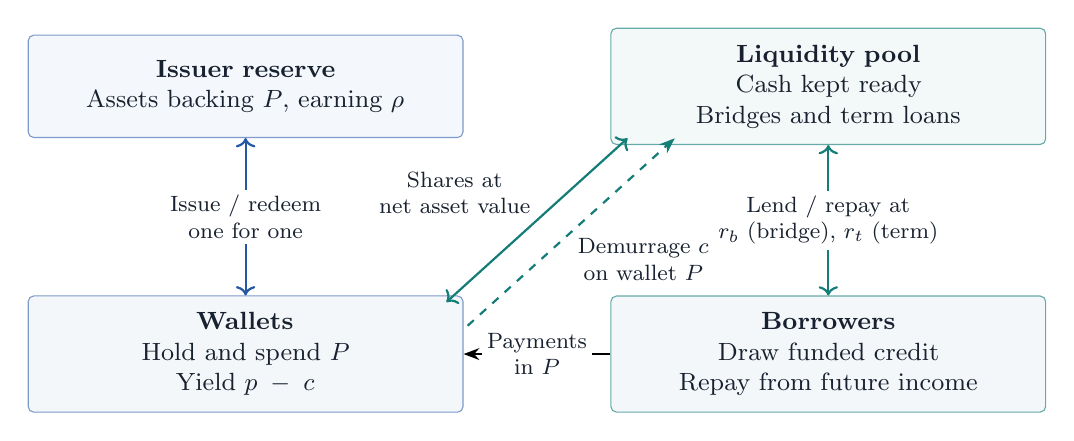
\begin{tikzpicture}[mapbox/.append style={minimum height=13mm}]
\node[mapbox,draw=blue!60,fill=blue!5,text width=5.1cm] (reserve) at (-3.7,3.4)
 {\textbf{Issuer reserve}\\Assets backing \(P\), earning \(\rho\)};
\node[mapbox,draw=teal!65,fill=teal!5,text width=5.1cm] (pool) at (3.7,3.4)
 {\textbf{Liquidity pool}\\Cash kept ready\\Bridges and term loans};
\node[mapbox,draw=blue!60,text width=5.1cm] (user) at (-3.7,0)
 {\textbf{Wallets}\\Hold and spend \(P\)\\Yield \(p-c\)};
\node[mapbox,draw=teal!65,text width=5.1cm] (borrower) at (3.7,0)
 {\textbf{Borrowers}\\Draw funded credit\\Repay from future income};
\draw[maparrow,blue,<->] (reserve)--node[maplabel]{Issue / redeem\\one for one}(user);
\draw[maparrow,teal,<->] (pool)--node[maplabel]{Lend / repay at\\\(r_b\) (bridge), \(r_t\) (term)}(borrower);
\draw[maparrow] (borrower.west)--node[maplabel]{Payments\\in \(P\)}(user.east);
\draw[maparrow,teal,<->] (-1.15,0.66)--node[maplabel,pos=.5,above left]{Shares at\\net asset value}(1.15,2.74);
\draw[maparrow,teal,dashed] (-0.88,0.36)--node[maplabel,pos=.5,below right]{Demurrage \(c\)\\on wallet \(P\)}(1.75,2.74);
\end{tikzpicture}
\caption{The reserve backs the payment money; its users own the pool. A
wallet balance earns \(p\), the reserve return less the issuer's custody
cost, and pays the holding charge \(c\), the demurrage, out of it to the
pool, so it yields \(p-c\). Pool shares earn the pool's own return and pay no
charge. The pool lends only money it holds. Wallets, owners and borrowers are
the same households in different roles.}
\label{fig:mechanism}
\end{figure}

\paragraph{The payment money.}
\(P\) is issued one for one against reserve assets and redeemable. The
reserve earns the outside rate \(\rho\). Issuance is contestable, so the
issuer keeps only its custody cost, and an idle unit of \(P\) earns
\(p=\rho-c_I\) before the holding charge, where \(c_I\) is that cost.
Payments in \(P\) settle on stablecoin rails and bear only the network cost
of a transfer, with no card-style fee. Section~\ref{sec:model} gives the cost
of a payment and a conversion in each arrangement; the comparison with the
decentralised arrangement does not rest on either.

\paragraph{The pool.}
A participant can move spare \(P\) into the pool and receives shares at net
asset value. The pool holds cash and loans. It makes two kinds of loan to
participants, both against future income and without collateral: a bridge,
drawn when a payment falls due before a receipt and repaid on the borrower's
next pay days, and a term loan repaid in instalments. The pool lends only
money it holds, so every loan is funded credit and no money is created.
Shares bear the pool's loan losses. An owner leaves by filing a redemption,
paid after a notice period.

\paragraph{What lets the pool lend without collateral.}
A protocol asks for collateral because it knows nothing of its borrower but
the assets locked with it. The pool is given three things a protocol lacks.
It sees the receipts a borrower expects over the next two months and lends a
bridge only up to what they repay. It collects a bridge that has fallen due
from all the borrower's money. And a debt stays owed when its borrower leaves
the network. The model adds that nobody who can pay chooses not to, and
sets no cost on establishing who a borrower is. These rules, not the
holding charge, separate the arrangement from decentralised finance
on the payments that fail; the demurrage decides what the credit costs and how
much of it is kept ready. They are stated as assumptions
(Section~\ref{sec:model}). What tests them is the loss on the pool's loans,
which its owners bear and its coupon prices (Section~\ref{sec:loss}), and a
bound under which the pool loses at the published charge-off rate of each
class of loan (Section~\ref{sec:measurement}).

\paragraph{The holding charge, or demurrage.}
Wallet balances of \(P\) pay a holding charge at rate \(c\): a demurrage, a
charge on money for the time it is held. Pool shares do
not. The rate is fixed and published at the start of each month from
quantities observed in the two months before, and the proceeds go to
the pool. A wallet balance therefore yields \(p-c\).

\paragraph{The people.}
There is no outside liquidity provider and no subsidy. The households that
hold \(P\), those that own the pool and those that borrow
from it are the same population, and each decides separately whether to
accept and pay in \(P\), to invest, to borrow and to
leave.

\paragraph{The comparisons.}
CPM is compared with four other arrangements on the same people
(Table~\ref{tab:arms}). The first two are the alternatives a household has
today. The third isolates the demurrage and the standby it pays for:
the same money and the
same pool with \(c=0\). The fourth states the contract in purchasing-power
terms.

\begin{table}[htbp]\centering\small
\begin{tabularx}{\linewidth}{@{}lLLl@{}}
\toprule
Arrangement & Money people hold & When a payer is short & Code \\
\midrule
Banks and cards & bank money & card within its limits, cash advance, earned-wage access, else the payment fails & \texttt{S0} \\
Best-case DeFi & bank money, or a yield-bearing stablecoin in the network & as banks and cards: its loan needs collateral
worth more than the loan and covers no shortfall & \texttt{M0} \\
Pool without the charge & bank money, or \(P\) in the network & the pool at the full coupon, then as banks and cards & \texttt{U} \\
CPM & bank money, or \(P\) less the holding charge & the pool at the coupon less what the charge covers, then as banks and cards & \texttt{M1} \\
Indexed CPM & as CPM, with \(P\) indexed to consumer prices & as CPM, the contract in real terms & \texttt{M2} \\
\bottomrule
\end{tabularx}
\caption{The five arrangements and their names in the code. The decentralised
arrangement is given every advantage it has in payments and yield, so that
CPM is measured against it at its best.}
\label{tab:arms}
\end{table}

% ====================================================================================================================
\section{The contract}
\label{sec:contract}
The contract sets five things each month: each loan product's coupon, the
holding charge, the price a bridge borrower pays, the pool's capital target,
and the return quoted to an entrant. This section states each as
the simulation computes it and gives the condition it is derived from.
Table~\ref{tab:notation} collects the notation.

\begin{table}[htbp]\centering\small
\begin{tabularx}{\linewidth}{@{}lL@{}}
\toprule
Symbol & Meaning \\
\midrule
\(\rho\) & reserve rate, equal to the outside rate \(r_{\mathrm{out}}\) \\
\(a\) & owners' alternative: what pool capital could earn elsewhere, \(\rho\) plus a declared spread \\
\(p\) & what idle \(P\) earns before the charge, \(\rho-c_I\) \\
\(o\) & the pool's operating cost per unit lent \\
\(\phi\) & the pool's fixed cost, per person per year; \(f\) is the same cost as a rate on lending \\
\(\ell_k\) & learned loss rate of product \(k\) (\(b\) bridge, \(t\) term) \\
\(r_k\) & coupon of product \(k\); \(r_g\equiv r_b^{\,\mathrm{gross}}\) is the bridge coupon before the charge \\
\(r_b\) & price a bridge borrower pays \\
\(c,\ \kappa\) & holding charge on wallet \(P\), the demurrage rate; coverage, the share of the capital cost the charge pays \\
\(\theta\) & demurrage's share of what finances bridging \\
\(B,\ T,\ L\) & bridge book, term book and their sum (principal-time) \\
\(S\) & standby: pool cash kept ready for bridging (cash-time) \\
\(W\) & wallet \(P\) held by participants (balance-time) \\
\(K\) & capital cost of the liquidity kept ready \\
\(N,\ N^{*}\) & pool capital at net asset value, and its target \\
\(q(N)\) & the return quoted to pool capital at level \(N\) \\
\(A,\ a_{0}\) & share of people participating, and that share at launch \\
\bottomrule
\end{tabularx}
\caption{Notation. Rates are stated a year and applied a month. A hat, as in
\(\cyc B\), is a sum over the cycle, the last two completed months.}
\label{tab:notation}
\end{table}

\subsection{Timing}
Terms are set at the start of a month from completed observations only. The
observation window is the cycle: the two months just closed. At launch, when
no month of pool activity exists, the window is a launch plan built from the
bridging need the initial participants showed the month before. The plan
observes no cost of liquidity, so the charge is zero in the launch month and
its bridges pay the full coupon. No term is a residual of the
month it applies to.

\subsection{The coupon}
Each pool loan of product \(k\) accrues a coupon
\begin{equation}
r_g \;=\; a+o+f+\ell_b ,\qquad r_t \;=\; a+o+f+\ell_t ,
\label{eq:coupon}
\end{equation}
floored at zero. The four parts are the four costs of a loan. Capital must
earn the owners' alternative \(a\). Lending has an operating cost \(o\) per
unit. The pool's fixed cost is spread over the lending that bore it,
\begin{equation}
f \;=\; \frac{\cyc\Phi}{\cyc L},
\label{eq:fixed}
\end{equation}
where \(\cyc\Phi\) is the cycle's fixed cost and \(\cyc L\) the
principal-time the pool's loans carried in it. Each product carries its
own learned loss rate \(\ell_k\) (Section~\ref{sec:loss}). Equation
\eqref{eq:coupon} is a zero-profit condition: coupons accrued at \(r_k\) on the
cycle's lending pay capital its alternative, the operating and fixed cost, and
the losses experienced so far, and nothing more. When the cycle carried no
loans, \(f\) is the fixed cost over the cycle's lending need.

\subsection{The liquidity kept ready and its cost}
The pool serves bridges on demand, so it must hold cash against the largest
demand it expects, not only the average. Let \(B_d\) be the bridging
principal carried on day \(d\) of the cycle and \(C_d\) the pool cash new
loans may take that day: pool cash less what is set aside for exits
falling due. The peak bridging need is
\begin{equation}
B^{\max} \;=\; \max_{d} B_d \;+\; \text{bridging refused in the cycle},
\label{eq:peak}
\end{equation}
and the standby is the cash held ready up to that peak beyond what was lent,
\begin{equation}
\cyc S \;=\; \sum_{d}\min\!\bigl(C_d,\ \max(B^{\max}-B_d,\,0)\bigr),
\label{eq:standby}
\end{equation}
in cash-time. Standby is measured, not reserved: it is the cash
available up to the peak, and no rule holds it back from term lending. Money
out in bridges must earn \(a\). Cash standing by earns
\(p\) as any idle \(P\) does, so it falls short of \(a\) by \(a-p\). The
capital cost of the liquidity kept ready over the cycle is therefore
\begin{equation}
K \;=\; a\,\cyc B \;+\;(a-p)\,\cyc S .
\label{eq:cost}
\end{equation}

\subsection{The demurrage rate and the bridge price}
The holding charge, the demurrage rate \(c\), is the rate at which the cycle's
wallet balances would have paid
that cost, capped so a wallet balance never earns less than nothing:
\begin{equation}
c \;=\; \min\!\Bigl(\frac{K}{\cyc W},\ p\Bigr),
\label{eq:charge}
\end{equation}
with \(c=0\) when the cycle shows no wallet balances and whenever the pool
takes no charge, because it has no shares or is winding down. Coverage is the
share of the cost the charge pays,
\begin{equation}
\kappa \;=\; \min\!\Bigl(1,\ \frac{c\,\cyc W}{K}\Bigr),
\label{eq:coverage}
\end{equation}
which is one whenever the cap in \eqref{eq:charge} does not bind. A bridge
drawn in the month is sealed at the coupon less the covered capital part,
\begin{equation}
r_b \;=\; r_g-\kappa\,a ,
\label{eq:bridgeprice}
\end{equation}
so at full coverage the borrower pays \(o+f+\ell_b\). Term loans pay the full
coupon \(r_t\). A wallet balance yields
\begin{equation}
y \;=\; p-c ,
\label{eq:yield}
\end{equation}
to which indexed CPM adds the change in the price index. In the pool without
the charge, \(c=\kappa=0\) and \(r_b=r_g\).

\subsection{The capital target and the quote}
The pool's capital target is the capital the cycle's lending needed, with
bridging counted at its peak:
\begin{equation}
N^{*} \;=\; T^{\mathrm{need}}+B^{\max},
\label{eq:target}
\end{equation}
where the term lending need \(T^{\mathrm{need}}\) is the term principal
carried, plus term lending refused, plus the month's growth in the term book
floored at zero, averaged over the cycle's months. In the pool without the
charge nothing pays for standby, and the target is the average lending need,
bridges and term loans alike, with no peak. The return quoted to
capital at level \(N\) is the alternative on capital up to the target and the
idle rate on the rest:
\begin{equation}
q(N) \;=\; \frac{a\,\min(N,N^{*})+p\,\max(N-N^{*},0)}{N},
\qquad q(N^{*})=a .
\label{eq:quote}
\end{equation}
Equation \eqref{eq:quote} is the free-entry condition with no fee margin. The
coupons \eqref{eq:coupon} and the charge \eqref{eq:charge} pay capital exactly
\(a\) on the liquidity kept ready, so \(N^{*}\) is the largest capital at
which an entrant is offered its alternative.

\subsection{Entry and exit}
\label{sec:entry}
The contract fixes how capital enters and leaves the pool. When a household
chooses to enter or leave is behaviour and belongs to the model of
Section~\ref{sec:model}; it is stated here because
Proposition~\ref{prop:capital} rests on it.
Dealing is monthly. Each month a household reviews its savings with a fixed
probability \(\upsilon\), the rate at which members and owners review
leaving. A
reviewing household offers the money-market part of its spare money to the
pool if the quote at the target, \(q(N^{*})\), is at least its own
alternative; an owner with an exit request standing offers nothing. Offers
are accepted in proportion up to the room, which is \(N^{*}-N\) when that is
positive plus any exits pool cash has left unpaid. Owners review their
holding at the same rate \(\upsilon\). A reviewing owner files to redeem all
of it with probability
\begin{equation}
\Pr(\text{file}) \;=\; \frac{1}{1+e^{\,(g+h)/s}},
\label{eq:exit}
\end{equation}
where \(g\) is the owner's realised return over the last twelve months less
its alternative, times its own capital, in dollars a month; \(h\) is its cost
of leaving, zero for an owner in the network and, for one who has left it,
the conversion fee on the holding spread over twelve months; and \(s\) is a
noise scale proportional to the owner's monthly spending. For an owner in the
network the probability at exact indifference is one half. A request stands
until it is paid or a later review no longer says leave. It is paid at
the first dealing at least two months after it was filed, from pool cash and
in proportion when cash is short; a dealing's new subscriptions buy the
part pool cash leaves unpaid before they take up room.

\subsection{Loss learning}
\label{sec:loss}
A pool loan ninety days past due is written down to zero, principal
and accrued interest; the debt stays owed and later payments, interest
included, are recoveries. The learned loss rate of product \(k\) is the
pool's whole experience,
\begin{equation}
\ell_k \;=\; \frac{\max\bigl(\text{write-offs}_k-\text{recoveries}_k,\ 0\bigr)}
{\text{principal-time of product }k\text{ carried up to three months before the last close}} ,
\label{eq:loss}
\end{equation}
the lag being the time a missed payment takes to become a loss.

% ====================================================================================================================
\section{What the contract implies}
\label{sec:implications}
This section derives the properties of the contract of
Section~\ref{sec:contract}. Each is a statement about equations
\eqref{eq:coupon} to \eqref{eq:loss} and holds in the simulation by
construction or as a prediction. Section~\ref{sec:results} sets the
predictions beside their simulated values, and Section~\ref{sec:robustness}
tests the fixed-cost threshold.

\subsection{The size of the demurrage}
\begin{proposition}[Demurrage is the alternative times bridging over balances]
\label{prop:size}
While the cap in \eqref{eq:charge} does not bind, coverage is one and
\begin{equation}
\frac{c}{a} \;=\; \frac{\cyc B}{\cyc W}+\Bigl(1-\frac{p}{a}\Bigr)\frac{\cyc S}{\cyc W}.
\label{eq:size}
\end{equation}
The cap binds if and only if \(K>p\,\cyc W\).
\end{proposition}
\begin{proof}
Divide \eqref{eq:cost} by \(a\,\cyc W\). If \(K\le p\,\cyc W\) then
\(c=K/\cyc W\) and \(c\,\cyc W/K=1\); otherwise \(c=p\) and
\(\kappa=p\,\cyc W/K<1\).
\end{proof}
The second term of \eqref{eq:size} is small, because \(a-p\) is only the
owners' spread plus the issuer's custody cost. The demurrage rate is therefore close
to \(a\,\cyc B/\cyc W\): it is small because people hold many times more
money in wallets than the pool has out in bridges. The cap would bind only if
bridging approached the size of wallet balances.

\subsection{Who pays and who receives}
\begin{proposition}[Incidence at full coverage]
\label{prop:incidence}
Let \(\kappa=1\) and let quantities over a cycle be \(\cyc B\), \(\cyc S\),
\(\cyc W\). Then, relative to the same pool with \(c=0\) at the same
quantities:
(a) holders pay \(K\) in total, in proportion to their balances;
(b) bridge borrowers pay \(a\,\cyc B\) less;
(c) owners receive \((a-p)\,\cyc S\) more, and so earn \(a\), after costs and
expected loss, on every unit kept ready, whether it is lent or standing by.
The three amounts sum to zero.
\end{proposition}
\begin{proof}
(a) By \eqref{eq:charge}, \(c\,\cyc W=K\). (b) By \eqref{eq:bridgeprice} the
bridge price falls by \(a\). (c) The pool's income on liquidity kept ready is
\((r_g-a)\cyc B\) from borrowers, \(K\) from the charge and \(p\,\cyc S\) on
its cash, which is \(r_g\,\cyc B+a\,\cyc S\) by \eqref{eq:cost}; without the
charge it is \(r_g\,\cyc B+p\,\cyc S\). Finally
\(-K+a\,\cyc B+(a-p)\cyc S=0\).
\end{proof}
\begin{corollary}[Neutrality at fixed quantities]
\label{cor:neutral}
With all quantities held fixed, total household wealth under CPM equals total
household wealth under the same pool without the charge.
\end{corollary}
The corollary fixes what the simulation can and cannot show. Demurrage moves
the capital cost of bridging from households that are short to all
holders, and makes standing by pay. It does not create wealth by itself.
Any aggregate difference between CPM and the pool without the charge must
come from quantities that change: the standby the target
\eqref{eq:target} now includes, the bridges then served, and the
payments that no longer fail.

\subsection{Demurrage's share of bridging finance}
Let \(\theta\) be the part of the cost of bridging that demurrage carries:
the capital cost covered, over that amount plus the coupons bridge borrowers
pay.
\begin{proposition}[The share]
\label{prop:theta}
Let every bridge carried in a month have been sealed at full coverage. Then
\(\theta=a/\bar r_g\), where \(\bar r_g\) is the gross coupon of those
bridges at the months they were sealed, weighted by their principal-time. In
particular \(\theta=a/r_g\) when the coupon is constant, and the ceiling of
\(\theta\), reached when the fixed-cost rate and the bridge loss rate vanish,
is \(a/(a+o)\).
\end{proposition}
\begin{proof}
A bridge sealed in month \(m\) with principal-time \(x\) has \(a\,x\) of its
coupon paid by the charge and pays \((r_{g,m}-a)\,x\) itself, by
\eqref{eq:bridgeprice}. Summing over the bridges carried,
\(\theta=a\sum x/\sum r_{g,m}x\). By \eqref{eq:coupon}, \(r_{g,m}\ge a+o\)
with equality when \(f=\ell_b=0\).
\end{proof}
The share rises with the outside rate, since \(a\) does, and falls when
losses or a thin book raise the coupon. A bridge runs to the borrower's next
pay day, often across a month end, so the bridges carried in a month were
sealed in more than one; the simple form \(a/r_g\) is exact only when the
coupon has not moved between those months.

\subsection{What holds pool capital in place}
\begin{proposition}[Capital at the target]
\label{prop:capital}
Suppose that at each dealing the money offered exceeds the room and that
entrants act on the quote. Then after every dealing
\begin{equation}
N \;=\; \max\bigl(N^{*},\ N^{-}\bigr),
\label{eq:capital}
\end{equation}
where \(N^{-}\) is capital after the exits paid at that dealing. No realised
return appears in this law of motion.
\end{proposition}
\begin{proof}
By \eqref{eq:quote}, \(q(N^{*})=a\) in every month, so the entry test of
Section~\ref{sec:entry} passes for every household whose alternative is at
most \(a\). Offers are accepted up to \(N^{*}-N^{-}\) when that is positive
and not at all otherwise.
\end{proof}
The proposition is conditional, and the condition matters. The
quoted schedule \eqref{eq:quote} is flat at \(a\) for all capital up to the
target, so the contract contains no return gradient that pulls capital back
when it falls short. This is the knife-edge of a pool that pays capital
exactly its alternative: every capital level up to the target is an
equilibrium, and the entry rule selects the level. Capital persists at
its target if entrants act on the published quote and the quote is right on
average. If entrants act on the pool's realised record instead, entry closes
whenever that record sits below \(a\), which under a zero margin is about
half the time. We call the first the quote rule and the second the record
rule, and Section~\ref{sec:results} reports the simulation under both.

\begin{proposition}[The quote is right on average under a stationary loss rate]
\label{prop:fair}
Let \(R\) be the realised return on pool capital \(N\) over a period in which
the pool carries loans \(L=B+T\) and cash \(C\), bears fixed cost \(\Phi\) and
net losses \(\Lambda\), and collects charges \(cW\). Then
\begin{equation}
(R-a)\,N \;=\; \underbrace{\textstyle\sum_k \ell_k L_k-\Lambda}_{\text{loss pricing}}
\;+\;\underbrace{fL-\Phi}_{\text{fixed-cost timing}}
\;-\;\underbrace{(a-p)\,(C-S^{\mathrm{paid}})}_{\text{idle drag}},
\qquad S^{\mathrm{paid}}=\frac{cW-\kappa\,a\,B}{a-p},
\label{eq:identity}
\end{equation}
where \(S^{\mathrm{paid}}\) is the standby the charge paid for. If the loss
rate is stationary, the learned rate \eqref{eq:loss} converges to it and the
loss-pricing term has mean zero.
\end{proposition}
\begin{proof}
The pool's assets are its loans, with the coupons accrued on them, and its cash,
so \(N=L+C\). Its income is the
coupons borrowers pay, \(\sum_k r_kL_k-\kappa aB\), the charge \(cW\), and
\(p\,C\) on its cash; its costs are \(oL\), \(\Phi\) and \(\Lambda\).
Substituting \eqref{eq:coupon} and subtracting \(aN=aL+aC\) leaves
\((fL-\Phi)+(\sum_k\ell_kL_k-\Lambda)+cW-\kappa aB-(a-p)C\).
\end{proof}
The identity is the pool's income statement rearranged, and says where an
owner's shortfall can come from. The fixed-cost term is a timing difference:
\(f\) is set on the last cycle's lending and earned on this period's. The
idle drag is the cost of cash beyond the standby. Both are small. The loss
term is a tail: a loss larger than the pool's experience falls on those
who own the pool on the day of the write-down, and it shrinks as the number
of borrowers grows.

\subsection{The fixed cost}
A pool that prices loans as the residual of its costs over its lending,
\(r=z+\Phi/L(r)\) with \(z\) the variable cost of a loan, can spiral: fewer borrowers raise the price, and a higher
price loses borrowers. Under this contract the same fixed cost appears
in \eqref{eq:fixed}, so the question is whether the spiral survives.
\begin{proposition}[A threshold, not a spiral]
\label{prop:threshold}
Let a borrower take pool credit only if its coupon is no dearer than the
borrower's outside rate \(r_{\mathrm{ext}}\), and let \(L_0\) be the lending
then demanded. A coupon satisfying \eqref{eq:coupon} and \eqref{eq:fixed}
with positive lending, \(L_0>0\), exists if and only if
\begin{equation}
L_0\,\bigl(r_{\mathrm{ext}}-a-o-\ell\bigr) \;\ge\; \Phi .
\label{eq:threshold}
\end{equation}
\end{proposition}
\begin{proof}
Demand is a step: \(L=L_0\) if \(r\le r_{\mathrm{ext}}\) and zero otherwise.
With \(L=L_0\) the coupon is \(a+o+\ell+\Phi/L_0\), which is at most
\(r_{\mathrm{ext}}\) exactly when \eqref{eq:threshold} holds. When the margin
\(r_{\mathrm{ext}}-a-o-\ell\) is zero or negative no lending satisfies it.
\end{proof}
Below the threshold the pool does not lend, and \eqref{eq:fixed} prices the
fixed cost on the lending need, which grows with participation. The pool
then crosses the threshold later. The fixed cost delays formation at low
adoption; it does not unwind a pool that has formed.

\subsection{Participation}
In the model a household outside the network joins with a probability that
rises with the share of its contacts already in it, and a participant leaves
on its own experience (Section~\ref{sec:model}). With contact equal to the
participating share \(A\), base joining rate \(j_0\), contact rate \(j_1\)
(the model's \(\xi_0\) and \(\xi_1\)) and
realised leaving rate \(\lambda\), participation follows
\begin{equation}
A_{t+1} \;=\; A_t+(j_0+j_1A_t)(1-A_t)-\lambda A_t .
\label{eq:diffusion}
\end{equation}
\begin{proposition}[Launch adoption is a date on one curve]
\label{prop:diffusion}
Let \(j_0,\lambda>0\) and let the map \eqref{eq:diffusion} be increasing in
\(A_t\), as it is for monthly rates of the size used here. Then
\((j_0+j_1A)(1-A)=\lambda A\) has exactly one root \(A^{*}\) in \((0,1)\),
every path converges to it, and the path from a launch share
\(a_0'<A^{*}\) lies between two consecutive monthly shifts of the path from
any lower launch share \(a_0\).
\end{proposition}
\begin{proof}
The left side less the right is a downward parabola in \(A\) that is positive
at zero and negative at one, so it has one root in \((0,1)\), and
\(A_{t+1}-A_t\) has its sign on either side. An increasing map preserves
order and keeps a path that starts below \(A^{*}\) below it. The path from
\(a_0\) therefore rises to \(A^{*}\) without passing it and brackets every
share between \(a_0\) and \(A^{*}\): there is a \(\tau\) with
\(A_\tau\le a_0'\le A_{\tau+1}\), and the path from \(a_0'\) then stays
between that path shifted by \(\tau\) and by \(\tau+1\) months. Two launch
shares on opposite sides of \(A^{*}\) are not bracketed in this way; every
launch level of the grid lies below it.
\end{proof}
The mechanism therefore acts on participation only through the leaving rate
\(\lambda\). A launch share is a starting date, and a comparison across launch
shares within a fixed horizon compares earlier and later phases of the same
growth.

% ====================================================================================================================
\section{The model}\label{sec:model}

This section describes the agent-based model that carries the contract of Section~\ref{sec:contract} into a
population of households, in the order of the ODD protocol \cite{grimm}. Every statement below is read from
the simulation code. All parameter values and sources are in Appendix~\ref{app:parameters}.
Table~\ref{tab:onepage} first gives the whole model on one page: its objective, its assumptions,
the agents, their state, the control parameters, the dynamics, what each agent optimises, the remaining
equations and what emerges.

\begin{table}[p]
\centering\footnotesize
\caption{The model on one page.}\label{tab:onepage}
\begin{tabularx}{\textwidth}{@{}p{0.17\textwidth}X@{}}
\toprule
Objective & To find whether a payment money whose holders pay a small holding charge, a demurrage, can fund one pooled liquidity
  buffer that lends to its own users without collateral; whether that pool forms and persists with no outside
  support; and who gains or loses against banks and cards and against best-case DeFi. \\
\addlinespace
Assumptions & (i) Total spending is fixed; there is no production and no growth.
  (ii) The pool sees a borrower's expected receipts, lends a bridge only up to what they repay, collects a due
  bridge from all the borrower's money, and a debt survives leaving the network; nobody who can pay chooses not to.
  (iii) A DeFi loan needs collateral worth more than the loan, so it covers no shortfall.
  (iv) People act on their own last month and last year and form no forecast.
  (v) Savers enter on the pool's published quote, the quote rule; a second map has them enter on its realised
  return, the record rule.
  (vi) The reserve rate is constant within a run, and outside deposit and loan rates follow it.
  (vii) The five arrangements face the same people and the same random draws. \\
\addlinespace
Agents and network & People, each one consumer unit, who pay and are paid, hold money, borrow and may own pool
  shares. Three collective entities: the pool, the issuer of P and the outside lenders. People are joined by a
  payment network: each pays one wage to one other person, fixed for the run, and makes 32 service purchases a
  month from sellers drawn afresh each month, uniformly over everyone else, so one person's spending is other
  people's income. Section~\ref{sec:robustness} replaces the uniform draw by a ring and by hub sellers. \\
\addlinespace
State variables & Of a person: bank money $E$, P once in the network, outside savings, pool shares, invoices
  receivable and payable, card balance and loans, and whether it is in the network. Its fixed traits are its
  spending weight, billing and pay cycles, the one wage it pays, its card, score and line. In aggregate:
  participation $A$; pool capital $N$ and its target $N^{*}$; the pool's term book $T$, bridge book $B$ and cash $C$;
  wallet balances $\cyc W$, bridging $\cyc B$ and standby cash $\cyc S$ over a cycle; the learned loss rates
  $\ell_{k}$. \\
\addlinespace
Control parameters & The reserve rate $\rho$, launch participation $a_{0}$ and the extra layoff rate of the
  distress year. The first and third are the environment and the second is the condition a launch starts from. The
  design is the contract, the same in every cell and compared across five arrangements. \\
\addlinespace
Dynamics & \emph{Each day} the payments due settle together, as the fixed point $\sigma = F(\sigma)$ of the shares each
  payer completes (Proposition~\ref{prop:settlement}).
  \emph{Each month} every person re-chooses a cash buffer; a person outside joins with chance
  $\xi_{0} + \xi_{1}s_{i}$, where $s_{i}$ is the share of its trading partners in the network; members, owners
  and savers review leaving, exit~\eqref{eq:exit} and entry with chance $\upsilon$; and the pool sets its coupon,
  charge, target and quote from the cycle just closed.
  \emph{In aggregate} participation follows $A_{t+1} = A_{t} + (j_{0} + j_{1}A_{t})(1 - A_{t}) - \lambda A_{t}$
  \eqref{eq:diffusion} and capital returns to $N = \max(N^{*}, N^{-})$ at each dealing when offers exceed the room
  \eqref{eq:capital}. Section~\ref{sec:laws} writes the laws of motion of the aggregate state, \eqref{eq:law-A} to
  \eqref{eq:law-W}, month by month and in continuous time. \\
\addlinespace
Objective functions & No agent optimises over the world.
  \emph{A person} keeps the cash buffer, from a fixed grid, that would have cost it least over its own last month:
  return given up, credit cost, fees and failure fees.
  \emph{A member} leaves with a logistic probability in its own experienced gain over the last year;
  \emph{an owner} files to redeem by~\eqref{eq:exit} on its realised return against its alternative;
  \emph{a saver} offers its money when the quote $q(N^{*})$ is at least its alternative.
  \emph{The pool} maximises nothing: its prices solve zero-profit and free-entry conditions, the coupon
  $r_{k} = a + o + f + \ell_{k}$ \eqref{eq:coupon}, the demurrage rate $c = \min(K/\cyc W,\, p)$ \eqref{eq:charge} and the
  quote $q(N^{*}) = a$ \eqref{eq:quote}. \\
\addlinespace
Further equations & The cost of the liquidity kept ready, $K = a\,\cyc B + (a - p)\,\cyc S$ \eqref{eq:cost}; the
  bridge price $r_{b} = r_{g} - \kappa a$ \eqref{eq:bridgeprice}; the wallet yield $y = p - c$ \eqref{eq:yield};
  the capital target $N^{*} = T^{\mathrm{need}} + B^{\max}$ \eqref{eq:target}. From them, the size of the demurrage,
  $c/a = \cyc B/\cyc W + (1 - p/a)\,\cyc S/\cyc W$ (Proposition~\ref{prop:size}), and the lending a pool needs to
  carry its fixed cost, $L_{0} \ge \Phi/(r_{\mathrm{ext}} - a - o - \ell)$ (Proposition~\ref{prop:threshold}). \\
\addlinespace
Emergence & Nothing below is set; each arises from the decisions above and the contract applied to what they
  produce. Participation $A$ and its path; pool capital and whether it holds its target, $N/N^{*}$; the coupons,
  the demurrage rate $c$, the bridge price $r_{b}$ and demurrage's share $\theta$ of bridging finance; the share
  of payments that fail; each person's gain against the bank arrangement and against best-case DeFi; and, under
  distress, a run on the pool when owners file to leave after a write-off. These are the order parameters, each
  defined in Section~\ref{sec:measurement}. \\
\bottomrule
\end{tabularx}
\end{table}

\subsection{Purpose and patterns}

The model asks whether a payment money whose holders pay a small holding charge can fund one pooled liquidity
buffer that lends to its own users, whether that pool forms and persists without outside support, and who gains or
loses against today's arrangements. It plays the same simulated people, with the same random events, through five
arrangements (Table~\ref{tab:arms}), so any difference between two arrangements for one person comes from the
arrangement alone. Best-case DeFi gives stablecoin payments and a yield on balances, and no credit to a payer who
is short, since its loan needs collateral worth more than the loan. The pool without
the charge is CPM's contract with the charge set to zero. Nothing then pays for cash standing by, so
its capital target is the average lending need with no peak \eqref{eq:target}. CPM against it therefore shows
what demurrage and the liquidity it pays for add together.

The model compares designs and forecasts nothing. No output predicts a quantity in the United States
economy. The patterns below check the bank arrangement (banks and cards) against data; the new arrangements do not exist to be
checked. The theory of Section~\ref{sec:implications} is the minimal model, written in a few aggregate
quantities. The simulation adds what that theory averages over: people who differ and a network of payments. It also adds
the detail of cards, fees and credit lines that prices today's alternative, since a gain measured against a cheaper
alternative than people have would not be a gain.

Total spending is fixed and there is no production, so the model compares how the same spending is paid and
financed. It is checked against a few patterns and is not fitted to them: the stock of jobs
without a wage under normal job loss (about 1.9\% of jobs, against about 2.0\% of US payroll jobs in 2026), the
tier mix of card holders and their lines against the CFPB's card market report, the scale of the distress year
against the fall in US wages in 2009, and holders' use of cash advances, which runs above the US level and is
allowed for by the cash-advance bound of Section~\ref{sec:measurement}.

\subsection{Entities, state variables and scales}

The agents are people, each standing for one US consumer unit. A person holds bank money $E$, and once in the
network P (USDC in best-case DeFi); one-month outside savings; pool shares valued at net asset value; invoices
receivable and payable; card balances; and loans by lender and kind (pool and outside bridges, instalment loans,
revolving card balances, cash advances, charged-off card balances, rounding overdrafts at a fixed outside rate and
interest-free failure-fee debt). Fixed traits drawn at the start are spending weight, billing cycle and phase, the
one other person it pays a wage to, the pay period and phase of that job, card holding, credit score, card line and
starting balance, whether its income is business receipts, and whether it holds earned-wage access. Net financial
wealth is money, savings, shares and receivables less payables, card balances and every loan; illiquid wealth and a
card's starting balance are outside it.

Three collective entities hold state. The pool holds its cash, its loan book (bridge book $B$, term book $T$), its
standby cash $S$ and its capital $N$, owned by households alone, against its target $N^{*}$. The issuer holds the
reserves behind all P, keeps its custody cost and owns no shares. Outside lenders, card networks, the conversion
provider, the pool's operating provider, validators and the issuer sit outside the household economy and hold no
state beyond the flows recorded with them.

Money is measured in months of mean consumer-unit spending, one unit being \$6,440. Time runs in days of a 30-day
month. A run is a burn-in of six months under the bank arrangement, shared exactly by every arrangement, followed by
60 months after launch. The pool forms by free entry from the first dealing with a lending need. The confirmation
maps and the final development map use 4,000 people; development checks used 1,000.

Figure~\ref{fig:wagenet} draws the wage links of one population. Each person pays one wage to one other person, so
the links form long chains and branches, and a wage that fails has one path onward.

\begin{figure}[htbp]\centering
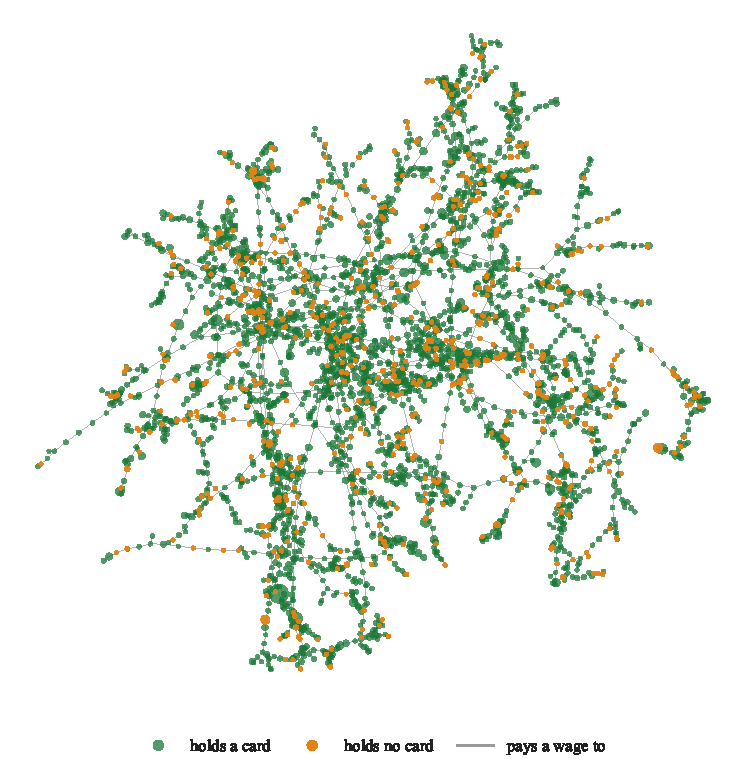
\includegraphics[width=0.8\linewidth]{figures/fig_wage_network.pdf}
\caption{The wage network of one population draw: \NumPeople{} people at the first confirmation seed. Each person
pays one wage to one other person. A node's area follows the person's spending. Purchases, which link each person
to many sellers a month, are not drawn.}
\label{fig:wagenet}
\end{figure}

\subsection{Process overview and scheduling}

Each month runs in this order.
\begin{enumerate}[leftmargin=*,itemsep=1pt]
\item At the launch month only, people are drawn into the network with probability $a_{0}$ and convert their bank
money into P at one conversion fee.
\item Jobs are laid off at the normal rate, plus the distress control's extra rate in the distress year; the month's
service purchases, wage accruals and instalment-credit requests are created.
\item The pool publishes its terms from the last two completed months: the bridge and term coupons, the capital
target $N^{*}$ and the quote at it, the holding charge $c$, its coverage $\kappa$ and the yield on P.
\item Dealing: outside savings mature into cash; owners who review may file to exit and due exits are paid; what is
already due is collected, then overdue wages, then every debt, all from all money; each person chooses a cash buffer
by replaying its own last month; spare money is split into pool offers and outside savings.
\item Thirty days of settlement. Each day: earned-wage accrual; arrears flags; instalments falling due, collected
from all cash and same-day savings; instalment purchases settling that day; the day's bills and wages, with
bridging, cash advances, earned-wage advances and failures; on day 20 the card statement, its minimum payment and
any late fee; the day's own cash flow is recorded for next month's replay; what is due is collected from all money
(missed instalments, then outside bridges dearest first, then pool bridges); overdue wages and then other debts are
repaid from money above the buffer; interest and the pool's operating cost accrue; pool loans 90 days past due are
written down; cards 180 days past due are charged off.
\item The month's card purchases are billed on the statement due on day 20 of the next month.
\item Close: savings earn their rate; the reserve return on P pays wallet holders their yield net of the charge and
pays the charge and the pool cash's return to the pool; the pool pays its fixed cost, its value per share and the
owners' realised return are set, and the month is entered in the record the next terms read; experience of using
the network is computed; people leave and join; card rewards are paid; durables depreciate; consumer prices deflate
every nominal stock; next month's spending is set; records are written.
\end{enumerate}

\subsection{Time and updating}\label{sec:updating}

The clock is the day, the same for every population size. No rule visits people one after another and none draws a
visiting order: every rule applies to all people in one step, and chance enters as an independent draw for each
person. Results can depend on the update scheme, a known hazard of agent-based models
\cite{huberman,axtell}, so the scheme is stated here and tested in Section~\ref{sec:robustness}. Three kinds of event
update in three ways.

\emph{Calendar events} fall on dates that contracts set: wages on each job's pay dates, bills on each seller's
billing date, instalments on the borrower's billing date, the card statement on day 20, the pool's terms at the
start of a month. Cycles of 1, 7, 15, 30 and 60 days on random phases spread these dates over the month, so people
are not in step. A monthly calendar with a fixed sequence of markets is the common choice in such models
\cite{baptista,poledna}. Within a day the pool's cash goes first to instalment purchases, then to bridges and, on
day 20, to card statements, pro rata to requests within each.

\emph{Decisions} are reviewed monthly. Leaving, owners' exit and savers' entry are each reviewed by a random part
of the people concerned, a person with chance $\upsilon = 1 - e^{-0.166}$ a month. That is the exact monthly chance
of a review clock that rings at rate 0.166 \cite{gillespie}, so these are random asynchronous updates at
monthly resolution. Joining is a chance of at most 3.4\% a month for each person outside. Leaving and joining
read the month's participation before either is applied. One decision is taken by everyone in the same dealing:
the cash buffer, chosen by the rule given under adaptation in the design concepts below.
Section~\ref{sec:robustness} repeats the runs with only a random part of the population
re-choosing its buffer each month. The diffusion equation \eqref{eq:diffusion} and the contract's identities are
written month by month, on the model's own clock.

\emph{Settlement} of a day's payments is simultaneous, because what a payer can pay depends on what it is paid
that day. Let $\sigma_{i}\in[0,1]$ be the share of its payments due on a day that payer $i$ completes, and $F$ the day's
map from every payer's share to the shares their receipts then allow. Cover is taken in the fixed order of the
submodel below and the pool's queue is held fixed. The day's outcome is a fixed point $\sigma = F(\sigma)$, found by repeating
$F$ from $\sigma = 1$ until no share moves by more than $10^{-14}$.

\begin{proposition}[Settlement]\label{prop:settlement}
(i) On a day on which the pool's cash covers every request it admits, and on every day in the arrangements without
a pool, $F$ is monotone, and the iteration from $\sigma = 1$ stops at the greatest fixed point of $F$.
(ii) With the day's credit taken as given, the fixed point is unique if and only if no set of payers completes a
positive share while its members have no means of their own that day and are paid that day only by one another.
Such a set pays only its own members.
(iii) With the day's credit taken as given, settlement one payer at a time in any order, each paying what it can
across its payments as money arrives until nothing more can be paid, ends at the least fixed point, and so at the
same outcome as the simultaneous solution whenever (ii) gives uniqueness.
\end{proposition}

\begin{proof}[Sketch]
(i) Receipts do not fall when any payer's share rises, and a payer's shortfall does not rise with its receipts. The
part of a shortfall left after each source of cover does not fall as the shortfall rises: savings, the cash advance
and earned-wage access are capped amounts, and the pool lends the largest draw that its receipts test admits for
that draw and every smaller one, which leaves an unlent part that cannot fall (a test checks this over the test's
parameter ranges). So $F$ is monotone. From $F(1)\le 1$ the iterates fall, and they stay above every fixed point
$g$, since $g = F^{k}(g) \le F^{k}(1)$; the point at which they stop is therefore the greatest.
(ii) With means $m_{i}$, dues $d_{i}$ and receipts $R_{i}(\sigma)$, the map is $F_{i}(\sigma) = \min\{1, (m_{i} +
R_{i}(\sigma))/d_{i}\}$. Let $\sigma$ be the greatest fixed point, $\sigma'$ another, and $D$ the payers with
$\sigma_{i} > \sigma'_{i}$. Each member of $D$ pays all it has under $\sigma'$, so
$d_{i}(\sigma_{i} - \sigma'_{i}) \le R_{i}(\sigma) - R_{i}(\sigma')$, and the right side is
what members of $D$ pay $i$ more under $\sigma$. Summing over $D$, the extra paid by $D$ is at most the extra $D$ pays
to its own members, which is at most the extra paid by $D$. Equality throughout means $D$ pays only its own
members; summing what its members pay under $\sigma'$ then gives that their means and their receipts from outside $D$
are zero. Conversely, the shares of such a set can be scaled down together and remain a fixed point.
(iii) By induction no payer's cumulative payment exceeds what it pays at the least fixed point, and where the
process ends no payer can pay more, which is a fixed point.
\end{proof}

Part (i) is the fictitious default algorithm of \cite{eisenbergnoe}: the payers who fail in its first round would
fail even if paid in full, and the rest fail because others did \cite{elsinger}. Part (ii) names the one case in
which the simultaneous solution does more than a sequence of payments could: a closed loop of payers without
money, who all pay in the model's solution and none of whom could pay first. Payment systems call that state
gridlock and resolve it by settling the loop at once \cite{bech}. The model's choice is the same in every
arrangement and leans toward completion. Every run records, each day, the payments that rest on it; they are
at most \NettingShareMost{} of completed value in any run (Section~\ref{sec:robustness}). When the pool's cash is short,
requests are served pro rata and $F$ need not be monotone, since a borrower with more receipts can ask for more and
cut every other borrower's share. The code detects two states that repeat and defers, for the day, the request
admitted in one and refused in the other. Within a day money received can be paid on, and the day has no
earlier and later; this too is the same in every arrangement.

\subsection{Design concepts}

\emph{Emergence.} Participation, pool capital, the coupons, the holding charge and failed payments are not set; they
arise from individual buffer, joining, leaving, entry and exit decisions and from the pool's rules applied to what
those decisions produce. The demurrage rate is computed each month from the bridging and standby cash the
pool kept ready over the last two months and from the wallet P balance $W$ held over them. Participation $A$ is
the share of people in the network during each month, before its month-end joining and leaving.

\emph{Adaptation.} People follow their own experience and do not optimise over the world. A person keeps the cash
buffer, from a fixed grid of multiples of its own spending, that would have cost least had it faced its own last
month again, counting the return given up, credit cost, cash-advance and earned-wage fees and failure fees. For a
member with no shortfall in that month the choice also reads the share of requests the pool served. A
member reviews its membership with the monthly chance $\upsilon$ of Section~\ref{sec:updating} and leaves with a logistic
probability that its average monthly experience over the last year falls short of one conversion of its average P
balance spread over that year. Owners review on the same rule with their own realised return against their
alternative. Savers review entry with the same probability and offer their money-market part when the pool's
published quote is at least their alternative.

\emph{Interaction.} People interact through the payment network: one person's spending is other people's income,
so a failed or late payment is missing income for its payee on that day. They also interact through the pool, whose
cash is rationed pro rata among borrowers on a day, and through joining, which rises with the share of a person's
own counterparties in the month who already use the network.

\emph{Stochasticity and common random numbers.} Each random stream has its own seed: the population's traits, the
job-loss stock at the start, each month's layoffs, purchases, shocks and credit requests, joining and leaving draws,
owners' draws and savers' entry draws. Every stream is drawn in every arrangement and month,
used or not, so all five arrangements see the same numbers. For one seed every arrangement therefore draws the same
population, the same obligations on the same dates and the same job-loss spells. What differs is the arrangement's
rules from launch on and, through them, what people choose: their buffers, participation and borrowing.
Initial wealth is not drawn: it is the mean of each equal quantile band of the Pareto law, so every seed has the same
wealth vector and seeds vary only the economy's events. Within a month one uniform draw per job decides its layoff at
every distress level, so a higher level's layoffs contain a lower level's and every level shares the months before
the distress year.

\emph{Observation.} Each run records monthly aggregates and, by person and month, net wealth, participation, pool
ownership and borrowing, completed and lost purchases, credit by lender, fees and failure counts. The pool's
monthly records include $c$, $\kappa$, the charge's share $\theta$ of bridging finance, $B$, $T$, $W$, $N$ and
$N^{*}$. Arrangements are compared person by person on the same seed.

\subsection{Initialisation}

Initial wealth follows a Pareto law of shape 1.5, scaled so that the median person holds 0.6 months of its own
spending. Spending rises with relative wealth to the power 0.5 and has mean one. Liquid wealth is the lower of that
level and the Fed survey's liquid savings at the same rank (18\% below \$100, 30\% below \$500, half below \$2,000),
up to the 62nd percentile. The rest is illiquid wealth, which counts toward net worth for spending and for each
person's wealth group but never pays a bill. Everyone starts with all liquid wealth as bank money and nothing saved.
Billing cycles are assigned in exact proportion: daily, weekly, fortnightly, monthly or every 60 days, from BLS pay
frequencies for the 58.3\% of receipts that are wages and from settlement patterns for business receipts. Card
ownership follows income bracket in exact proportion, with spending rank as income. A credit score is drawn by a
Gaussian rank link to income from the FICO distribution, and sets the card's APR tier, its line and its starting
balance. Jobs in a spell at the start are drawn from the steady stock of normal job loss. The network is empty until
launch.

\subsection{Input data and calibration}

All calibrated values, with their units and sources, are in Appendix~\ref{app:parameters}. A test checks every
entry of that table against the code. Outside deposit and credit rates follow the outside rate from their October
2026 levels, the same in every arrangement: the savings deposit rate by 0.08 of a change, card and business rates
one for one, and new vehicle and personal loans by 0.75 and 0.63. A loan keeps the rate it was made at. The pool's
fixed cost is a large lending protocol's paid service providers over US consumer units. The experiment varies three
controls: the reserve rate $\rho = r_{\mathrm{out}}$, launch participation $a_{0}$ and the extra layoff rate of the
distress year. Their grid values, the cells they make and the number of seeds are in
Section~\ref{sec:measurement}.

\subsection{Submodels}

\emph{Income, pay days and job loss.} Each person pays 58.3\% of its spending as one wage to one other person drawn
at random, so about $e^{-1} \approx 37\%$ of people receive no wage. It pays the other 41.7\% as 32 service purchases a month to
sellers drawn at random on random days. Wages accrue daily and settle on the job's own pay dates; service bills
settle on the seller's billing date, so receipts arrive in lumps while spending is spread. Every month each job not
already in a spell is laid off with probability 0.55\%, weighted toward lower incomes by unemployment by education
(1.13, 1.09, 1.03 and 0.92 times the average from the lowest income bracket up). The spell is log-normal with a
completed median of 61 days, set so that spells in progress match the BLS median of 11.5 weeks and mean of 24.8
weeks. A job in a spell pays nothing for those days. Unexpected expenses, the other common cause of a shortfall,
are switched off in every run, so shortfalls come from the timing of receipts and payments and from job loss alone.

\emph{Spending and the payment network.} A service purchase is card-eligible with probability 0.671, the share of
service spending that is not housing. A card holder's card-eligible purchase from a seller in the network is paid in
P (USDC in best-case DeFi) when both are in the network and the holder's own money covers that day's payments, at
the gas of one transfer for P and two for USDC. Otherwise it goes on
the card up to the room left on the line, whole purchases smallest first, and the rest is paid like any other bill.
Each day a payer's own money and the day's receipts pay its payments, which settle together as
Section~\ref{sec:updating} sets out.

\emph{Settlement and failed payments.} A payer short on a day uses, in fixed order: its outside savings the same
day; the pool, if it is a member not in arrears and the pool is no dearer than the line it holds; a cash advance on
its card up to its cash line; and earned-wage access up to half of the wages earned and still unpaid. Only then does it
fail. A payer completes the same share of each of its payments that day. A failed service purchase is lost: the
seller receives nothing and the buyer keeps the money. A failed wage stays owed and is re-queued to the job's next
pay date. A failed bill or wage carries a flat \$27 fee, booked as interest-free debt repaid first, at most one a
payer a day and two a month. A failed card-eligible purchase is declined without a fee.

\emph{Cards, lines, minimum payments, cash advances, late fees and charge-off.} Each holder's line is the average
line of its score tier and starts partly used by a fixed outside balance that bears no interest and is never
collected. Purchases are free until the statement is due on day 20 of the next month. The statement is paid from
money and same-day savings, a member's unpaid part may be paid by the pool, and the rest revolves at the card's APR.
A non-card bill reaches the card only as a cash advance, up to 20\% of the line within the room left, at 30\% a
year from the day taken (moving with the outside rate) and a fee of the greater of \$10 or 5\%. The minimum payment
is the greater of \$40 and 1\% of the balance plus the cycle's interest and fees and any amount past due, never
above the balance. Missing it costs \$30, or \$41 for a repeat within six cycles, and makes the card delinquent,
which blocks pool credit. A card 180 days past due is charged off: its line closes and its balance stays owed at no
further interest. Lines are held through the distress year.

\emph{The bank arrangement.} Bank money earns the checking yield. Outside savings earn each person's wealth group's
mix of the savings deposit rate and the money-market rate $\rho$. Instalment requests for vehicles, personal needs
and business are made at sourced rates and sizes, funded first from money above the buffer and then by an outside
lender at a score-based rate, subject to a 43\% debt-to-income limit for households and to not being in arrears for
firms. Instalments fall due on the borrower's first billing date each month. Every bank arrangement rule also runs,
unchanged, in the other four arrangements.

\emph{Best-case DeFi.} Members hold their working balance as USDC, which converts to and from dollars at no fee. It
earns the bill rate less the Sky Savings Rate's observed spread under it, 0.44 point a year, moving one for one with
$\rho$. Payments between members cost two transfers of gas. DeFi's loan requires collateral worth more than the
loan, so a payer who is short has nothing to lock and the loan covers none of its shortfall. No household borrows
from it, and a short member follows the bank arrangement's alternatives.

\emph{Joining and leaving the network.} After launch a person outside joins in a month with probability
$\xi_{0} + \xi_{1} s_{i}$, with $\xi_{0} = 0.03/12$, $\xi_{1} = 0.38/12$ and $s_{i}$ the share of its counterparties
in the month who use the network, and converts its bank money into P at one conversion fee. This is the hazard of
\cite{bass}, innovation plus imitation, with the average coefficients of \cite{sultan}, as quoted by
\cite{vandenbulte}, and with the population
share replaced by the share among the person's own trading partners. Influence that rises in proportion to the
share of a person's contacts who have adopted is what \cite{karsaicontagion} measure for an online service. The
rule is a simple contagion: each contact adds to the chance on its own. A payment money has complements and asks
for trust, the case for a complex contagion, in which a person adopts only once enough of its contacts have
\cite{centolamacy}. Card and mobile payments show such complements in data \cite{higgins,crouzet}. In the
model the complement enters through use and leaving, not through joining: P can be spent only with a seller
who takes it, and a member whose experience falls short leaves. Section~\ref{sec:robustness} replaces the rule by a
threshold rule, with thresholds measured for an online service \cite{karsaicascades} and with one common
threshold \cite{watts}. A member's bank money
receipts join its P without a fee. A member leaves by the experience rule above and redeems its P at one conversion
fee. Shares and debts persist after leaving.

\emph{The pool's lending, dealing and exits.} The pool runs the contract of Section~\ref{sec:contract}. Its coupon
is the owners' alternative $a$ plus the operating cost $o$, the fixed cost $\phi$ spread over last cycle's lending
and the loss rate learned by product. A bridge is sealed at that coupon less the share $\kappa$ of its capital part
that the charge covers. A bridge is lent only up to what the borrower's expected receipts of the next two months
repay after every debt ranked ahead of it. It falls due on the first receipt date that covers it; from then it is
collected from all the borrower's money. Term loans, the instalment loans of the bank arrangement, are offered when
the pool's coupon is no dearer than the
outside rate. Lending is rationed pro rata to the cash new loans may take. Wallet P earns $p$ less the demurrage $c$
on its balance-time and the charge goes to the pool. Savers' offers, made by the entry rule of the design concepts
above, are accepted pro rata up to the target $N^{*}$. An exit executes after two
months at that month's value, from pool cash and the same dealing's new subscriptions. A pool loan 90 days past due
is written down to zero, the debt stays owed and later payments are recoveries. In indexed CPM, P and the pool's
loans are not deflated and the contract runs at the real reserve rate.

\emph{The distress year and where the lost wages go.} In months 25 to 36 after launch the distress control adds an
extra monthly layoff rate per job. A layoff is extra when its draw lies above the normal rate, so the level adds
layoffs without moving the normal ones. After normal job loss the payer keeps the wage and owes nothing. The wage of
an extra layoff leaves the household economy for the whole spell: its payer still owes it on the job's pay dates, to
the outside, and its worker receives nothing. Such a wage is settled by its payer like any wage, fee-bearing when it
fails and re-queued while unpaid, but it is nobody's receipt and never a P payment. No unemployment insurance is
modelled.

\emph{Conservation.} Money moves only between named accounts, and every flow has a payer and a receiver. What
households pay an intermediary outside the economy leaves it and is recorded as an outside flow: interest to outside
lenders, failure fees, the merchant card fee, conversion fees, gas, earned-wage fees, cash-advance and late fees, the
pool's operating and fixed costs, the wages of extra layoffs, and the pool's cash when a pool whose owners have all
left is wound up. What intermediaries pay households enters the same record: savings income, the checking yield,
card rewards, the reserve return paid on wallet P and on the pool's own cash, and DeFi's yield on USDC. The holding
charge is withheld from wallet holders' yield and credited to the pool, so it moves money within the household
economy. Summed over people, the monthly change in net wealth equals the outside flows, plus the write-down and
recovery of pool loans, plus the loss of value of nominal stocks to inflation. The test suite checks this identity
every month in every arrangement to $10^{-12}$ of a month's mean spending. A separate reserve account moves wherever
P is created or destroyed, so the backing of P by reserves is checked, not assumed.

\subsection{The laws of motion}\label{sec:laws}

Summed over people, the model has a small state. This subsection writes its laws month by month and, beside each, in
continuous time, per person and in months of mean spending. In month $t$, $A_{t}$ is the share of people in the
network and $N_{t}$ is pool capital after the dealing that opens the month, as in \eqref{eq:capital}. $T_{t}$,
$B_{t}$ and $C_{t}$ are the term book, the bridge book and pool cash at the close, the books as principal still
carried and cash less any operating bill unpaid. A bar, as in $\bar W_{t}$ for wallet balances, is the average over
the month's days. The learned loss rates $\ell_{k}$ complete the state. Prices rise by $\pi$ a month and the unit of
account is real, so each close divides every nominal stock by $1+\pi$ (indexed CPM leaves P and the pool's loans
undivided). The continuous forms are written for $\pi = 0$.
\begin{equation}
A_{t+1} = A_{t} + A^{\mathrm{in}}_{t} - A^{\mathrm{out}}_{t},
\qquad
\frac{\mathrm{d}A}{\mathrm{d}t} = (j_{0} + j_{1}A)(1 - A) - \lambda A .
\label{eq:law-A}
\end{equation}
People join and leave at the close, so the first form is an identity: $A^{\mathrm{in}}_{t}$ and
$A^{\mathrm{out}}_{t}$ are the shares of people who join and who leave by the rules of the submodels. The second is
its mean field, \eqref{eq:diffusion} in continuous time: every contact share is replaced by $A$ and the leaving rule
by one realised rate $\lambda$.
\begin{equation}
(1+\pi)\,T_{t} = T_{t-1} + T^{\mathrm{new}}_{t} - T^{\mathrm{rep}}_{t} - T^{\mathrm{off}}_{t},
\qquad
\frac{\mathrm{d}T}{\mathrm{d}t} = T^{\mathrm{new}} - \sum_{M}\frac{1}{M}\int_{0}^{M} T^{\mathrm{new}}_{M}(t-u)\,\mathrm{d}u - T^{\mathrm{off}} ,
\label{eq:law-T}
\end{equation}
\begin{equation}
(1+\pi)\,B_{t} = B_{t-1} + B^{\mathrm{new}}_{t} - B^{\mathrm{rep}}_{t} - B^{\mathrm{off}}_{t},
\qquad
\frac{\mathrm{d}B}{\mathrm{d}t} = B^{\mathrm{new}} - \int_{0}^{5} B^{\mathrm{new}}(t-u)\,\mathrm{d}G(u) .
\label{eq:law-B}
\end{equation}
The first forms are identities in principal: new lending, less principal collected, less principal written down
ninety days past due. New lending is a named flow: $T^{\mathrm{new}}$ is the instalment credit members take from the
pool while its term coupon is no dearer than the outside rate, $B^{\mathrm{new}}$ the shortfalls the pool bridges,
both rationed by the cash new loans may take. A term loan repays its principal in $M$ equal monthly
instalments, 60, 24 or 11 by product, and is never prepaid, which gives the delay in \eqref{eq:law-T}, exact when no
instalment is missed. A bridge falls due on its covering date, within two months, and is written down ninety days
later, so it leaves the book within five months. $G(u)$ is the share that has left $u$ months after the draw. It
comes from the covering-date rule and repayment out of money above the buffer; fixing it is an approximation.
\begin{equation}
N_{t+1} = \frac{(1+R_{t})\,N_{t}}{1+\pi} + N^{\mathrm{in}}_{t+1} - N^{\mathrm{out}}_{t+1},
\qquad
\frac{\mathrm{d}N}{\mathrm{d}t} = R\,N + N^{\mathrm{in}}(t) - N^{\mathrm{out}}(t) .
\label{eq:law-N}
\end{equation}
$N^{\mathrm{in}}$ is the subscriptions accepted and $N^{\mathrm{out}}$ the redemptions paid at a dealing, both at net
asset value, so both forms are identities. The test suite recomputes \eqref{eq:law-N} from the stored monthly
records of the development map and finds it to rounding in every month of every run. $R_{t}$ is the month's realised return, and $R_{t}N_{t}$ the income
statement in the proof of Proposition~\ref{prop:fair}: coupons accrued, the charge $c_{t}\bar W_{t}$ and
$p\,\bar C_{t}$ on cash, less $o\,\bar L_{t}$, the fixed cost $\Phi_{t}$ and write-downs net of recoveries. The delay
sits in $N^{\mathrm{out}}$: what is paid at $t$ was filed at $t-\delta$ or earlier, with $\delta$ the notice of two
months, and filing follows \eqref{eq:exit}. In the mean field it is, before lapses and rationing, the review rate
times the capital-weighted mean of \eqref{eq:exit} times $N(t-\delta)$. Subscriptions are the lesser of the money
offered and the room, so when offers exceed the room \eqref{eq:law-N} reduces to \eqref{eq:capital}.
\begin{equation}
(1+\pi)\,C_{t} = C_{t-1} + N^{\mathrm{in}}_{t} - N^{\mathrm{out}}_{t} - T^{\mathrm{new}}_{t} - B^{\mathrm{new}}_{t}
 + Y_{t} - o\,\bar L_{t} - \Phi_{t} + c_{t}\,\bar W_{t} + p\,\bar C_{t} .
\label{eq:law-C}
\end{equation}
$Y_{t}$ is the money collected from borrowers: principal, coupons and recoveries. Every term is a movement of pool
cash in the ledger, so \eqref{eq:law-C} is an identity; in continuous time its left side is
$\mathrm{d}C/\mathrm{d}t$, with no delay of its own. The four pool laws are not independent: with $I_{t}$ the
coupons accrued and not yet collected, the balance sheet at each close is $T_{t}+B_{t}+C_{t}+I_{t} =
(1+R_{t})N_{t}/(1+\pi)$.
\begin{equation}
\bar W_{t} = A_{t}\,w_{t} .
\label{eq:law-W}
\end{equation}
A member holds all its working money as P and a person outside holds none, so with $w_{t}$ the mean money of a
member over the month \eqref{eq:law-W} is an identity. Wallet balances are not a free state: $w_{t}$ comes from each
member's buffer rule and the daily settlement and has no closed form.

The contract closes the system. Each month it reads the two months before: the sums $\cyc B = \bar B_{t-1}+\bar
B_{t-2}$, $\cyc W$ and $\cyc L$, and from the daily paths of bridging and cash the peak \eqref{eq:peak} and the
standby \eqref{eq:standby}. It returns the coupons \eqref{eq:coupon} with \eqref{eq:fixed}, the charge, the bridge
price and the yield \eqref{eq:cost} to \eqref{eq:yield}, and the target and the quote \eqref{eq:target} and
\eqref{eq:quote}. The loss rates follow \eqref{eq:loss}, with its lag of three months. These terms act on the named
flows: the coupons on new lending, the yield and the loan prices on members' experience and so on
$A^{\mathrm{out}}$, the quote on $N^{\mathrm{in}}$, the realised return on $N^{\mathrm{out}}$. Individual behaviour
enters through those flows, $w_{t}$ and $G$. The whole is a delay system, with lags of two months (observation),
two (notice), three (loss recognition), twelve (the experience behind leaving and exit) and the lives of the loans.

\section{Measurement and the registered claim}\label{sec:measurement}

This section states how the study measures and tests its claim, as the simulation code computes it and as the
project's record of decisions fixed it before any confirmation run. The contract is in Section~\ref{sec:contract} and
the model in Section~\ref{sec:model}; nothing here changes either. Every quantity is a paired difference between
two arrangements run on the same simulated people and the same random draws. One agent is one consumer unit, so
money is reported in dollars a person a year unless stated.

\subsection{The experiment}

Three controls vary over a full cross of 105 cells:
\begin{enumerate}[nosep]
  \item the reserve rate $\rho$, equal to the outside rate $r_{\mathrm{out}}$: 2, 4.4 and 6\% a year;
  \item launch participation $a_{0}$, the share of people in the network at launch: 0.05, 0.1, 0.2, 0.3, 0.45,
        0.6 and 0.8;
  \item the intensity of a distress year, the extra monthly rate at which jobs lose their wage in months 25 to 36
        after launch, above normal job loss of 0.55\% of jobs a month: 0, 0.5, 1, 1.5 and 2 points.
\end{enumerate}
The five distress levels are named by these points, 0 to 2. At month 36 the share of jobs without a wage is
about 1.9, 3.4, 4.9, 6.3 and 7.7\% in that order. The rule for the wage of an extra layoff is in
Section~\ref{sec:model} and is the same at every level. The 2-point level is the headline of the stress clause and
is labelled 2009's wage loss before unemployment insurance.

The whole grid, run on a set of seeds, is called a map. A run is one cell on one seed, in five arrangements:
the bank arrangement (bank money, cards and outside lenders); best-case DeFi (stablecoin payments and a
reserve-funded yield, and no credit for a payer who is short, Section~\ref{sec:model}); the pool without the charge
(the payment money $P$ and the household-owned pool, with no demurrage); CPM; and indexed CPM, in which $P$ is
indexed to consumer prices. Indexed CPM is defined only at a positive real reserve rate, so its cells at
$\rho = 2\%$, where the real rate is zero at 2\% inflation, are its declared limit and stay outside its region.

The arrangements share common random numbers and the burn-in (Section~\ref{sec:model}), so wealth at launch, and
with it every group used below, is the same in all five.
Within a cell and seed the runs at different distress levels are identical up to the start of the distress year,
and the bank arrangement does not read $a_{0}$. Both facts are checked bit for bit against direct runs before
every map, and the simulation code refuses to proceed otherwise.

Of the 60 months after launch (Section~\ref{sec:model}) two windows are read: the first covers months 13 to 36
and the second months 37 to 60. The rest of the paper calls the second window years 4 and 5. Gains and real cost
are summed over all 60 months after launch and expressed a year. The contract's state, participation and owners' return are read by
window, and where one figure is given it is the second window's mean.

\subsection{Outcomes}

Table~\ref{tab:outcomes} defines each measured quantity. A difference is always the named arrangement less its
yardstick, the bank arrangement or best-case DeFi, so a positive gain or saving favours the arrangement
named and a negative difference in failed payments favours it.

\begin{table}[ht]
\centering\small
\caption{Measured quantities, as the simulation code computes them.}
\label{tab:outcomes}
\begin{tabularx}{\textwidth}{@{}l X l@{}}
\toprule
Quantity & Definition & Unit \\
\midrule
Failed share & Of the value of the bills and purchases that fell due in the second window, the part not paid on
  its due day. Wages are left out of both; a wage not paid on its due date stays owed and is recorded apart. The
  text calls it the share of payments that fail. & \% of value due \\
Failed payments & The unpaid share of each failed bill or wage, each obligation counted once whatever the fee or
  the monthly fee cap; the arrangement less the yardstick. & shares a person a year \\
Wealth gain & End net wealth after 60 months less the yardstick's, person by person, expressed a year and averaged
  over people. & \$ a person a year \\
Complete gain & The wealth gain plus the difference in purchases received (a person's own service and shock
  purchases completed as buyer and the price of each durable bought that settled), with sellers' extra sales counted
  at face value; at the zero end, the same less the difference in sales as seller. At a surplus share between the
  ends it is the zero end plus that share of the difference in sales. & \$ a person a year \\
Real cost & The resources an arrangement's payments and credit use, each service at one sourced rate whoever
  provides it: card-type credit 3.4\% and term credit 2.5\% of balances a year, \$2 for each failed or pool-rescued
  share of a bill or wage, the card rails' costs, chain fees, 0.24\% of balances held and \$2 an earned-wage
  advance. Reported as the saving, the yardstick's real cost less the arrangement's. & \$ a person a year \\
Owners' return less $a$ & Households' realised return as pool owners, the income credited to
  their shares over their capital-time, before inflation, less their alternative $a$, the reserve rate on the
  arrangement's own unit floored at zero plus a declared spread of 0.25 point. & \% a year, by window \\
Bridges served & The bridges the pool drew over the bridges payers asked of it. & share, second window \\
Holding charge $c$ & The demurrage rate on wallet balances of $P$, which funds the liquidity the pool keeps ready
  (Section~\ref{sec:contract}). & \% a year, second window \\
$\theta$ & The coupon reduction the charge paid on carried pool bridges, over that reduction plus the coupons
  borrowers accrued on them: demurrage's share of bridging finance. & share, second window \\
\bottomrule
\end{tabularx}
\end{table}

Owners' return against their alternative is reported with its seed mean and 95\% interval by window, and no verdict
reads it. Beside the real cost two read-outs are stored from counts already recorded. The break-even cost of one
rescued payment is the cost at which CPM and best-case DeFi would use the same real resources; it is computed as \$2 less
the difference in real cost over the difference in rescued shares, on the cell's seed means. The other read-out is the real cost per
dollar of purchases completed in each arrangement.

\subsection{The claim}

The claim is read for CPM and for indexed CPM separately, in each $(\rho, a_{0})$ cell at distress level 0, on the
seeds' paired differences. Every interval check uses two intervals over the $n$ seeds: the two-sided $t$ interval
\begin{equation}
  \bar{d} \pm t_{1-\alpha/2,\,n-1}\,\frac{s}{\sqrt{n}},
  \label{eq:tinterval}
\end{equation}
with $\bar{d}$ the seed mean and $s$ the spread of the paired difference across seeds, and the bootstrap percentile
interval of the seed mean over 10,000 resamples of the seeds on a fixed random stream. A check reads supported
when both intervals lie wholly on the clause's side of its margin, falsified when both lie wholly on the wrong
side, and inconclusive otherwise. It holds only when it reads supported. Each check is read at $\alpha = 0.05$ and at
the arrangement's Bonferroni level, 0.05 over its 21 cells for CPM and over its 14 valid cells for indexed CPM.

The clauses are evaluated as follows.
\begin{enumerate}[label=(\alph*), leftmargin=*, itemsep=2pt]
  \item \emph{CPM operates and pays its own way.} A seed counts when households hold at least 90\% of pool capital,
        net of exit requests still queued, in every month of the second window, and $P$ payments complete in every
        month of it. The clause holds when the Wilson lower bound of the share of such seeds is above one half, no
        seed records that the issuer would leave, no seed has issuer top-ups to the reserves, and the cell reads
        Persistent (below). The pool's own margin and the joint issuer-and-pool test, as the claim first worded them,
        are stored beside; with break-even coupons and free entry both centre on zero by construction.
  \item \emph{Real cost.} The lower bound of the real resources saved is at or above $-\$2$ a person a year against
        best-case DeFi and against the bank arrangement. A real saving is claimed only where both lower $t$ bounds
        are above zero.
  \item \emph{Completed service.} Failed payments are lower, and purchases completed higher, than under best-case
        DeFi. With no distress this holds in every cell, as it must once a pool lends without collateral, so it
        is reported and is not evidence. Under distress it can fail where owners run on the pool
        (Section~\ref{sec:stress}).
  \item \emph{No group loses.} Eleven groups are read: the four classes of card holding crossed with wage or
        business income, the five quintiles of wealth at launch and the short and long billing cycles. For every
        group the lower bound of its mean complete gain must be at or above $-\$2$ against the bank arrangement at
        both ends of the bracket and against best-case DeFi at the face end, 33 checks in all. A group defined in
        fewer than two seeds has no interval and fails the clause.
  \item \emph{Stress.} For a cell that passes (a), (b) and (d) at level 0, the levels 0.5, 1, 1.5 and 2 points are
        tested in that order at level 0's Bonferroni level, stopping at the first failure. A level is withstood when
        clauses (a) to (d) hold on its run and the upper bound of the dip is at most one failed payment a year
        against the bank arrangement's dip and against best-case DeFi's. The dip is each seed's cumulative excess of
        failed shares over months 25 to 60 over the same seed's run at level 0, divided by three. The clause reports
        the highest level withstood and whether the cell withstands 2 points; it is not part of passing.
\end{enumerate}

Against best-case DeFi the registered clause values completed purchases at their price: no class, wealth quintile
or billing-cycle group may be shown behind by more than the \$2 margin. On the confirmation map every group
is ahead on this reading in every cell (Section~\ref{sec:results}). The money-only reading, with completed purchases valued at zero, is negative
only for people who are never short, by the yield the holding charge takes, the premium for the pooled
buffer. Its break-even value is the smallest surplus share, on a grid of 0.01, from which every group's bound holds
at every larger share. That value is computed on the bounds and on the group means and decides no verdict; it is
stored with the results and is not reported here.

A cell passes when (a), (b) and (d) hold at 95\%, with (d) holding both as built and under the cash-advance bound
of the next subsection. A falsifier overrides a pass: CPM is read as worse than best-case DeFi when, in at least
80\% of seeds, its failed share in the second window is higher, or the median wealth of a group of launch-wealth
quintile and billing cycle falls short of best-case DeFi's by more than 2\% of that group's median wealth at
launch. It is also read as worse when, on both intervals, the interest rate borrowers pay over the principal they borrow is higher, or
owners' second-window return is below DeFi's savings rate. Together these four are the falsifier
``worse than best-case DeFi'', one of the six listed under persistence below, and any one of them falsifies the
cell. Under the first two, the seeds in which CPM is worse stop counting as Persistent; under the last two, which
are read across seeds, every seed does. The cell then fails (a) and stays outside the region. A pass is worded
``non-inferior real cost with more completed service''. It is conditional on three things: the pool, the $P$ rail
and the issuer bear the sourced cost of what they replace; the card fee is today's 1.7\%; and best-case DeFi lends
only against collateral.

The region is read in five slices, one per distress level, with level 0 the headline. At level 0 it is the largest
set of passing cells joined edge to edge in the $(\rho, a_{0})$ grid, corners not joining and ties named. A cell
the seed count leaves underpowered cannot enter it. At a stressed level a cell enters when its level-0 cell passes,
its highest level withstood reaches that level, and its stress leg is not underpowered. On a stressed run clause
(d) is read as built; the cash-advance bound enters a stressed slice only through the level-0 cell, which must
pass under it. ``Holds somewhere'' is the
set of level-0 cells that pass at the Bonferroni level.

Persistence is read seed by seed from the second window against the first. Use holds when participation is at
least the first window's less 0.05 and at least the launch share less 0.05. Lending recurs when the pool makes new
loans in at least 80\% of months and lends at least 80\% as much per participant. Owners stay when capital is at
least 80\% of the first window's and at least 95\% of exit value is paid within two months. The pool pays its own
way when it runs without outside money. Credit quality holds when the write-off rate and the arrears share each
rise by at most one point. A seed is Persistent when all five hold and no falsifier fires: collapse, credit death,
dependence on subsidy, worse than best-case DeFi, unsafe backing or write-offs, or an issuer that would leave. A cell
reads Persistent when the Wilson lower bound of its share of Persistent seeds is above one half. A second view,
stored beside the claim and read by no clause, combines persistence with the group test on $t$ bounds alone.

\subsection{Bounds reported beside the claim}

\emph{The cash-advance bound.} Every gain is also computed with the cash-advance fees and cash-advance interest the
person saves against the yardstick taken out, to first order with no change in behaviour, for everyone and for each
group. The bound exists because card holders' use of cash advances in the bank arrangement runs about 15 times the
United States level. As built, that excess leans toward CPM, because the fees and interest saved on those advances
count as gain; under the bound they do not. A cell counts in the region only when it passes both as built and
under the bound.

\emph{Money paid to outside lenders and intermediaries.} The efficiency claim rests on real cost alone, which reads
no destination of any flow; interest and fees are transfers. The household gain is reported three ways. As built,
outside lenders' income leaves the households, and every verdict reads this case; it leans toward CPM on wealth and
leaves real cost unchanged. At a central share of 0.10 of that income returning to households as owners of the
lenders (range 0.06 to 0.14), the return is added as a ledger line by wealth group, for means only and for no
verdict. With all of it returned, in proportion to spending, the outer bound also hands back the lenders' staff,
funding and loss costs, and so leans against CPM.

\emph{The loan-loss bound.} As built a written-off debt stays owed and is later collected, which leans toward CPM
on the bridge price. Under the bound every lender, the pool included, loses each month the published charge-off
rate of its loan class on its average balance, moving with the share of jobs without a wage three months earlier,
and the pool's coupons carry that rate. The bound leans against CPM.

\emph{Interest returned.} The outer bound above is run as its own map, with outside lenders' interest, and the
card's cash-advance and late fees, returned to households in proportion to spending. The loan-loss bound and this
one run over the whole map on the three development seeds of the final development map, and are reported as bounds
from development seeds.

\subsection{Sample sizes}

\emph{Population.} The number of agents is a numerical setting, fixed by a finite-size check whose rule was written
before the check was read. Populations of 500, 1,000, 2,000, 4,000 and 8,000 people were run on eight seeds kept for
nothing else, in three cells ($\rho = 4.4\%$; $a_{0} = 0.05$, 0.2 and 0.6) with every arrangement. The rule takes
the smallest size at which doubling the population moves none of twelve headline numbers in any of the three cells
by more than that number's own 95\% interval at the smaller size. The numbers are CPM's complete gain over best-case DeFi and over
the bank arrangement at both ends, its gain over the pool without the charge at face value, real cost saved against
best-case DeFi, the difference in failed payments against the bank arrangement, owners' return less their
alternative in years 4 and 5, the bridge cost to the borrower, the instalment coupon, $\theta$ and $c$. Read as
written, no size up to 4,000 passes and the rule takes 8,000. The population is set at 4,000 people, a declared
departure: the rule makes 36 comparisons at each doubling with no allowance for their number, and what still moves
at 4,000 moves when a single large loan is written down. The check was repeated after card limits and the rule for
an extra layoff's wage (Section~\ref{sec:model}) were built into the model, with its reading written before the run. Between 4,000 and 8,000 no gain over the bank
arrangement or best-case DeFi, at either end, moves in any of the three cells, nor does real cost or the gap in
failed payments. Four of the 36 numbers move: the charge's edge over the pool without it at $a_{0} = 0.05$ and 0.6,
owners' return at $a_{0} = 0.05$, and $c$ at $a_{0} = 0.6$.

\emph{Seeds for dollar readings.} The seed-count rule asks for the fewest seeds $n \ge 2$ at which the paired $t$ test at
the arrangement's Bonferroni level $\alpha$ shows a true difference of zero clear of a margin $\Delta$ with
probability 0.8:
\begin{equation}
  n^{*} = \min\Bigl\{\, n \ge 2 \;:\; \Pr\bigl[\,T_{n-1}(\lambda_{n}) > t_{1-\alpha/2,\,n-1}\,\bigr] \ge 0.8 \Bigr\},
  \qquad \lambda_{n} = \frac{\Delta\sqrt{n}}{s},
  \label{eq:seeds}
\end{equation}
where $T_{n-1}(\lambda)$ is a noncentral $t$ variable with $n-1$ degrees of freedom. The spread is pooled across the
cells $k$ of a reading, each with $n_{k}$ seeds and spread $s_{k}$,
\begin{equation}
  s = \Bigl(\sum_{k}(n_{k}-1)\,s_{k}^{2} \Big/ \sum_{k}(n_{k}-1)\Bigr)^{1/2}.
  \label{eq:pooled}
\end{equation}
The readings are, for CPM and indexed CPM, the real cost saved against best-case DeFi and against the bank
arrangement, pooled over the level-0 cells with $\Delta = \$2$, and the dip against each, pooled over the cells of
each stressed level with $\Delta$ one failed payment a year, at $\alpha = 0.05/21$ for CPM and $0.05/14$ for indexed
CPM. The largest count is taken, at most 100. A cell whose own spread needs more seeds than it ran is underpowered.

\emph{Yes-or-no readings.} A share of $k$ of $n$ seeds is read by the lower end of its Wilson interval,
\begin{equation}
  L = \frac{\hat{p} + \dfrac{z^{2}}{2n} - z\sqrt{\dfrac{\hat{p}(1-\hat{p})}{n} + \dfrac{z^{2}}{4n^{2}}}}
           {1 + \dfrac{z^{2}}{n}}, \qquad \hat{p} = \frac{k}{n}, \quad z = \Phi^{-1}(1-\alpha/2),
  \label{eq:wilson}
\end{equation}
and the share reads above one half when $L > 1/2$. At $\alpha = 0.05$, $z = 1.96$; under the Bonferroni correction
over 21 cells, $z = 3.04$, and over 14, $z = 2.91$. Twenty seeds need 15 such seeds at 95\% and 17 under the
correction over 21 cells; \SeedsConfirm{} seeds need \WilsonConfirm{} at 95\%, \WilsonConfirmBonf{} under the
correction over 21 cells and \WilsonConfirmBonfIndexed{} over 14; \SeedsExtended{} seeds need \WilsonExtended{},
\WilsonExtendedBonf{} and \WilsonExtendedBonfIndexed{}.

\emph{The confirmation count.} The seed-count rule reads each spread from the development map, so the spread is
itself an estimate. That map has three seeds a cell, so each cell adds only two degrees of freedom to the estimate.
The confirmation count allows for this: each
reading's pooled spread~\eqref{eq:pooled} is taken at the upper end of its one-sided interval at assurance
$q = \SeedAssurance{}$, the level of the power,
\begin{equation}
  s^{+} = s\,\sqrt{\frac{\nu}{\chi^{2}_{1-q}(\nu)}}, \qquad \nu = \sum_{k}(n_{k}-1),
  \label{eq:spreadbound}
\end{equation}
where $\chi^{2}_{1-q}(\nu)$ is the $1-q$ quantile of the chi-square distribution with $\nu$ degrees of freedom, so
the true spread lies below $s^{+}$ with probability $q$. The count is the largest $n^{*}$ of~\eqref{eq:seeds}
at $s^{+}$ over the readings, at most 100. On the final development map the seed-count rule's own count, at the spreads
themselves, is \SeedsPlanned{}, set by the dip against best-case DeFi at 2 points of distress. That reading's spread is
\SpreadBinding{} failed payments a year on $\nu = \FreedomBinding{}$ degrees of freedom, so $s^{+} =
\SpreadBindingBound{}$, and the allowance takes the count to \SeedsAssured{}. The confirmation count is
$n = \SeedsConfirm{}$, fixed by this rule before any confirmation seed was run or read. No cell with no distress
needs more than \SeedsCellMost{} seeds on its own spread, so \SeedsConfirm{} seeds leave \CellsUnderpowered{} cells
underpowered on the development spreads. The \SeedsConfirm{} seeds run one seed a part, each part written when
it is done. Between parts only integrity is checked: that no run failed, that every run of the seed is there and
that money is conserved. The parts are joined into the stored results that a single pass over all the seeds would
write, which a test reproduces value for value. The claim is read once, at \SeedsConfirm{}.
One extension is declared in advance: the cells the seed-count rule marks underpowered at \SeedsConfirm{} may be run to
\SeedsExtended{} seeds, all such cells together, and are then read once at \SeedsExtended{}. On the development
check run after card limits were built into the model, the pooled spread of the cost reading was \$0.99 without stress and \$1.42 at 2
points, against the \SpreadResolved{} up to which \SeedsConfirm{} seeds resolve the \$2 margin at the Bonferroni
level.

\subsection{Development and confirmation}

Three development seeds were used to build and tune the model and to read every development map. The final
development map runs on them at 4,000 people over all 105 cells, and the bounds from development seeds are read from
it. Three earlier blocks of seeds are retired and never read as confirmation: one because review scripts rebuilt
a population from it, one because a confirmation attempt crashed on it and was debugged there with no outcome
stored or read, and the eight seeds of the size check. The confirmation seeds are the first $n$ of a block never run,
and the simulation code refuses a confirmation run until the count is fixed at the freeze. The plan, the count and the code's
commit are frozen together. The confirmation map is then run under the decided entry rule, the quote rule
(entrants read the published quote), and under the record rule (they read the pool's realised twelve-month
return), the pessimistic one. Its outcomes are read once.
Nothing in the code, the plan or the reading changes after a confirmation seed is read, and any later analysis is
labelled exploratory. The headline results of Section~\ref{sec:results} and the registered claim are that
reading. What was run on development seeds is reported in Section~\ref{sec:robustness} and labelled so.


% ====================================================================================================================
\section{Results}\label{sec:results}

This section reports the confirmation map: all \CellsAll{} cells on \NumSeeds{} seeds never run before
the freeze, with \NumPeople{} people, read once and as registered. Numbers come from it unless stated
otherwise. Figure~\ref{fig:grid} shows every cell in the space of the three controls.

The section has three steps. First, what the arrangement does with no distress: the payments that go
unpaid, what households gain, and where the gain comes from. Second, what demurrage does within it: the
price and availability of bridging, the speed of circulation, and the equations of Section~\ref{sec:implications}
set against the simulation. Third, the registered claim and where it ends: the cells where it holds, the
edge at low outside rates, distress, and the record rule for how savers enter the pool.
Section~\ref{sec:robustness} then reports the checks beside the map.

\begin{figure}[htbp]\centering
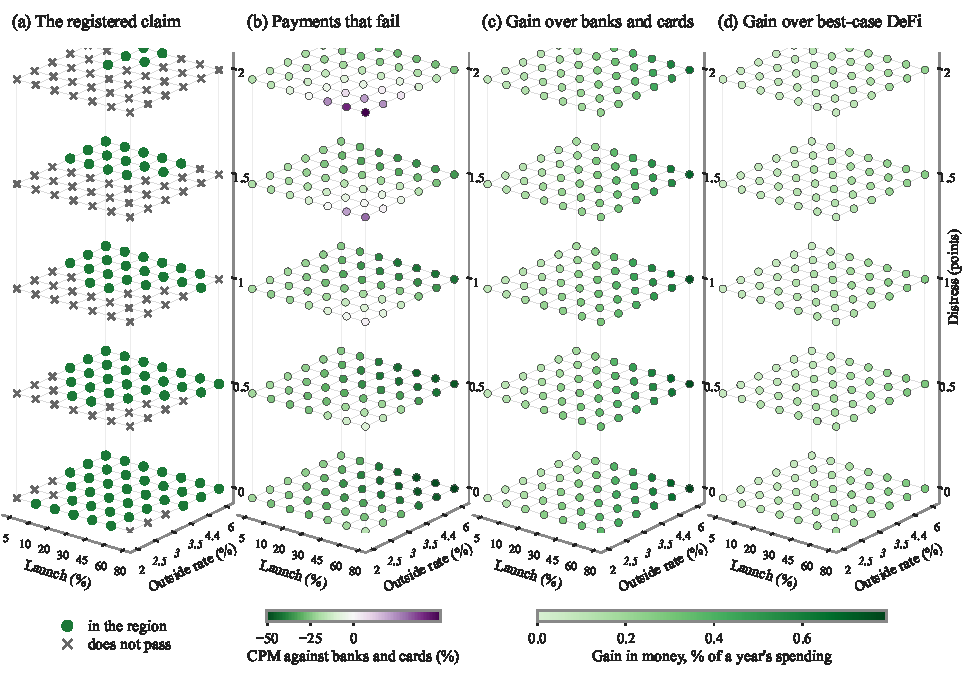
\includegraphics[width=\linewidth]{figures/fig_grid.pdf}
\caption{The whole experiment in the space of its three controls. Each marker is one cell: a launch participation,
an outside rate and a level of distress, read on its seeds; each layer is one level of distress. (a) The registered
claim: the cells in the region of their map. (b) CPM's share of payments that fail against that of banks and
cards, as a relative difference: green where CPM's is lower, purple where higher. (c) and (d) CPM's gain in
money over banks and cards and over best-case DeFi over the sixty months, as a share of a year's spending, on one
scale. The outside rates in italics, 2.5, 3 and 3.5\%, are the exploratory rate cut (Section~\ref{sec:lowrates}) on \CutSeeds{} seeds; the
others are the registered map on \NumSeeds{} seeds.}
\label{fig:grid}
\end{figure}

\subsection{Payments}

Table~\ref{tab:arrangements} and Figure~\ref{fig:failed} give the share of payments that fail: of the value of
bills and purchases due in years 4 and 5, the part not paid on its due day. Wages are counted
apart, below. With no distress the share is \FailBanksMean{} under banks and cards and
\FailDefiMean{} under best-case DeFi, against \FailPoolMean{} with the pool without the charge and \FailCpmMean{}
under CPM, as means over the \CellsNoDistress{} cells. CPM's share is \FailCutBanks{} below that of banks and
cards and \FailCutDefi{} below best-case DeFi's. The pool without the charge is already \FailCutPoolBanks{} below
banks and cards. On this measure the pool and its credit do most of the work; what demurrage adds is the
price of that credit and the cash kept ready for it (Section~\ref{sec:demurrage}). The gap to both
alternatives opens with launch participation, since only a participant can draw a bridge, and is present at
every outside rate. Best-case DeFi stays close to banks and cards at every level: it moves payments and pays a
yield but does nothing for a payer who is short.

Each person pays 58.3\% of its spending as a wage to another. A wage not paid on
its due date stays owed and is paid later, so it is recorded apart. Taking bills, purchases
and wages together, the value not paid on its first due date is \FailedValueBanks{} a person a year under banks
and cards and \FailedValueCpm{} under CPM. Wages paid late are \FailedWageShareBanks{} of it under banks and
cards and \FailedWageShareCpm{} under CPM; purchases lost are the rest. The unpaid value falls mostly on people without a
card: the \NoCardPeople{} who hold none are the payers of \NoCardFailedShareBanks{} of it
under banks and cards and \NoCardFailedShareCpm{} under CPM. Shortfalls in the model come from the timing of receipts and
payments and from job loss. Unexpected expenses are switched off in every run (Section~\ref{sec:model}), so they do
not drive the need for bridging.

\begin{table}[htbp]\centering\small
\resizebox{\linewidth}{!}{% Written by scripts/paper_numbers.py from confirmation_quote.
\begin{tabular}{lrrrrr}
\toprule
Arrangement & Failed, none (mean) & Failed, none (range) & Failed, 2 points (mean) & Failed, 2 points (range) & Purchases completed (\$ a person a year) \\
\midrule
Banks and cards & 3.641\% & 3.585\% to 3.691\% & 5.916\% & 5.757\% to 6.058\% & \$31{,}124 \\
Best-case DeFi & 3.530\% & 3.264\% to 3.630\% & 5.655\% & 5.156\% to 5.887\% & \$31{,}137 \\
Pool without the holding charge & 2.453\% & 1.968\% to 3.069\% & 4.968\% & 4.312\% to 6.654\% & \$31{,}424 \\
CPM & 2.373\% & 1.826\% to 2.997\% & 4.919\% & 4.204\% to 6.773\% & \$31{,}452 \\
Indexed CPM & 2.362\% & 1.816\% to 2.968\% & 4.893\% & 4.195\% to 6.645\% & \$31{,}454 \\
\bottomrule
\end{tabular}
}
\caption{Payments that fail: the value of bills and purchases not paid on their due day, as a share of the value
due in years 4 and 5 (wages counted apart), with no distress and at 2 points of distress, by
arrangement: the mean and the range over cells of the seed means. The last column is purchases completed.}
\label{tab:arrangements}
\end{table}

\begin{figure}[htbp]\centering
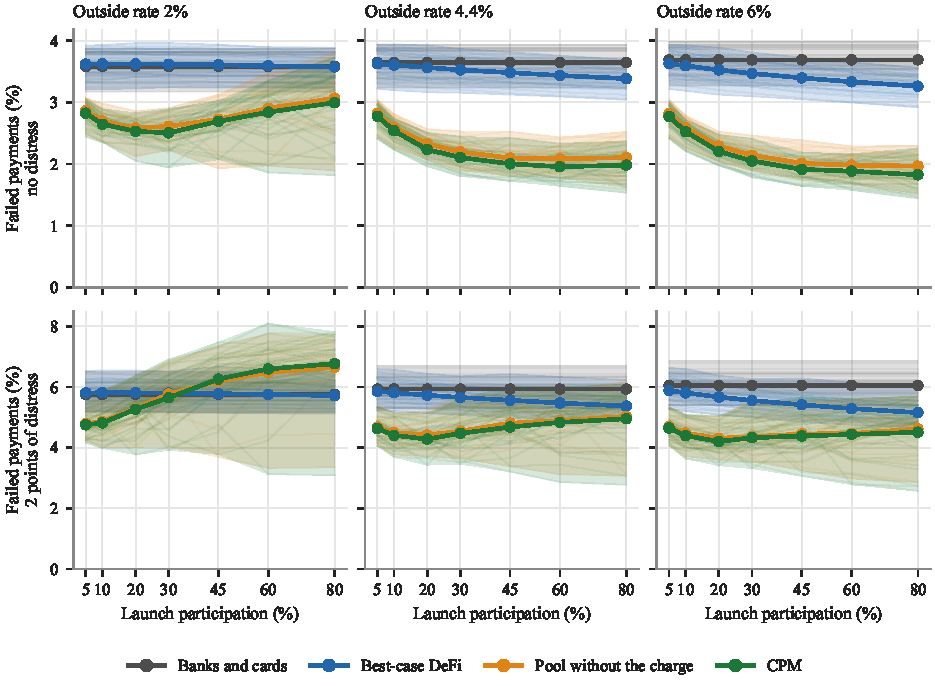
\includegraphics[width=\linewidth]{figures/fig_failed_payments.pdf}
\caption{Payments that fail against launch participation, by outside rate, with no distress (top) and at 2 points
of distress (bottom). Thick lines are seed means, bands the range of the seeds and thin lines the single seeds. Under
distress at high launch the seeds part, and the mean is the path of none of them.}
\label{fig:failed}
\end{figure}

\subsection{Gains}

Figure~\ref{fig:gains} and Table~\ref{tab:gains} give CPM's gain per person per year. A person in the model
stands for one United States consumer unit, so a figure per person is per household. Against banks and
cards the
median over cells is \GainBanksMedian{} in money alone and \GainBanksFaceMedian{} with completed purchases
counted at their price. Against best-case DeFi the two are \GainDefiMedian{} and \GainDefiFaceMedian{}. The
gain is positive in every cell at both ends of the bracket. It stays positive in every cell when the cash-advance
fees and interest CPM saves are taken out: the lowest cell then reads \GainBanksBoundLow{} against banks and
cards and \GainDefiBoundLow{} against best-case DeFi, in money alone. In
\CellsGainPositive{} of the \CellsAll{} cells, at every level of distress, CPM's mean gain over both
alternatives is positive in money alone, with completed purchases counted, and under the cash-advance bound.

The same result can be stated without dollars, which depend on the model's unit, a month of mean spending of
\$6,440. As a share of a year's spending the gain in money is \GainBanksSpending{} over banks and cards and
\GainDefiSpending{} over best-case DeFi, and \GainBanksFaceSpending{} and \GainDefiFaceSpending{} with completed
purchases at their price. A larger number is the change in what households pay intermediaries outside the
household economy, net of what those pay back: interest and the cash-advance and late fees of outside lenders,
failure fees, card fees less rewards, the spread banks and funds keep on balances and, under CPM, the issuer's custody, the pool's
operating cost and gas. At the median cell it is \OutsidePaidBanks{} a person a year under banks and cards,
\OutsidePaidDefi{} under best-case DeFi and \OutsidePaidCpm{} under CPM. Cell by cell CPM cuts it by a median of
\OutsideCutBanks{} against banks and cards, from \OutsideCutBanksLow{} at the lowest launch level to
\OutsideCutBanksHigh{} at the highest, and by \OutsideCutDefi{} against best-case DeFi. Without the spread on
balances, which is yield forgone and not cash paid, the cut against banks and cards is \OutsideCashCutBanks{}.
These payments are transfers, not resources used; the efficiency reading is the real cost below.

These are averages over people, and the average is above the typical person. In money alone the median person at
the median cell gains \PersonMedianBanks{} a year over banks and cards and \PersonMedianDefi{} over best-case
DeFi, \PersonMedianBanksSpending{} and \PersonMedianDefiSpending{} of a year's spending and less than half the
mean. At the fifth percentile the gain is \PersonFifthBanks{} and
\PersonFifthDefi{} a year. In money alone
\ShareBehindBanksMoney{} of people end more than \$2 a year behind the bank arrangement and
\ShareBehindDefiMoney{} behind best-case DeFi; with completed purchases at their price the shares are
\ShareBehindBanks{} and \ShareBehindDefi{} (Table~\ref{tab:gains}). The claim's group clause reads the mean of
each group, not each person.

In real resources CPM uses less than banks and cards in every cell, by at least \RealCostBanksLow{} a person a
year. Against best-case DeFi the difference is small in every cell, from \RealCostDefiLow{} to
\RealCostDefiHigh{} a person a year, with CPM using slightly more at the highest launch levels
(Table~\ref{tab:gains}). So the gain over best-case DeFi is the credit the pool supplies, apart from
0.20 point of yield on balances, which the custody check of Section~\ref{sec:robustness} removes without changing
the sign. It is not a cheaper way of moving money.

Two read-outs stored with the real cost say the same in other units. The model costs each payment the pool
rescues at \$2, as it does a failed one. CPM would use the same real resources as best-case DeFi if a rescue cost
between \RescueEvenDefiLow{} and \RescueEvenDefiHigh{} across the cells with no distress (median
\RescueEvenDefiMedian{}), and the same as banks and cards if it cost between \RescueEvenBanksLow{} and
\RescueEvenBanksHigh{} (median \RescueEvenBanksMedian{}). Against banks and cards the comparison has room to
spare; against best-case DeFi it rests on what a rescue is taken to cost. For each dollar of purchases completed
the real cost is \CentsCompletedBanks{} cents under banks and cards, \CentsCompletedDefi{} under best-case DeFi
and \CentsCompletedCpm{} under CPM, on average over the same cells.

\begin{figure}[htbp]\centering
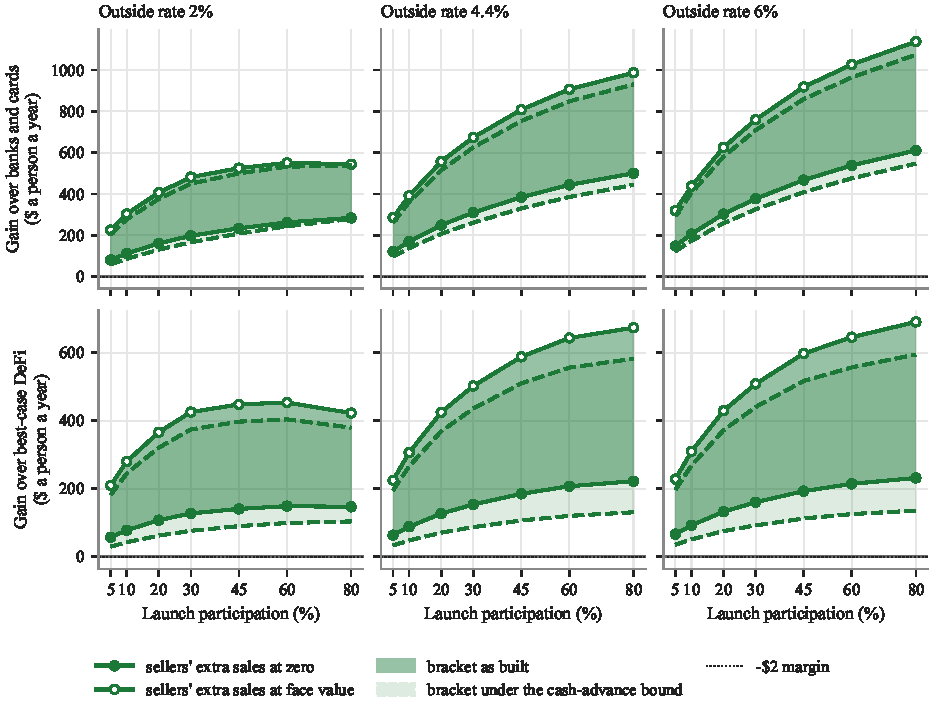
\includegraphics[width=\linewidth]{figures/fig_gains.pdf}
\caption{CPM's gain per person per year against banks and cards (top) and against best-case DeFi (bottom), by
outside rate, with no distress. The band runs from the gain in money alone to the gain with completed purchases at
their price; the dashed band is the same under the cash-advance bound.}
\label{fig:gains}
\end{figure}

\begin{table}[htbp]\centering\small
\resizebox{\linewidth}{!}{% Written by scripts/paper_numbers.py from confirmation_quote.
\begin{tabular}{lrrrr}
\toprule
 & Banks (median) & Banks (range) & DeFi (median) & DeFi (range) \\
\midrule
Wealth gain & \$262 & \$80 to \$610 & \$140 & \$57 to \$231 \\
Complete gain at face value & \$550 & \$225 to \$1{,}138 & \$429 & \$209 to \$690 \\
Complete gain at zero & \$262 & \$80 to \$610 & \$140 & \$57 to \$231 \\
Wealth gain under the cash-advance bound & \$243 & \$59 to \$547 & \$87 & \$29 to \$135 \\
Complete gain at face, under the bound & \$532 & \$204 to \$1{,}074 & \$379 & \$182 to \$594 \\
Complete gain at zero, under the bound & \$243 & \$59 to \$547 & \$87 & \$29 to \$135 \\
Cash-advance fees and interest saved & \$33 & \$5.3 to \$64 & \$51 & \$27 to \$96 \\
Real cost saved & \$18 & \$4.7 to \$40 & $-$\$0.1 & $-$\$2.0 to \$0.2 \\
Share below $-$\$2 a year, complete gain at face & 10.6\% & 9.2\% to 17.7\% & 13.2\% & 11.5\% to 20.3\% \\
Wealth gain read at month 36 & \$221 & \$45 to \$560 & \$114 & \$30 to \$208 \\
Wealth gain read at month 48 & \$263 & \$61 to \$589 & \$135 & \$42 to \$221 \\
\midrule
Lowest group lower bound, as built & \multicolumn{4}{l}{\$0.5} \\
Lowest group lower bound, under the bound & \multicolumn{4}{l}{$-$\$2.6} \\
\midrule
Clause (a) & \multicolumn{4}{l}{21 of 21} \\
Clause (b) & \multicolumn{4}{l}{20 of 21} \\
Clause (c), reported & \multicolumn{4}{l}{21 of 21} \\
Clause (d) as built & \multicolumn{4}{l}{21 of 21} \\
Clause (d) under the bound & \multicolumn{4}{l}{20 of 21} \\
All of (a), (b), (d) as built & \multicolumn{4}{l}{20 of 21} \\
All of (a), (b), (d) under the bound & \multicolumn{4}{l}{19 of 21} \\
All, as built and under the bound & \multicolumn{4}{l}{19 of 21} \\
In the region (largest joined block) & \multicolumn{4}{l}{19 of 21} \\
\bottomrule
\end{tabular}
}
\caption{CPM against banks and cards and against best-case DeFi over the \CellsNoDistress{} cells with no distress,
in dollars a person a year: median and range over cells. The lower block counts the cells where each clause of
the registered claim passes on the \NumSeeds{} confirmation seeds.}
\label{tab:gains}
\end{table}

\subsection{Where the gain comes from}

Table~\ref{tab:sources} splits CPM's gain in money over banks and cards by the flow it comes from, at each outside
rate with no distress. The split is an accounting identity: in every cell its lines add up to the gain. Four lines
carry it. The reserve return paid on P is \SourceYieldTwo{} a person a year at an outside rate of 2\%,
\SourceYieldFourFour{} at 4.4\% and \SourceYieldSix{} at 6\%, or \SourceYieldShareTwo{},
\SourceYieldShareFourFour{} and \SourceYieldShareSix{} of the gain. Interest no longer paid to cards and outside
lenders, because the pool lent instead and its interest stays with the households that own it, is
\SourceInterestTwo{}, \SourceInterestFourFour{} and \SourceInterestSix{}, or \SourceInterestShareTwo{},
\SourceInterestShareFourFour{} and \SourceInterestShareSix{} of the gain. Cash-advance, late and failure fees saved are \SourceFeesTwo{},
\SourceFeesFourFour{} and \SourceFeesSix{}, and card fees saved, less the rewards given up, about
\SourceCardFourFour{} at every rate. Against them stand the pool's operating cost and the savings income given up
on money moved into P and the pool.

The reserve return moves most with the outside rate; the fees saved also nearly double between 2\% and 4.4\%. Best-case DeFi also pays its holders a return on the
reserve and moves money off the card rails, so of these lines the two that come from credit, the interest and the
fees saved, separate CPM from it. That is why the gain over best-case DeFi is the smaller of the two and
changes less with the outside rate (Figure~\ref{fig:gains}). The reserve return is also one of the two reasons the
claim is weakest at low outside rates (Section~\ref{sec:lowrates}).

\begin{table}[htbp]\centering\small
% Written by scripts/paper_numbers.py from confirmation_quote.
\begin{tabular}{lrrr}
\toprule
Outside rate & 2.0\% & 4.4\% & 6.0\% \\
\midrule
Reserve return on P and other outside income & \$55 & \$138 & \$194 \\
Interest saved on outside loans & \$102 & \$118 & \$133 \\
Card fees saved, less rewards given up & \$41 & \$42 & \$42 \\
Cash-advance, late and failure fees saved & \$34 & \$65 & \$69 \\
The pool's operating cost & $-$\$22 & $-$\$17 & $-$\$17 \\
Savings income given up, inflation and valuation & $-$\$22 & $-$\$35 & $-$\$43 \\
Conversion fees, gas and wages to the outside & $-$\$1.8 & $-$\$1.6 & $-$\$1.6 \\
\midrule
Gain over banks and cards & \$197 & \$309 & \$376 \\
\bottomrule
\end{tabular}

\caption{CPM's gain in money over banks and cards by the flow it comes from, in dollars a person a year: the median
over the seven launch levels at each outside rate, with no distress. The lines add up to the gain in each cell;
medians over cells need not add up exactly.}
\label{tab:sources}
\end{table}

Figure~\ref{fig:sources} gives the same split in every cell, in dollars and as shares of the cell's gain. As launch
participation rises, card fees saved take a larger share of the gain and the fees saved on shortfalls a smaller
one; the shares of the reserve return and of the interest move less.

\begin{figure}[htbp]\centering
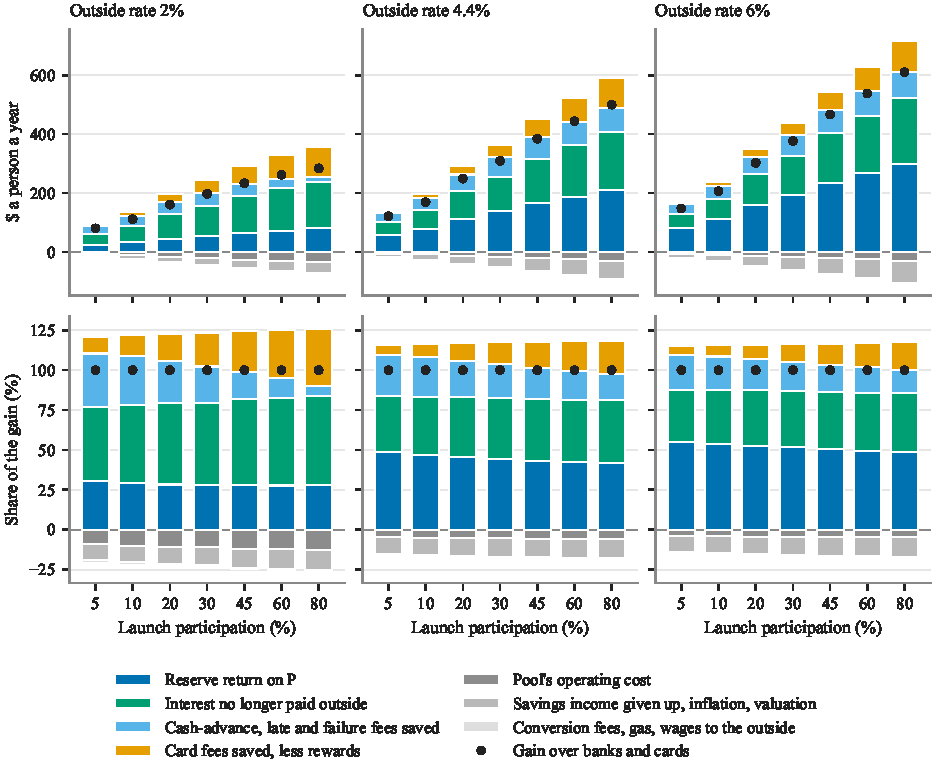
\includegraphics[width=\linewidth]{figures/fig_sources.pdf}
\caption{CPM's gain in money over banks and cards by the flow it comes from, in each of the \CellsNoDistress{} cells
with no distress: dollars a person a year (top) and each flow as a share of the cell's gain (bottom). Costs are
stacked below zero and the dot marks the gain.}
\label{fig:sources}
\end{figure}

\subsection{What demurrage does}\label{sec:demurrage}

The pool without the charge is the same money and the same pool on the same people and draws, so its difference
from CPM is what demurrage does (Tables~\ref{tab:buys} and~\ref{tab:charge}, Figure~\ref{fig:charge}).

The demurrage rate is \ChargeFrom{} to \ChargeTo{} a year across cells. At the median cell the holding charge costs holders
\ChargeDollars{} a person a year, and Table~\ref{tab:buys} sets beside that cost what it pays for. The price a
bridge borrower pays falls from between \BridgePricePoolLow{} and \BridgePricePoolHigh{}, depending on the outside
rate, to \BridgePriceCpm{} at every rate, a cut of \BridgeCutLow{} to \BridgeCutHigh{}, as
equation~\eqref{eq:bridgeprice} requires: the capital part of the coupon moves from the borrower to all holders.
The pool keeps \StandbyChange{} more cash standing by, \StandbyCpm{} a person against \StandbyPool{}, because its
capital target now includes cash against the peak of bridging, and serves a larger share of the bridges asked
of it at every outside rate. Bridging by the pool rises by \PoolBridgingChange{}, from \PoolBridgingPool{} to
\PoolBridgingCpm{} a person a year. Balances revolved on cards fall by \RevolvedChange{}, from \RevolvedPool{} to
\RevolvedCpm{}, and the value of payments that fail from \FailedDollarsPool{} to \FailedDollarsCpm{}.

By Corollary~\ref{cor:neutral} the charge cannot create wealth at fixed quantities: what holders pay, borrowers
and owners receive. So CPM's net gain over the pool without the charge is the value of the quantities
that changed. At the median cell it is \GainOverPool{} a person a year over the whole run and
\GainOverPoolLate{} in years 4 and 5, when the charge collected is \ChargeDollars{}: household
wealth is \GainPerChargeDollar{} dollars higher for each dollar collected. That compares two runs; it is not
a payment the contract makes. The size check (Section~\ref{sec:robustness}) shows the gain still grows
with the population. Demurrage here is insurance
and is priced like it: a small premium on every balance, paid out as cheap and available credit to whoever
is short.

In dollars this is the smallest gain the paper reports, so it is read with its interval. CPM and the pool without
the charge run on the same people and draws, and their difference is paired seed by seed.
Table~\ref{tab:chargegain} and Figure~\ref{fig:chargegain} give it at every distress level (Section~\ref{sec:stress}). Under the quote rule, where savers enter on the
pool's published quote, the median over cells is
\ChargeGainFirstMedianZero{} a person a year with no distress and \ChargeGainFirstMedianTwo{} at 2 points. The
lower end of the 95\% interval across seeds is above zero in \ChargeGainFirstAboveAll{} of the
\ChargeGainFirstCells{} cells of the grid; the lowest, at 2 points, is \ChargeGainFirstLowTwo{}. CPM fails fewer
payments than the pool without the charge in \ChargeGainFirstFewerAll{} of those cells. Under the record rule,
where they enter on its realised return (Section~\ref{sec:record}), the medians are \ChargeGainSecondMedianZero{} and
\ChargeGainSecondMedianTwo{}, the lower end is above zero in \ChargeGainSecondAboveAll{} cells and CPM fails fewer
payments in \ChargeGainSecondFewerAll{}. These intervals are not part of the registered claim and carry no
correction for the number of cells.

\begin{table}[htbp]\centering\small
\resizebox{\linewidth}{!}{% Written by scripts/paper_numbers.py from confirmation_quote.
\begin{tabular}{lrrrrrrrr}
\toprule
 & \multicolumn{4}{c}{Quote rule} & \multicolumn{4}{c}{Record rule} \\
Distress & Median gain & Lowest lower bound & Cells above zero & Cells with fewer failures & Median gain & Lowest lower bound & Cells above zero & Cells with fewer failures \\
\midrule
0 pt & \$15 & \$4.9 & 21 & 21 & \$61 & \$34 & 21 & 21 \\
0.5 pt & \$15 & \$4.7 & 21 & 21 & \$56 & \$35 & 21 & 21 \\
1 pt & \$13 & \$4.6 & 21 & 19 & \$53 & \$32 & 21 & 19 \\
1.5 pt & \$13 & \$3.8 & 21 & 18 & \$50 & \$27 & 21 & 18 \\
2 pt & \$12 & \$0.1 & 21 & 18 & \$46 & \$21 & 21 & 15 \\
\bottomrule
\end{tabular}
}
\caption{CPM's gain in money over the pool without the charge, in dollars a person a year, by distress level and
under the two entry rules: the median over the \CellsNoDistress{} cells of each level; the lowest,
over those cells, of the lower end of the 95\% interval of the paired gain across the \NumSeeds{} seeds; the cells
where that lower end is above zero; and the cells where CPM fails fewer payments than the pool without the
charge.}
\label{tab:chargegain}
\end{table}

\begin{figure}[htbp]\centering
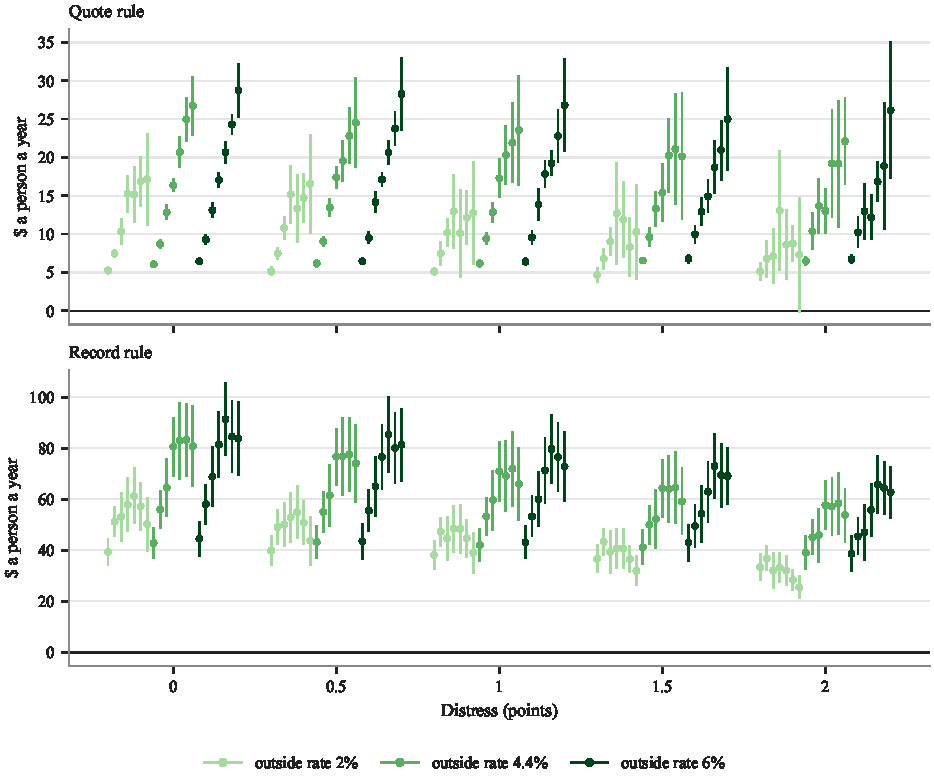
\includegraphics[width=\linewidth]{figures/fig_charge_gain.pdf}
\caption{CPM's gain in money over the pool without the charge in every cell of the grid: the mean across the
\NumSeeds{} seeds and its 95\% interval, by distress level, under the quote rule (top) and the record rule
(bottom). Within a level the cells run by outside rate and then by launch participation.}
\label{fig:chargegain}
\end{figure}

Table~\ref{tab:buys} also measures liquidity support across arrangements. Banks and cards hold \PrecautionBanks{} dollars of
precautionary money for each dollar of shortfall a lender covers in a year, and best-case DeFi \PrecautionDefi{}.
The pool holds \PrecautionPool{} without the charge and \PrecautionCpm{} with it, and covers more shortfalls than
either. Each dollar of precautionary money covers more shortfall once part of it is pooled; households' own
buffers are no smaller (Table~\ref{tab:buys}).

\begin{table}[htbp]\centering\small
\resizebox{\linewidth}{!}{% Written by scripts/paper_numbers.py from confirmation_quote.
\begin{tabular}{lrrrr}
\toprule
 & Banks and cards & Best-case DeFi & Pool without the holding charge & CPM \\
\midrule
Demurrage paid by holders, \$ a person a year &  &  & \$0.0 & \$4.7 \\
Bridge price to the borrower, \% a year &  &  & 6.7\% & 2.1\% \\
Shortfalls a lender covered, \$ a person a year & \$2{,}783 & \$3{,}119 & \$4{,}879 & \$5{,}015 \\
\quad by the pool & \$0.0 & \$0.0 & \$2{,}645 & \$2{,}982 \\
\quad on the card & \$1{,}868 & \$2{,}198 & \$1{,}407 & \$1{,}357 \\
\quad revolved on the card & \$872 & \$907 & \$706 & \$637 \\
Payments that failed, \$ a person a year & \$3{,}042 & \$3{,}006 & \$2{,}147 & \$2{,}094 \\
Precautionary money held, \$ a person & \$1{,}289 & \$1{,}726 & \$1{,}740 & \$1{,}742 \\
\quad of which pool cash standing by & \$0.0 & \$0.0 & \$31 & \$50 \\
Precautionary money per dollar of shortfall covered & 0.46 & 0.54 & 0.36 & 0.36 \\
Gain over the pool without the charge, \$ a person a year &  &  &  & \$15 \\
\bottomrule
\end{tabular}
}
\caption{What demurrage buys, and liquidity support by arrangement: medians over the cells with no
distress, years 4 and 5. A shortfall is what a payer's own money and same-day savings could not pay; a lender
covers it through the pool, the card, a balance revolved on the card or earned-wage access. Precautionary money
is households' chosen buffers and the pool's idle cash.}
\label{tab:buys}
\end{table}

\begin{table}[htbp]\centering\small
\resizebox{\linewidth}{!}{% Written by scripts/paper_numbers.py from confirmation_quote.
\begin{tabular}{llrrrrrrr}
\toprule
Outside rate & Arrangement & Bridge price & Gross coupon & Bridges served & Demurrage $c$ & $\theta$ & Payments that fail & Gain over the pool without the charge \\
\midrule
2.0\% & Pool without the holding charge & 4.34\% & 4.34\% & 0.675 & 0.000\% & 0.000 & 2.728\% &  \\
2.0\% & CPM & 2.10\% & 4.34\% & 0.758 & 0.070\% & 0.518 & 2.693\% & \$15 \\
4.4\% & Pool without the holding charge & 6.75\% & 6.75\% & 0.792 & 0.000\% & 0.000 & 2.198\% &  \\
4.4\% & CPM & 2.09\% & 6.74\% & 0.872 & 0.137\% & 0.690 & 2.106\% & \$16 \\
6.0\% & Pool without the holding charge & 8.34\% & 8.34\% & 0.800 & 0.000\% & 0.000 & 2.144\% &  \\
6.0\% & CPM & 2.08\% & 8.33\% & 0.880 & 0.177\% & 0.750 & 2.051\% & \$17 \\
\bottomrule
\end{tabular}
}
\caption{CPM against the pool without the charge, with no distress, by outside rate: medians over launch levels of
the seed means in years 4 and 5.}
\label{tab:charge}
\end{table}

\begin{figure}[htbp]\centering
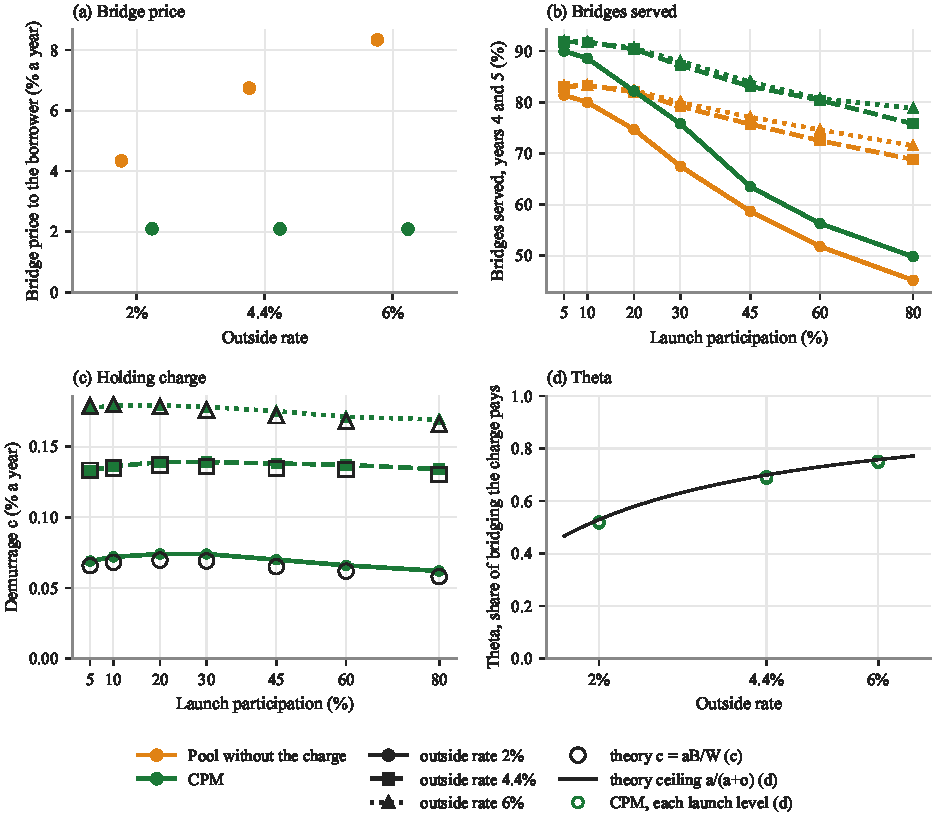
\includegraphics[width=\linewidth]{figures/fig_charge.pdf}
\caption{What demurrage does. (a) The price a bridge borrower pays. (b) Bridges served. (c) The charge,
with the value $a\,B/W$ of Proposition~\ref{prop:size} where the stored fields allow. (d) The charge's share of
bridging finance against its ceiling $a/(a+o)$.}
\label{fig:charge}
\end{figure}

\subsection{Circulation}

The arrangement's name invites a question its mechanism does not depend on: whether a charge on balances makes
money move faster. We measure circulation with MicroVelocity \cite{campajola} in years 4 and 5
(Table~\ref{tab:circulation}, Figure~\ref{fig:circulation}). A unit of money held for $\tau$ days between
receipt and spending adds $1/\tau$ for each day it is held; a person's MicroVelocity is that sum over the
money it holds, divided by the total stock of money, so people's MicroVelocities add up to the velocity of
money. Money spent is matched to money received last in first out, as in \cite{decollibus}, with first in first
out beside it, and money not spent again within the run is left out, as in both papers. Wallet turnover is
also reported: a person's payments to others over a year divided by its own average balance of bank money
and $P$, the inverse of its average holding time. The time between
receipt and spending is the holding time of \cite{campajola}; \cite{zhang} call it the lifespan.

Gesell's demurrage \cite{gesell} was meant to make money circulate faster. This one does not speed circulation by
any amount that matters. Under CPM the money a participant spends has been
held for \HoldingDaysCpm{} days on average, against \HoldingDaysPool{} days in the pool without the charge, and the
velocity of all money is \VelocityCpm{} turns a year against \VelocityPool{}. The differences have a consistent
sign and are about one per cent. The size of the charge implies as much: a fraction of a percentage
point a year gives nobody a reason to spend sooner. The demurrage works through the price and availability of
bridging, as Section~\ref{sec:implications} derives, not through the speed of spending.

The pool, with or without the charge, does change the measure. The velocity of all money is \VelocityBanks{} turns
a year under banks and cards and \VelocityDefi{} under best-case DeFi, against \VelocityCpm{} under CPM. The measure counts bank money, $P$ and
outside savings. Spare money placed in the pool is lent on and spent, where spare money in outside savings
sits, so a smaller stock of money carries the same spending. The rise reflects where spare money rests,
not people spending faster. Circulation is no more concentrated under the pool: the tenth of
people who contribute most to velocity carry about a quarter of it in every arrangement.

\begin{table}[htbp]\centering\footnotesize
\resizebox{\linewidth}{!}{% Written by scripts/paper_numbers.py from confirmation_quote.
\begin{tabular}{lllllrr}
\toprule
 & Statistic & Unit & Arrangement & People & Median & Range \\
\midrule
(a) & Wallet turnover, median person & turns a year & Banks and cards & everyone & 49.6 & 48.5 to 49.9 \\
 &  &  & Best-case DeFi & participants & 19.8 & 18.7 to 20.0 \\
 &  &  & Pool without the holding charge & participants & 24.0 & 22.5 to 27.8 \\
 &  &  & CPM & participants & 24.0 & 22.6 to 28.1 \\
\midrule
(a) & Wallet turnover, balance-weighted mean & turns a year & Banks and cards & everyone & 47.6 & 46.6 to 47.9 \\
 &  &  & Best-case DeFi & participants & 13.4 & 12.7 to 13.7 \\
 &  &  & Pool without the holding charge & participants & 15.7 & 15.2 to 18.3 \\
 &  &  & CPM & participants & 15.8 & 15.3 to 18.5 \\
\midrule
(b) & MicroVelocity, top tenth's share of the group's sum & share & Banks and cards & everyone & 0.255 & 0.254 to 0.255 \\
 &  &  & Best-case DeFi & participants & 0.242 & 0.237 to 0.246 \\
 &  &  & Pool without the holding charge & participants & 0.244 & 0.243 to 0.245 \\
 &  &  & CPM & participants & 0.243 & 0.243 to 0.246 \\
\midrule
(b) & MicroVelocity, median person & turns a year & Banks and cards & everyone & 0.00201 & 0.00199 to 0.00203 \\
 &  &  & Best-case DeFi & participants & 0.00238 & 0.00225 to 0.00269 \\
 &  &  & Pool without the holding charge & participants & 0.00251 & 0.00226 to 0.00314 \\
 &  &  & CPM & participants & 0.00253 & 0.00227 to 0.00315 \\
\midrule
(b) & Aggregate velocity, MicroVelocity summed over everyone & turns a year & Banks and cards & everyone & 10.32 & 10.18 to 10.41 \\
 &  &  & Best-case DeFi & everyone & 10.64 & 10.46 to 11.44 \\
 &  &  & Pool without the holding charge & everyone & 12.48 & 11.07 to 15.57 \\
 &  &  & CPM & everyone & 12.54 & 11.13 to 15.76 \\
\midrule
(c) & Mean holding time of money spent, last in first out & days & Banks and cards & everyone & 26.5 & 26.2 to 26.7 \\
 &  &  & Best-case DeFi & participants & 29.5 & 27.2 to 31.9 \\
 &  &  & Pool without the holding charge & participants & 27.2 & 22.9 to 29.8 \\
 &  &  & CPM & participants & 26.9 & 22.5 to 29.6 \\
\midrule
(c) & Mean holding time of money spent, first in first out & days & Banks and cards & everyone & 34.9 & 34.6 to 35.3 \\
 &  &  & Best-case DeFi & participants & 33.8 & 33.6 to 35.2 \\
 &  &  & Pool without the holding charge & participants & 27.4 & 22.7 to 29.8 \\
 &  &  & CPM & participants & 27.2 & 22.4 to 29.6 \\
\bottomrule
\end{tabular}
}
\caption{Circulation in years 4 and 5 with no distress, by arrangement: median and range over cells of the seed
means. Wallet turnover is a person's outflow over its own average balance of bank money and $P$. MicroVelocity and
holding times are computed from the age of every unit of bank money, $P$ and outside savings when it is spent.
Banks and cards have no network, so their rows cover everyone; the other rows cover each arrangement's
participants unless marked.}
\label{tab:circulation}
\end{table}

\begin{figure}[htbp]\centering
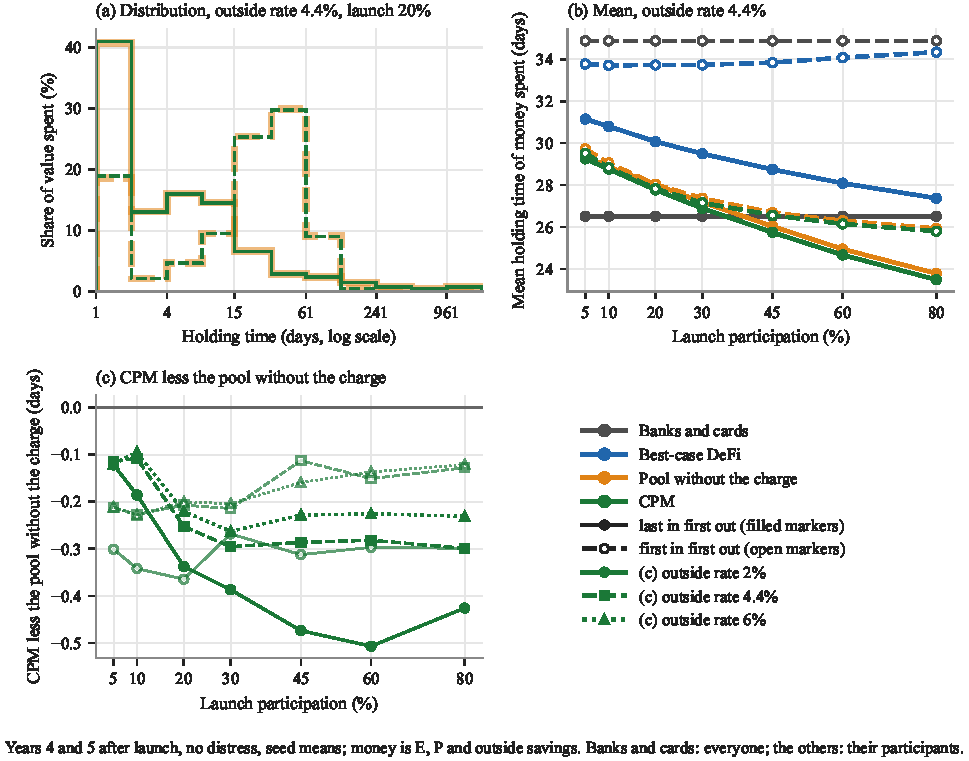
\includegraphics[width=\linewidth]{figures/fig_circulation.pdf}
\caption{Holding times of money spent, years 4 and 5, no distress. (a) The distribution of value spent by holding
time under CPM and under the pool without the charge at one cell. (b) The mean holding time against launch
participation at an outside rate of 4.4\%. (c) CPM less the pool without the charge. Filled markers count the
newest money as spent first, open markers the oldest.}
\label{fig:circulation}
\end{figure}

\subsection{Theory against simulation}

Table~\ref{tab:docking} sets the equations of Section~\ref{sec:implications} beside the simulation over the cells
with no distress, with the largest gap in any cell; its last column says how each row holds. Four rows hold by
construction. The simulation computes the charge, the bridge price and the quote by the contract's own equations,
and the charge's share of bridging finance is a ratio of recorded flows the coupon fixes. These rows check
that the code runs the contract as written and that its records add up. Their value is the size of the
numbers: the charge of Proposition~\ref{prop:size}, computed from the bridge book and wallet balances without its
small standby term, matches the simulated charge, and the share follows Proposition~\ref{prop:theta}. The other
rows predict behaviour. Participation follows the one curve of Proposition~\ref{prop:diffusion}
from every launch level with one fitted leaving rate (Figure~\ref{fig:participation}).

One prediction holds only in part. Proposition~\ref{prop:capital} puts capital at its target when the money offered
exceeds the room. With savers reviewing entry at the monthly rate, offers do not always fill the room, and in the
worst cell capital is below 95\% of its target in the share of seed-months given in the fourth row of
Table~\ref{tab:docking}. The proposition's condition is real, not a formality. Its other half, that
entrants act on the quote, is taken up in Section~\ref{sec:record}.

Proposition~\ref{prop:fair} says the quote is right on average and that an owner's shortfall is a loss tail. Both show.
Owners earn their alternative at the median, with a tail below it. Table~\ref{tab:owners} gives the realised
return on pool capital less the alternative in years 4 and 5 over the seed-cells with no distress. At every
outside rate the median is within \OwnersMedianWorst{} of a percentage point of zero. In one seed-cell in ten
owners fall short of their alternative by \OwnersTenthLeast{} to \OwnersTenthWorst{} of a point a year or more,
depending on the outside rate. The tail matters, because an owner decides whether to stay on its realised
return (Section~\ref{sec:entry}).

\begin{table}[htbp]\centering\small
\resizebox{\linewidth}{!}{% Written by scripts/paper_numbers.py from confirmation_quote.
\begin{tabular}{lrrrl}
\toprule
Quantity & Formula & Simulated & Largest gap & Holds \\
\midrule
Demurrage rate $c = aB/W$ (the standby part $(a - p)S/W$ is not stored), \% a year & 0.058\% to 0.180\% & 0.062\% to 0.179\% & 0.005\% & by construction \\
$\theta = a / r_g$ & 0.517 to 0.751 & 0.517 to 0.751 & 0.002 & by construction \\
Bridge price $= r_g - \kappa a$, \% a year & 2.07\% to 2.12\% & 2.07\% to 2.12\% & 0.00\% & by construction \\
Seed-months with capital below 0.95 of its target & 0.000 & 0.001 to 0.538 & 0.538 & in part \\
Quote at the target $= a$, \% a year & 2.25\% to 6.25\% & 2.24\% to 6.25\% & 0.01\% & by construction \\
Participation at month 12 & 0.098 to 0.853 & 0.099 to 0.849 & 0.014 & as predicted \\
Participation at month 36 & 0.251 to 0.927 & 0.252 to 0.928 & 0.010 & as predicted \\
Participation at month 60 & 0.458 to 0.963 & 0.457 to 0.966 & 0.023 & as predicted \\
\bottomrule
\end{tabular}
}
\caption{Theory against simulation over CPM's cells with no distress: each quantity's formula value and the
simulated value, as ranges over cells, and the largest gap in any cell. A row holds by construction where the
simulation computes the quantity by that equation, as predicted where the equation describes behaviour, and in
part where the prediction's condition is not always met.}
\label{tab:docking}
\end{table}

\begin{figure}[htbp]\centering
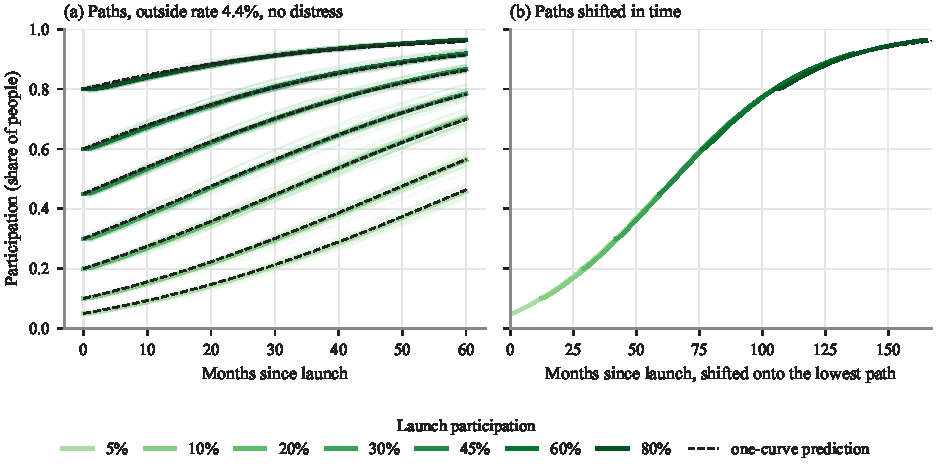
\includegraphics[width=\linewidth]{figures/fig_participation.pdf}
\caption{Participation under CPM at an outside rate of 4.4\% with no distress. (a) Paths from the seven launch
levels, the seed mean thick and each seed thin, with the prediction of equation~\eqref{eq:diffusion}. (b) The
seed-mean paths shifted in time onto the path from the lowest launch level.}
\label{fig:participation}
\end{figure}

\begin{table}[htbp]\centering\small
% Written by scripts/paper_numbers.py from confirmation_quote.
\begin{tabular}{lrrrr}
\toprule
Outside rate & Median & Mean & 10th percentile & Seed-cells with capital \\
\midrule
2.0\% & $-$0.01\% & 0.00\% & $-$0.31\% & 210 of 210 \\
4.4\% & $-$0.01\% & $-$0.09\% & $-$0.52\% & 210 of 210 \\
6.0\% & $-$0.02\% & $-$0.09\% & $-$0.51\% & 210 of 210 \\
\bottomrule
\end{tabular}

\caption{Owners' realised return less their alternative in years 4 and 5, in percentage points a year, over the
seed-cells with no distress.}
\label{tab:owners}
\end{table}

\subsection{The registered claim}

Table~\ref{tab:region} and Figure~\ref{fig:region} give the claim as registered, read once on the \NumSeeds{}
confirmation seeds. With no distress \ClaimCellsAsBuilt{} of the \CellsNoDistress{} cells pass clauses (a), (b) and
(d) as built, and \ClaimCellsBoth{} pass also under the cash-advance bound. Those cells join edge to edge, so the
region is one block of \RegionCellsZero{} cells: every cell at outside rates of 4.4\% and 6\%, and five of the
seven at 2\%. At the Bonferroni level over the \CellsNoDistress{} cells the claim holds in \ClaimHoldsSomewhere{}.
A falsifier fires in \ClaimCellsFalsified{} cell. The seed-count rule marks \ClaimCellsUnderpowered{} cell
underpowered: on the confirmation map's own spreads no cell needs more than \ClaimSeedsCellMost{} seeds, so the
declared extension to \SeedsExtended{} seeds is not used.

In every seed of every cell of the grid the pool forms, households hold at least 90\% of its capital through the
second window and the issuer stays. With no distress at least \SeedsPersistentLeast{} of the \NumSeeds{} seeds are Persistent in every
cell, and clause (a) passes in all of them (Table~\ref{tab:gains}).

The group clause decides little. Against best-case DeFi, with completed purchases at their price, the lowest lower
bound of any group in any cell is \GroupLowDefiFace{} a person a year as built and \GroupLowDefiFaceBound{} under
the bound: every group is ahead of best-case DeFi on the registered clause, by a wide margin. Against banks and
cards the clause is also read at the other end of the bracket, the group's gain in wealth plus the purchases it
received less its own extra sales, so with a seller's extra sales valued at nothing. For a group that is not its
gain in money alone. There the lowest is \GroupLowBanksZero{} as built and \GroupLowBanksZeroBound{} under the
bound, both at an outside rate of 2\% and a launch of 5\%. The second lies sixty cents beyond the \$2 margin, and
that cell is one of the two that miss. Its group means are positive; it misses on the lower end of an interval.

The other cell that misses is at an outside rate of 2\% and a launch of 80\%, on the real-cost clause. There the
real resources CPM saves against best-case DeFi are \RealCostDefiLow{} a person a year, at the margin itself, and
the interval reaches past it. Neither cell reads falsified: in both the interval straddles the margin. They are the
edge of the region and are reported as such.

Indexed CPM is read separately, in the \IndexedValid{} cells where it is defined. With no distress it is in its
region in \IndexedRegionZero{} of them and holds at its Bonferroni level in \IndexedHolds{}. Under distress its
region holds \IndexedRegionHalf{} cells at half a point, \IndexedRegionOne{} at 1 point, \IndexedRegionOneHalf{} at
1.5 points and \IndexedRegionTwo{} at 2 points, against \RegionCellsHalf{}, \RegionCellsOne{},
\RegionCellsOneHalf{} and \RegionCellsTwo{} for CPM, whose region under distress also lies at 4.4\% and 6\% only (Section~\ref{sec:stress}). Indexed CPM's
median gain over its \IndexedValid{} cells is \IndexedGainBanks{} a person a year over banks and cards and \IndexedGainDefi{} over best-case DeFi, where
CPM's is \IndexedCpmGainBanks{} and \IndexedCpmGainDefi{}. At 2\% inflation, stating the contract in
purchasing-power terms leaves the result unchanged.

\begin{table}[htbp]\centering\small
% Written by scripts/paper_numbers.py from confirmation_quote.
\begin{tabular}{llcccccccr}
\toprule
Distress & Outside rate & 5\% & 10\% & 20\% & 30\% & 45\% & 60\% & 80\% & Cells in region \\
\midrule
0 pt & 2.0\% & $\times$ & $\bullet$ & $\bullet$ & $\bullet$ & $\bullet$ & $\bullet$ & $\times$ & 19 \\
 & 4.4\% & $\bullet$ & $\bullet$ & $\bullet$ & $\bullet$ & $\bullet$ & $\bullet$ & $\bullet$ &  \\
 & 6.0\% & $\bullet$ & $\bullet$ & $\bullet$ & $\bullet$ & $\bullet$ & $\bullet$ & $\bullet$ &  \\
0.5 pt & 2.0\% & $\times$ & $\times$ & $\times$ & $\times$ & $\times$ & $\times$ & $\times$ & 14 \\
 & 4.4\% & $\bullet$ & $\bullet$ & $\bullet$ & $\bullet$ & $\bullet$ & $\bullet$ & $\bullet$ &  \\
 & 6.0\% & $\bullet$ & $\bullet$ & $\bullet$ & $\bullet$ & $\bullet$ & $\bullet$ & $\bullet$ &  \\
1 pt & 2.0\% & $\times$ & $\times$ & $\times$ & $\times$ & $\times$ & $\times$ & $\times$ & 13 \\
 & 4.4\% & $\bullet$ & $\bullet$ & $\bullet$ & $\bullet$ & $\bullet$ & $\bullet$ & $\bullet$ &  \\
 & 6.0\% & $\bullet$ & $\bullet$ & $\bullet$ & $\bullet$ & $\bullet$ & $\bullet$ & $\times$ &  \\
1.5 pt & 2.0\% & $\times$ & $\times$ & $\times$ & $\times$ & $\times$ & $\times$ & $\times$ & 10 \\
 & 4.4\% & $\bullet$ & $\bullet$ & $\bullet$ & $\bullet$ & $\bullet$ & $\times$ & $\times$ &  \\
 & 6.0\% & $\bullet$ & $\bullet$ & $\bullet$ & $\bullet$ & $\bullet$ & $\times$ & $\times$ &  \\
2 pt & 2.0\% & $\times$ & $\times$ & $\times$ & $\times$ & $\times$ & $\times$ & $\times$ & 4 \\
 & 4.4\% & $\times$ & $\times$ & $\bullet$ & $\bullet$ & $\times$ & $\times$ & $\times$ &  \\
 & 6.0\% & $\times$ & $\times$ & $\bullet$ & $\bullet$ & $\times$ & $\times$ & $\times$ &  \\
\bottomrule
\end{tabular}

\caption{The registered claim on the \NumSeeds{} confirmation seeds, by distress level, outside rate (rows) and
launch participation (columns): $\bullet$ in the region, $\circ$ passing outside the largest joined block,
$\times$ not passing. A cell at a level of distress is in the region when its cell with no distress passes and
withstands every level up to that one. The last column counts the cells in the region at each level.}
\label{tab:region}
\end{table}

\begin{figure}[htbp]\centering
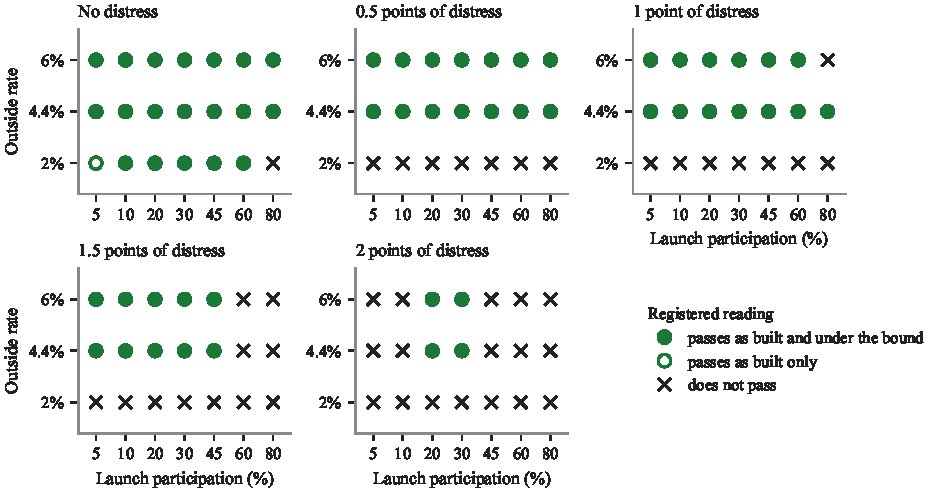
\includegraphics[width=\linewidth]{figures/fig_region.pdf}
\caption{The registered claim on the \NumSeeds{} confirmation seeds, one panel per distress level.}
\label{fig:region}
\end{figure}

\subsection{The edge at low outside rates}\label{sec:lowrates}

The registered grid has three outside rates, and the sharpest change in the claim lies between two of them: under
distress the region holds no cell at 2\% and, at half a point, every cell at 4.4\%. After the confirmation map was
read the gap was filled with a rate cut, outside rates of 2.5, 3 and 3.5\% over the same launch and distress
levels, on the frozen model and read by the same rules. It is exploratory. It was run on \CutSeedsTried{} seeds
of a block kept for runs after the confirmation, of which \CutSeeds{} completed; \CutSeedsAside{} were set
aside because one of their \CutCells{} runs stopped on a day whose settlement did not converge
(Section~\ref{sec:limits}). No clause of the registered claim reads it.

Table~\ref{tab:cut} sets the cut's rows between the registered ones. With no distress the claim passes in
\CutPassZeroTwoFive{} of seven cells at 2.5\%, \CutPassZeroThree{} at 3\% and \CutPassZeroThreeFive{} at 3.5\%, so
the edge lies between 3\% and 3.5\%. Under distress the region widens step by step with the rate: at half a point
it holds \CutPassHalfTwoFive{}, \CutPassHalfThree{} and \CutPassHalfThreeFive{} cells at the three rates, and at 1
point \CutPassOneTwoFive{}, \CutPassOneThree{} and \CutPassOneThreeFive{}. The cells that miss with no distress
miss as the cells at 2\% do, on the group clause under the cash-advance bound at the lowest launch levels and on
real cost against best-case DeFi at a launch of 80\%. Every gain is positive in \CutGainPositive{} of the cut's
\CutCells{} cells, and CPM fails fewer payments than both alternatives in \CutFewerFailures{}. Across the six
rates the gains, the bridges served and pool capital against its target all rise with the rate, with no reversal
between the grid's points. One count does not: with no distress fewer cells pass at 2.5\% (\CutPassZeroTwoFive{}) than
in the registered row at 2\% (Table~\ref{tab:cut}). The cut's rows are read on other seeds than the registered rows, and on fewer. They
locate the edge and are not a second test of the claim.

\begin{table}[htbp]\centering\footnotesize
% Written by scripts/paper_numbers.py from confirmation_quote.
\begin{tabular}{llcccccccr}
\toprule
Distress & Outside rate & 5\% & 10\% & 20\% & 30\% & 45\% & 60\% & 80\% & Cells passing \\
\midrule
0 pt & 2.0\% & $\times$ & $\bullet$ & $\bullet$ & $\bullet$ & $\bullet$ & $\bullet$ & $\times$ & 5 \\
 & 2.5\%$^{\dagger}$ & $\times$ & $\times$ & $\bullet$ & $\bullet$ & $\bullet$ & $\bullet$ & $\times$ & 4 \\
 & 3.0\%$^{\dagger}$ & $\times$ & $\bullet$ & $\bullet$ & $\bullet$ & $\bullet$ & $\bullet$ & $\times$ & 5 \\
 & 3.5\%$^{\dagger}$ & $\bullet$ & $\bullet$ & $\bullet$ & $\bullet$ & $\bullet$ & $\bullet$ & $\bullet$ & 7 \\
 & 4.4\% & $\bullet$ & $\bullet$ & $\bullet$ & $\bullet$ & $\bullet$ & $\bullet$ & $\bullet$ & 7 \\
 & 6.0\% & $\bullet$ & $\bullet$ & $\bullet$ & $\bullet$ & $\bullet$ & $\bullet$ & $\bullet$ & 7 \\
\midrule
0.5 pt & 2.0\% & $\times$ & $\times$ & $\times$ & $\times$ & $\times$ & $\times$ & $\times$ & 0 \\
 & 2.5\%$^{\dagger}$ & $\times$ & $\times$ & $\bullet$ & $\bullet$ & $\times$ & $\times$ & $\times$ & 2 \\
 & 3.0\%$^{\dagger}$ & $\times$ & $\bullet$ & $\bullet$ & $\bullet$ & $\bullet$ & $\times$ & $\times$ & 4 \\
 & 3.5\%$^{\dagger}$ & $\bullet$ & $\bullet$ & $\bullet$ & $\bullet$ & $\bullet$ & $\bullet$ & $\times$ & 6 \\
 & 4.4\% & $\bullet$ & $\bullet$ & $\bullet$ & $\bullet$ & $\bullet$ & $\bullet$ & $\bullet$ & 7 \\
 & 6.0\% & $\bullet$ & $\bullet$ & $\bullet$ & $\bullet$ & $\bullet$ & $\bullet$ & $\bullet$ & 7 \\
\midrule
1 pt & 2.0\% & $\times$ & $\times$ & $\times$ & $\times$ & $\times$ & $\times$ & $\times$ & 0 \\
 & 2.5\%$^{\dagger}$ & $\times$ & $\times$ & $\times$ & $\times$ & $\times$ & $\times$ & $\times$ & 0 \\
 & 3.0\%$^{\dagger}$ & $\times$ & $\times$ & $\bullet$ & $\bullet$ & $\times$ & $\times$ & $\times$ & 2 \\
 & 3.5\%$^{\dagger}$ & $\bullet$ & $\bullet$ & $\bullet$ & $\bullet$ & $\bullet$ & $\times$ & $\times$ & 5 \\
 & 4.4\% & $\bullet$ & $\bullet$ & $\bullet$ & $\bullet$ & $\bullet$ & $\bullet$ & $\bullet$ & 7 \\
 & 6.0\% & $\bullet$ & $\bullet$ & $\bullet$ & $\bullet$ & $\bullet$ & $\bullet$ & $\times$ & 6 \\
\midrule
1.5 pt & 2.0\% & $\times$ & $\times$ & $\times$ & $\times$ & $\times$ & $\times$ & $\times$ & 0 \\
 & 2.5\%$^{\dagger}$ & $\times$ & $\times$ & $\times$ & $\times$ & $\times$ & $\times$ & $\times$ & 0 \\
 & 3.0\%$^{\dagger}$ & $\times$ & $\times$ & $\times$ & $\times$ & $\times$ & $\times$ & $\times$ & 0 \\
 & 3.5\%$^{\dagger}$ & $\bullet$ & $\bullet$ & $\bullet$ & $\bullet$ & $\times$ & $\times$ & $\times$ & 4 \\
 & 4.4\% & $\bullet$ & $\bullet$ & $\bullet$ & $\bullet$ & $\bullet$ & $\times$ & $\times$ & 5 \\
 & 6.0\% & $\bullet$ & $\bullet$ & $\bullet$ & $\bullet$ & $\bullet$ & $\times$ & $\times$ & 5 \\
\midrule
2 pt & 2.0\% & $\times$ & $\times$ & $\times$ & $\times$ & $\times$ & $\times$ & $\times$ & 0 \\
 & 2.5\%$^{\dagger}$ & $\times$ & $\times$ & $\times$ & $\times$ & $\times$ & $\times$ & $\times$ & 0 \\
 & 3.0\%$^{\dagger}$ & $\times$ & $\times$ & $\times$ & $\times$ & $\times$ & $\times$ & $\times$ & 0 \\
 & 3.5\%$^{\dagger}$ & $\times$ & $\times$ & $\bullet$ & $\times$ & $\times$ & $\times$ & $\times$ & 1 \\
 & 4.4\% & $\times$ & $\times$ & $\bullet$ & $\bullet$ & $\times$ & $\times$ & $\times$ & 2 \\
 & 6.0\% & $\times$ & $\times$ & $\bullet$ & $\bullet$ & $\times$ & $\times$ & $\times$ & 2 \\
\bottomrule
\end{tabular}

\caption{The claim over six outside rates, by distress level and launch participation: $\bullet$ in its map's
region, $\circ$ passing outside the largest joined block, $\times$ not passing. Rates marked $\dagger$ are the
exploratory rate cut on \CutSeeds{} seeds; the others are the registered map on \NumSeeds{} seeds.}
\label{tab:cut}
\end{table}

Two things make the claim weakest at low outside rates. The first is the reserve return: there is less of it to
pass on (Table~\ref{tab:sources}), so every gain in money is smaller. The second is what is asked of the pool
(Table~\ref{tab:lending}, Figure~\ref{fig:lowrates}). The pool lends an instalment loan
only when its coupon is no dearer than the outside lender's rate on that loan. Its coupon moves one for one
with the outside rate, while the outside lender's rates on new vehicle and personal loans move by 0.75 and 0.63 of
a change in it (Section~\ref{sec:model}). So at a low outside rate the pool undercuts the outside lender on
loans it leaves to that lender at a higher one. At 2\% its instalment coupon is \LendCouponTwo{}, below the outside
lender's \LendNewCarTwo{} on new-car loans to borrowers with scores of 661 to 780 and \LendUsedCarTwo{} on used-car
loans to those with higher scores. At 4.4\% it is \LendCouponFourFour{} against \LendNewCarFourFour{} and
\LendUsedCarFourFour{}, and those loans stay with the outside lender. The cut's rates place the crossing
between 2.5\% and 3.5\%, and the edge of the region with no distress lies between 3\% and 3.5\%
(Table~\ref{tab:cut}).

These are sixty-month loans, and within a day the pool's cash goes to instalment purchases before
bridges. With them the pool lends \LendTermMore{} more in instalment loans at 2\% than at 4.4\%,
\LendTermTwo{} a person a year against \LendTermFourFour{}, and its capital target is \LendTargetMore{} higher,
\LendTargetTwo{} a person against \LendTargetFourFour{}. Capital follows the target, to \LendCapitalTwo{} of it
against \LendCapitalFourFour{}, but less cash is left for bridging: bridging refused is \LendRefusedMore{} higher,
\LendRefusedTwo{} a person a year against \LendRefusedFourFour{}, and bridges served are \LendServedTwo{} against
\LendServedFourFour{}. Every row of the table moves in one direction across the six
rates. So the weak edge at low outside rates has two sources, both stated in the model: a smaller reserve
return, and a pool whose instalment book grows when the outside lender's rates fall by less than its own coupon.
The contract studied here has no rule that keeps pool cash back for bridging when instalment lending asks for it.

\begin{table}[htbp]\centering\small
\resizebox{\linewidth}{!}{% Written by scripts/paper_numbers.py from confirmation_quote.
\begin{tabular}{lrrrrrr}
\toprule
Outside rate & 2.0\% & 2.5\%$^{\dagger}$ & 3.0\%$^{\dagger}$ & 3.5\%$^{\dagger}$ & 4.4\% & 6.0\% \\
\midrule
Pool's instalment coupon & 4.39\% & 4.90\% & 5.42\% & 5.86\% & 6.79\% & 8.38\% \\
Outside lender, new car, scores 661 to 780 & 4.55\% & 4.92\% & 5.30\% & 5.67\% & 6.35\% & 7.55\% \\
Outside lender, used car, scores 781 and above & 4.69\% & 5.06\% & 5.44\% & 5.81\% & 6.49\% & 7.69\% \\
\midrule
Pool instalment lending, \$ a person a year & \$1{,}150 & \$1{,}142 & \$1{,}103 & \$1{,}062 & \$999 & \$993 \\
Capital target, \$ a person & \$1{,}853 & \$1{,}809 & \$1{,}712 & \$1{,}534 & \$1{,}370 & \$1{,}355 \\
Pool capital over its target & 0.95 & 0.96 & 0.97 & 0.98 & 0.98 & 0.99 \\
Bridging refused, \$ a person a year & \$569 & \$525 & \$458 & \$370 & \$312 & \$294 \\
Bridges served & 0.76 & 0.78 & 0.81 & 0.85 & 0.87 & 0.88 \\
\bottomrule
\end{tabular}
}
\caption{What is asked of the pool, by outside rate with no distress. The first three rows compare the pool's
instalment coupon with the outside lender's rate on the two kinds of vehicle loan for which the comparison changes
side within these rates; the pool lends such a loan when its coupon is no dearer. The other rows are medians over
the seven launch levels. Rates marked $\dagger$ are the exploratory rate cut on \CutSeeds{} seeds; the others are
the registered map on \NumSeeds{} seeds.}
\label{tab:lending}
\end{table}

\begin{figure}[htbp]\centering
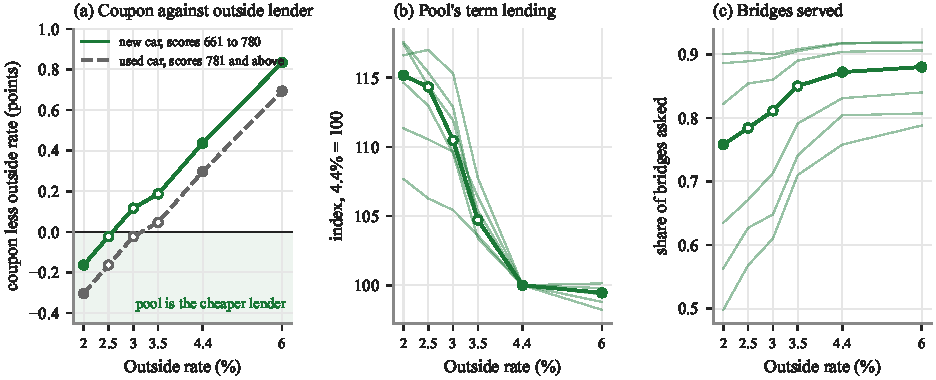
\includegraphics[width=\linewidth]{figures/fig_low_rates.pdf}
\caption{The edge at low outside rates, with no distress. (a) The pool's term coupon less the outside lender's rate
on the two kinds of vehicle loan of Table~\ref{tab:lending}; the pool lends such a loan where the difference is
not above zero. (b) The pool's term lending, each launch level set to 100 at an outside rate of 4.4\%. (c) Bridges
served. Thin lines are launch levels and the thick line their median. Hollow markers are the exploratory rate
cut.}
\label{fig:lowrates}
\end{figure}

\subsection{Stress}\label{sec:stress}

Table~\ref{tab:stress} and Figure~\ref{fig:stress} show where the result ends. Under distress the share of bridges
the pool serves in years 4 and 5 falls, and falls further the higher launch participation is. At 2 points and
an outside rate of 4.4\% a pool run, bridges served below 60\%, appears in at least one of the \NumSeeds{} seeds from \RunAdoption{}
launch participation upward; at an outside rate of 2\% runs begin at lower participation and lower distress
(Figure~\ref{fig:stress}). A run starts when a write-off takes owners' realised return below their alternative:
owners file to leave, the cash set aside for them cannot be lent, and long loans cannot be called. Bridges served
can fall below 60\% without owners leaving: with no distress they do in 1 of the \NumSeeds{} seeds at a launch of
60\% and in 6 at 80\%, where the pool is stretched (Table~\ref{tab:stress}).

Payments still fail less often under CPM on average: \FailCpmStressMean{} at 2 points of distress, against
\FailBanksStressMean{} under banks and cards and \FailDefiStressMean{} under best-case DeFi. That is
\FailCutBanksStress{} and \FailCutDefiStress{} lower, where with no distress it is \FailCutBanks{} and
\FailCutDefi{}. Across the whole grid,
by the share of payments that fail, CPM fails fewer than both alternatives in \CellsFewerFailures{} of \CellsAll{} cells. The six exceptions
all lie at an outside rate of 2\%, at launch participation of 45\% and above and distress of 1 point and above
(Figure~\ref{fig:failed}).

The gains above are earned over the whole run, which includes two years before the shock. Counting only
what is earned after it, in months 37 to 60, CPM's gain in money over banks and cards is positive in
\GainAfterBanksPositive{} of the \CellsAll{} cells, the lowest being \GainAfterBanksLow{} a person a year. Over
best-case DeFi it is positive in \GainAfterDefiPositive{}. The cells where it is negative, the lowest at
\GainAfterDefiLow{}, lie in the same corner: an outside rate of 2\%, launch participation of 45\% and above and
distress of 1.5 points and above, where owners run on the pool. There a household is still ahead over the sixty months
and is losing ground to best-case DeFi when the run ends. At 2 points the median cell earns
\GainAfterBanksMedianTwo{} a person a year over banks and cards after the shock and \GainAfterDefiMedianTwo{} over
best-case DeFi, against \GainAfterBanksMedianZero{} and \GainAfterDefiMedianZero{} over the same months with no
distress: \GainAfterBanksLowerTwo{} and \GainAfterDefiLowerTwo{} less.

The registered region narrows with distress: \RegionCellsHalf{} cells at half a point, \RegionCellsOne{} at 1
point, \RegionCellsOneHalf{} at 1.5 points and \RegionCellsTwo{} at 2 points (Table~\ref{tab:region}). At an
outside rate of 2\% no cell withstands half a point. At 4.4\% and 6\% launch levels of 20\% and 30\% withstand 2
points, launch levels of 5\%, 10\% and 45\% withstand 1.5 points, and launch levels of 60\% and 80\% withstand 1
point, or half a point at 6\% and a launch of 80\%. The claim withstands the most distress in the middle of the
launch range, and the two ends fail for different reasons. At launches of 5\% and 10\% the 2-point level fails on
clause (a): too few seeds read Persistent, though the pool still serves most of the bridges asked of it. At
launches of 45\% and above the level that fails does so on the dip in payments and on real cost, where the pool
serves about half the bridges asked of it.

\begin{figure}[htbp]\centering
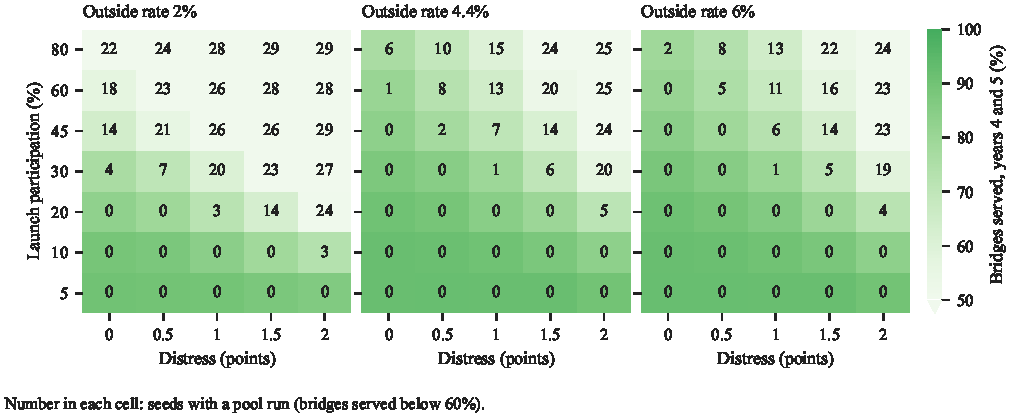
\includegraphics[width=\linewidth]{figures/fig_stress_boundary.pdf}
\caption{Bridges served under CPM in years 4 and 5, by launch participation and distress level, one panel per
outside rate. The number in each cell is the count of seeds, of \NumSeeds{}, with a pool run.}
\label{fig:stress}
\end{figure}

\begin{table}[htbp]\centering\footnotesize
\resizebox{\linewidth}{!}{% Written by scripts/paper_numbers.py from confirmation_quote.
\begin{tabular}{rrrrrrrr}
\toprule
Launch & Distress (pt) & Bridges served, years 4 and 5 & Seeds with a run (below 0.6) & Seeds below years 1 to 3 & Offers unused & Bridge write-offs (\$) & Term write-offs (\$) \\
\midrule
5\% & 0 & 0.918 & 0 of 30 & 4 of 30 & 79.4\% & \$0.4 & \$2.4 \\
5\% & 0.5 & 0.919 & 0 of 30 & 5 of 30 & 76.2\% & \$0.4 & \$3.0 \\
5\% & 1 & 0.915 & 0 of 30 & 10 of 30 & 71.7\% & \$0.4 & \$3.8 \\
5\% & 1.5 & 0.914 & 0 of 30 & 12 of 30 & 66.1\% & \$0.5 & \$4.4 \\
5\% & 2 & 0.896 & 0 of 30 & 13 of 30 & 57.4\% & \$0.9 & \$5.4 \\
10\% & 0 & 0.917 & 0 of 30 & 5 of 30 & 71.7\% & \$0.5 & \$3.3 \\
10\% & 0.5 & 0.914 & 0 of 30 & 7 of 30 & 67.2\% & \$0.6 & \$4.4 \\
10\% & 1 & 0.901 & 0 of 30 & 12 of 30 & 60.6\% & \$0.7 & \$5.5 \\
10\% & 1.5 & 0.877 & 0 of 30 & 18 of 30 & 53.1\% & \$0.8 & \$5.7 \\
10\% & 2 & 0.831 & 0 of 30 & 25 of 30 & 42.5\% & \$1.1 & \$6.4 \\
20\% & 0 & 0.904 & 0 of 30 & 13 of 30 & 61.0\% & \$0.6 & \$4.3 \\
20\% & 0.5 & 0.885 & 0 of 30 & 16 of 30 & 53.9\% & \$0.8 & \$5.3 \\
20\% & 1 & 0.843 & 0 of 30 & 23 of 30 & 45.2\% & \$0.9 & \$6.4 \\
20\% & 1.5 & 0.796 & 0 of 30 & 28 of 30 & 35.0\% & \$1.1 & \$7.0 \\
20\% & 2 & 0.708 & 5 of 30 & 29 of 30 & 23.2\% & \$1.4 & \$8.9 \\
30\% & 0 & 0.872 & 0 of 30 & 19 of 30 & 52.8\% & \$0.7 & \$5.3 \\
30\% & 0.5 & 0.845 & 0 of 30 & 20 of 30 & 44.5\% & \$1.0 & \$5.9 \\
30\% & 1 & 0.794 & 1 of 30 & 26 of 30 & 34.8\% & \$1.2 & \$7.7 \\
30\% & 1.5 & 0.698 & 6 of 30 & 30 of 30 & 23.2\% & \$1.4 & \$7.8 \\
30\% & 2 & 0.564 & 20 of 30 & 30 of 30 & 12.9\% & \$1.3 & \$9.6 \\
45\% & 0 & 0.831 & 0 of 30 & 24 of 30 & 45.7\% & \$1.0 & \$5.3 \\
45\% & 0.5 & 0.774 & 2 of 30 & 28 of 30 & 35.9\% & \$1.4 & \$6.4 \\
45\% & 1 & 0.702 & 7 of 30 & 28 of 30 & 24.0\% & \$1.5 & \$7.2 \\
45\% & 1.5 & 0.613 & 14 of 30 & 29 of 30 & 13.1\% & \$1.6 & \$8.0 \\
45\% & 2 & 0.453 & 24 of 30 & 29 of 30 & 4.5\% & \$1.7 & \$9.3 \\
60\% & 0 & 0.804 & 1 of 30 & 21 of 30 & 42.9\% & \$1.2 & \$6.2 \\
60\% & 0.5 & 0.725 & 8 of 30 & 23 of 30 & 31.9\% & \$1.3 & \$7.0 \\
60\% & 1 & 0.643 & 13 of 30 & 27 of 30 & 20.7\% & \$1.5 & \$7.8 \\
60\% & 1.5 & 0.523 & 20 of 30 & 28 of 30 & 11.7\% & \$1.8 & \$8.8 \\
60\% & 2 & 0.384 & 25 of 30 & 29 of 30 & 5.1\% & \$1.6 & \$11 \\
80\% & 0 & 0.758 & 6 of 30 & 20 of 30 & 37.5\% & \$1.3 & \$5.0 \\
80\% & 0.5 & 0.687 & 10 of 30 & 22 of 30 & 27.4\% & \$1.5 & \$6.6 \\
80\% & 1 & 0.597 & 15 of 30 & 24 of 30 & 16.6\% & \$1.5 & \$7.3 \\
80\% & 1.5 & 0.461 & 24 of 30 & 27 of 30 & 9.6\% & \$1.8 & \$8.8 \\
80\% & 2 & 0.329 & 25 of 30 & 29 of 30 & 4.4\% & \$1.8 & \$10 \\
\bottomrule
\end{tabular}
}
\caption{CPM under distress at an outside rate of 4.4\%: bridges served in years 4 and 5, the seeds with a pool run,
the seeds whose bridges served fall below their own level in years 1 to 3, the share of offers to the pool left
unused, and write-offs in dollars a person a year.}
\label{tab:stress}
\end{table}

\subsection{When savers judge the pool by its record}\label{sec:record}

The confirmation map was run again on the same seeds with one rule changed. Under the quote rule, the
decided one, a saver who reviews entry offers its money when the pool's published quote is at least the saver's
alternative. Under the record rule it does so when the pool's realised return over the last twelve months is.
The record rule is the pessimistic reading of the condition in Proposition~\ref{prop:capital}.
Table~\ref{tab:readings} sets the two rules side by side.

CPM stays ahead of both alternatives under either rule. Every gain over banks and cards and over best-case DeFi is
positive in \ReadSecondGainPositive{} of the \CellsAll{} cells of the grid. The median gain is
\ReadSecondGainBanks{} a person a year over banks and cards and \ReadSecondGainDefi{} over best-case DeFi,
\ReadSecondGainBanksLower{} and \ReadSecondGainDefiLower{} below the gains under the quote rule. CPM
fails \ReadSecondFailCpm{} of payments against \ReadSecondFailBanks{} under banks and cards. The real-cost clause
and the group clause pass in all \CellsNoDistress{} cells with no distress, as built and under the cash-advance
bound, and no falsifier fires.

The rule decides whether the pool sustains itself. Over years 4 and 5 pool capital stands at
\ReadSecondCapital{} of its target, against \ReadFirstCapital{} under the quote rule, and the pool serves
\ReadSecondServedCpm{} of the bridges asked of it, against \ReadFirstServedCpm{}. The pool is Persistent in \ReadSecondPersistentLow{} to
\ReadSecondPersistentHigh{} of the \NumSeeds{} seeds, depending on the cell, where clause (a) needs
\WilsonConfirm{}. That clause fails in all but \ReadSecondRegion{} cells, so under this reading the registered
claim holds in \ReadSecondRegion{} of the \CellsNoDistress{} cells with no distress and in none under distress.
The condition of Proposition~\ref{prop:capital} is the knife-edge of the design, and these numbers are its size.

Neither level of capital is a resting point. Table~\ref{tab:path} follows the pool year by year and Figure~\ref{fig:path} month by month. Its capital target rises
throughout the run under both rules, as the network grows and the term book fills: the longest loans run
sixty months, so the book is still filling when the run ends. Under the quote rule capital follows the
target to within one per cent for four years and stands at \PathFirstRatioFive{} of it in the fifth. Under the
record rule capital falls behind from the first year. It is \PathSecondRatioFour{} of the target in year 4
and \PathSecondRatioFive{} in year 5, and bridges served fall from \PathSecondServedFour{} to
\PathSecondServedFive{}. Capital still grows in dollars, from \PathSecondCapitalFour{} to \PathSecondCapitalFive{}
a person, but more slowly than what is asked of it. So sixty months do not show where the pool comes to
rest under this reading, only that it has not come to rest and is still losing ground when the run ends.

The record rule is also where demurrage does most. Without the charge the pool serves \ReadSecondServedPool{} of
bridges at a price of \ReadSecondPricePool{} and fails \ReadSecondFailPool{} of payments, close to the bank
arrangement. With the charge it serves \ReadSecondServedCpm{} at \ReadSecondPriceCpm{}. CPM's gain over the pool
without the charge is \ReadSecondGainOverPool{} a person a year under this reading, against
\ReadFirstGainOverPool{} under the quote rule. The two maps share their seeds and the bank arrangement is
the same in both, so they are one body of evidence read under two assumptions, not two confirmations.

\begin{table}[htbp]\centering\small
% Written by scripts/paper_numbers.py from confirmation_quote.
\begin{tabular}{lrr}
\toprule
 & Quote rule & Record rule \\
\midrule
Cells in the registered region, no distress & 19 & 2 \\
Seeds in which the pool persists & 26 to 30 & 6 to 23 \\
Pool capital over its target & 0.97 & 0.77 \\
\midrule
Bridges served, CPM & 0.84 & 0.52 \\
Bridges served, pool without the charge & 0.77 & 0.17 \\
Bridge price, CPM & 2.1\% & 2.4\% \\
Bridge price, pool without the charge & 6.7\% & 11.4\% \\
Payments that fail, banks and cards & 3.65\% & 3.65\% \\
Payments that fail, pool without the charge & 2.59\% & 3.35\% \\
Payments that fail, CPM & 2.51\% & 2.86\% \\
Gain over banks and cards & \$262 & \$217 \\
Gain over best-case DeFi & \$140 & \$90 \\
Gain over the pool without the charge & \$15 & \$61 \\
\midrule
Cells of the grid with every gain positive & 105 & 105 \\
Cells of the grid with fewer failed payments than both & 99 & 98 \\
\bottomrule
\end{tabular}

\caption{The confirmation map under the two entry rules, on the same \NumSeeds{} seeds: medians over
the \CellsNoDistress{} cells with no distress, and counts of cells. The second row is the range over those cells of
the number of seeds, of \NumSeeds{}, where the pool reads Persistent.}
\label{tab:readings}
\end{table}

\begin{table}[htbp]\centering\small
\resizebox{\linewidth}{!}{% Written by scripts/paper_numbers.py from confirmation_quote.
\begin{tabular}{lrrrrrrrr}
\toprule
 & \multicolumn{4}{c}{Quote rule} & \multicolumn{4}{c}{Record rule} \\
Year after launch & Capital over target & Capital, \$ & Target, \$ & Bridges served & Capital over target & Capital, \$ & Target, \$ & Bridges served \\
\midrule
1 & 1.01 & \$293 & \$292 & 0.87 & 0.97 & \$287 & \$298 & 0.81 \\
2 & 1.00 & \$614 & \$611 & 0.90 & 0.91 & \$563 & \$630 & 0.72 \\
3 & 1.00 & \$899 & \$895 & 0.90 & 0.91 & \$792 & \$884 & 0.70 \\
4 & 1.00 & \$1{,}284 & \$1{,}286 & 0.88 & 0.85 & \$1{,}040 & \$1{,}241 & 0.59 \\
5 & 0.96 & \$1{,}653 & \$1{,}728 & 0.80 & 0.75 & \$1{,}152 & \$1{,}564 & 0.43 \\
\bottomrule
\end{tabular}
}
\caption{The pool year by year after launch under the two entry rules, with no distress: for each
year the median over the \CellsNoDistress{} cells of the seed mean of the year's months. Capital and its target
are in dollars a person.}
\label{tab:path}
\end{table}

\begin{figure}[htbp]\centering
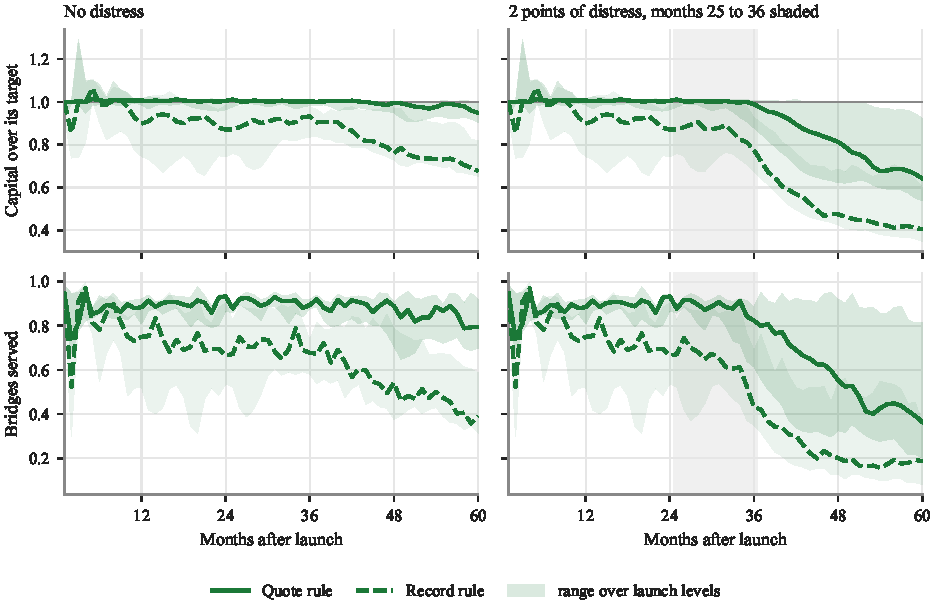
\includegraphics[width=\linewidth]{figures/fig_path.pdf}
\caption{Pool capital over its target (top) and bridges served (bottom), month by month after launch at an outside
rate of 4.4\%, under the quote rule and the record rule: the median over the seven launch levels of each cell's
seed mean, and their range. Left, no distress; right, 2 points of distress.}
\label{fig:path}
\end{figure}

\section{Robustness}\label{sec:robustness}

The checks here stand beside the confirmation map and outside the registered reading. Most ran
on the \NumSeedsDev{} development seeds and stand beside the development map on those seeds: the side checks,
the two bounds, the update scheme, the adoption rule with the network and the launch, and the chains of failure.
The exploratory side checks ran after the confirmation was read, on seeds kept for that purpose, and the size
check on its own seeds. Each subsection names its seeds.

\subsection{Side checks and bounds}

Eleven side checks rerun three launch levels (5\%, 20\% and 60\%, at an outside rate of 4.4\%), each with no
distress and at 2 points, six cells in all, on the development seeds with one setting changed. They are read beside the development map
on the same seeds. Halving or doubling the noise in the leaving rule, the low and the
high fixed cost, and pricing failures past the monthly fee cap at zero leave CPM's gains within a few per cent of
the development map's. Allowing five failure fees a month, not two, raises them. Cutting card lines in the
distress year raises failed payments in every arrangement and leaves CPM's gain unchanged. The record rule of
Section~\ref{sec:record}, here on the development seeds and three launch levels, gives the same picture: the pool serves
fewer bridges, and CPM's gains over both alternatives shrink but stay positive in every cell, with and without
distress (Table~\ref{tab:side}).

\begin{table}[htbp]\centering\small
\resizebox{\linewidth}{!}{% Written by scripts/paper_numbers.py from confirmation_quote.
\begin{tabular}{lrrrrrrrrr}
\toprule
 & \multicolumn{3}{c}{Gain over banks and cards} & \multicolumn{3}{c}{Gain over best-case DeFi} & \multicolumn{3}{c}{Bridges served at 2 points} \\
Launch participation & 5\% & 20\% & 60\% & 5\% & 20\% & 60\% & 5\% & 20\% & 60\% \\
\midrule
development map & \$119 & \$243 & \$465 & \$62 & \$124 & \$226 & 0.92 & 0.78 & 0.50 \\
\midrule
leaving noise halved & \$119 & \$244 & \$467 & \$61 & \$124 & \$227 & 0.93 & 0.81 & 0.52 \\
leaving noise doubled & \$119 & \$243 & \$460 & \$62 & \$125 & \$222 & 0.91 & 0.76 & 0.46 \\
fixed cost low & \$119 & \$244 & \$465 & \$62 & \$124 & \$226 & 0.92 & 0.77 & 0.47 \\
fixed cost high & \$119 & \$245 & \$465 & \$62 & \$125 & \$226 & 0.92 & 0.80 & 0.50 \\
entrants read the track record & \$116 & \$217 & \$396 & \$59 & \$98 & \$157 & 0.66 & 0.26 & 0.34 \\
entrants read it with noise & \$119 & \$236 & \$399 & \$61 & \$116 & \$160 & 0.81 & 0.47 & 0.32 \\
failures past the fee cap at zero & \$119 & \$244 & \$465 & \$62 & \$124 & \$226 & 0.92 & 0.78 & 0.50 \\
five failure fees a month & \$131 & \$265 & \$502 & \$76 & \$149 & \$268 & 0.89 & 0.74 & 0.46 \\
card lines cut in the distress year & \$119 & \$243 & \$465 & \$62 & \$124 & \$226 & 0.91 & 0.76 & 0.50 \\
half re-choose their buffer each month & \$118 & \$243 & \$459 & \$61 & \$124 & \$221 & 0.92 & 0.81 & 0.48 \\
15.3\% re-choose their buffer each month & \$117 & \$240 & \$449 & \$60 & \$120 & \$210 & 0.92 & 0.82 & 0.52 \\
\bottomrule
\end{tabular}
}
\caption{Side checks on three cells at an outside rate of 4.4\%, one setting changed in each, on the development
seeds: CPM's gain in money, in dollars a person a year with no distress, and bridges served in years 4 and 5 at 2
points of distress.}
\label{tab:side}
\end{table}

Two bounds rerun the whole development map on its seeds (Table~\ref{tab:bounds}). In the first the pool loses, and
prices, the published charge-off rate of each class of loan, where the model as built collects a written-off debt
later. The bridge price rises, as it must. CPM's gains are almost unchanged and every gain stays positive in every
cell. As many cells with no distress are stable (Persistent and passing the group clause on a majority of seeds,
the second view of Section~\ref{sec:measurement}) as on the development map. Fewer are stable under the
cash-advance bound as well, the table's last column.

The second is the outer bound on money paid to outside lenders. As built, the interest and fees households
pay to outside lenders and card issuers leave the household economy, so what a household saves by borrowing from
the pool counts as its gain. In the bound all that money returns to households in proportion to their
spending, as if they owned the lenders outright and lending cost nothing to supply. CPM's gain in money over
banks and cards falls by more than half but stays positive in every cell. Its gain in money over best-case DeFi
falls to zero. Its gain with completed purchases counted stays positive against both in every cell, and it fails
fewer payments than both in every cell. On a majority of seeds no cell is stable under this bound, because the
group clause is read in money against banks and cards.

The bound is exact about what the two kinds of gain are. Against best-case DeFi, CPM's gain in money is a
transfer: interest and fees households no longer pay to outside lenders. Its real gain is the payments that
no longer fail, delivered with the same real resources (Table~\ref{tab:gains}). How much of the transfer counts
as a gain to households depends on who owns the lenders. As built nobody in the model does, which leans toward
CPM; in the bound everybody does, which leans against it; households in fact own a small share. At the sourced
share, a tenth of lenders' income returning to households as the lenders' owners, the median gain in money is
\GainBanksShared{} over banks and cards and \GainDefiShared{} over best-case DeFi, read from the confirmation map as built with
no change in behaviour. On that reading the gain over best-case DeFi reaches zero only when a share of
\LenderShareZeroDefi{} of lenders' income returns to households.

\begin{table}[htbp]\centering\small
\resizebox{\linewidth}{!}{% Written by scripts/paper_numbers.py from confirmation_quote.
\begin{tabular}{lrrrrrrrrr}
\toprule
Map & Gain over banks & Gain over DeFi & Banks, purchases counted & DeFi, purchases counted & Every gain positive & Fewer failed payments & Bridge price & Stable as built & Stable both ways \\
\midrule
development map & \$296 & \$156 & \$611 & \$503 & 105 of 105 & 104 of 105 & 2.1\% & 14 of 21 & 11 of 21 \\
\midrule
loan losses at published rates & \$291 & \$151 & \$659 & \$499 & 105 of 105 & 105 of 105 & 5.5\% & 14 of 21 & 8 of 21 \\
lenders' interest returned & \$131 & $-$\$1.0 & \$413 & \$262 & 0 of 105 & 105 of 105 & 2.1\% & 0 of 21 & 0 of 21 \\
\bottomrule
\end{tabular}
}
\caption{The two bound maps beside the development map, each the whole grid on the same development seeds. Gains are medians over the
cells with no distress, in dollars a person a year, in money alone and with completed purchases at their price.
Counts of cells with every gain positive and with fewer failed payments are over the whole grid; the last two
columns count cells with no distress that are stable on a majority of seeds.}
\label{tab:bounds}
\end{table}

\subsection{The stress boundary in finer steps}

The grid's distress levels are half a point apart. On the \NumSeedsDev{} development seeds a finer cut between 1.5 and 2
points at three launch levels shows the shape of the boundary (Table~\ref{tab:boundary}). Bridges served fall
smoothly with distress at every launch level, with no cliff. On a majority of these seeds owners run on the
pool from \BoundaryFortyFive{} at a launch of 45\%, and at launches of 20\% and 30\% at no level up to 2 points.
On the \NumSeeds{} confirmation seeds runs are more frequent (Table~\ref{tab:stress}); the cut shows how bridges served
fall, not where the boundary lies. The nine runs of this cut with no distress repeat cells of the development map
and reproduce all \BoundaryRepeatValues{} of their stored values.

\begin{table}[htbp]\centering\small
\resizebox{\linewidth}{!}{% Written by scripts/paper_numbers.py from confirmation_quote.
\begin{tabular}{rrrrrrr}
\toprule
 & \multicolumn{2}{c}{Launch 20\%} & \multicolumn{2}{c}{Launch 30\%} & \multicolumn{2}{c}{Launch 45\%} \\
Distress (pt) & Bridges served & Seeds with a run & Bridges served & Seeds with a run & Bridges served & Seeds with a run \\
\midrule
1.5 & 0.852 & 0 of 3 & 0.767 & 0 of 3 & 0.721 & 0 of 3 \\
1.6 & 0.844 & 0 of 3 & 0.739 & 0 of 3 & 0.686 & 0 of 3 \\
1.7 & 0.833 & 0 of 3 & 0.725 & 0 of 3 & 0.619 & 1 of 3 \\
1.8 & 0.820 & 0 of 3 & 0.692 & 0 of 3 & 0.584 & 2 of 3 \\
1.9 & 0.805 & 0 of 3 & 0.670 & 0 of 3 & 0.548 & 3 of 3 \\
2.0 & 0.780 & 0 of 3 & 0.641 & 1 of 3 & 0.487 & 3 of 3 \\
\bottomrule
\end{tabular}
}
\caption{The stress boundary at an outside rate of 4.4\%: bridges served under CPM in years 4 and 5 (seed mean) and
the seeds where the pool is run, by distress level in steps of a tenth of a point and by launch participation.}
\label{tab:boundary}
\end{table}

\subsection{Exploratory side checks}

Four further checks ran after the confirmation map was read, each on \ExploreSeeds{} seeds of the exploratory
block and the six cells of the side checks above, beside a base run of the same cells on the same seeds
(Table~\ref{tab:explore}). They are exploratory, and three seeds cannot be read against the claim.

\emph{The fixed cost.} At its sourced level the pool's fixed cost is \SpiralCostSourced{} a person a year, since
every consumer unit carries it, so the threshold of Proposition~\ref{prop:threshold} is far from binding in
the maps. Table~\ref{tab:spiral} raises it. At ten times the sourced cost little moves. At a hundred times,
\SpiralCostHundred{} a person a year, the coupon carries the cost: the bridge price is above ten per cent a year at
every launch level, the more so the smaller the network, and CPM's gains stay positive. At a thousand times,
\SpiralCostThousand{} a person a year, the remaining lending cannot carry it. The bridge price runs from several
hundred to several thousand per cent, participation in years 4 and 5 falls well below the base's, and the gain over banks and cards is
negative at the two lower launch levels and positive only at a launch of 60\%. This is the threshold of
Proposition~\ref{prop:threshold} in simulation: the pool carries a fixed cost up to a bound set by its lending,
and higher adoption moves the bound.

\emph{The two price inputs.} With the issuer's custody cost raised from 0.24\% to 0.44\% a year, at which P yields
no more than best-case DeFi before the charge, and to 0.74\%, CPM's gain over best-case DeFi stays positive at
every launch level: at 0.74\% it is \ExploreCustodyDefiLow{} to \ExploreCustodyDefiHigh{} a person a year, against
\ExploreBaseDefiLow{} to \ExploreBaseDefiHigh{} in the base. The gain does not rest on the custody cost. With the
owners' spread at 0 or 0.5 point the gains move little, and bridges served under distress are lowest with no
spread.

\emph{The date of the shock.} With the distress year starting after month 12, not after month 24, CPM fails
\ExploreShockEarlyFailLow{} to \ExploreShockEarlyFailHigh{} of payments at 2 points against
\ExploreShockEarlyBanksHigh{} under banks and cards; starting at month 36 it fails \ExploreShockLateFailLow{} to
\ExploreShockLateFailHigh{} against \ExploreShockLateBanksHigh{}. CPM is ahead at both dates. The reading window
stays years 4 and 5, so levels at different dates are not comparable.

\emph{Low outside rates.} At outside rates of 0.5\% and 1\% (Table~\ref{tab:lowrates}) the charge falls to a few
hundredths of a per cent, CPM's gains over both alternatives stay positive, and with no distress it fails fewer
payments than banks and cards (not shown in the table). At 2 points of distress and a launch of 60\% it fails more, as it does at 2\% in
the registered map. The pattern of the lowest registered rate continues below it.

\begin{table}[htbp]\centering\small
\resizebox{\linewidth}{!}{% Written by scripts/paper_numbers.py from confirmation_quote.
\begin{tabular}{lrrrrrrrrr}
\toprule
 & \multicolumn{3}{c}{Gain over banks and cards} & \multicolumn{3}{c}{Gain over best-case DeFi} & \multicolumn{3}{c}{Bridges served at 2 points} \\
Launch participation & 5\% & 20\% & 60\% & 5\% & 20\% & 60\% & 5\% & 20\% & 60\% \\
\midrule
base & \$114 & \$245 & \$452 & \$60 & \$125 & \$217 & 0.89 & 0.67 & 0.43 \\
\midrule
fixed cost 10 times & \$110 & \$243 & \$445 & \$56 & \$123 & \$211 & 0.91 & 0.79 & 0.47 \\
fixed cost 100 times & \$68 & \$201 & \$417 & \$14 & \$81 & \$182 & 0.97 & 0.97 & 0.97 \\
fixed cost 1,000 times & $-$\$350 & $-$\$111 & \$96 & $-$\$404 & $-$\$230 & $-$\$139 & 1.00 & 1.00 & 0.99 \\
custody cost 0.44\% & \$111 & \$239 & \$437 & \$57 & \$120 & \$203 & 0.89 & 0.67 & 0.42 \\
custody cost 0.74\% & \$107 & \$231 & \$427 & \$53 & \$111 & \$192 & 0.89 & 0.66 & 0.41 \\
owners' spread 0 & \$113 & \$242 & \$439 & \$59 & \$122 & \$205 & 0.87 & 0.59 & 0.34 \\
owners' spread 0.5 point & \$114 & \$245 & \$454 & \$60 & \$125 & \$219 & 0.89 & 0.69 & 0.40 \\
shock from month 12 & \$114 & \$245 & \$452 & \$60 & \$125 & \$217 & 0.89 & 0.66 & 0.36 \\
shock from month 36 & \$114 & \$245 & \$452 & \$60 & \$125 & \$217 & 0.90 & 0.70 & 0.63 \\
\bottomrule
\end{tabular}
}
\caption{Exploratory side checks on \ExploreSeeds{} seeds, six cells at an outside rate of 4.4\%, one setting
changed in each: CPM's gain in money, in dollars a person a year with no distress, and bridges served in years 4
and 5 at 2 points of distress.}
\label{tab:explore}
\end{table}

\begin{table}[htbp]\centering\small
\resizebox{\linewidth}{!}{% Written by scripts/paper_numbers.py from confirmation_quote.
\begin{tabular}{lrrrrrrrrrr}
\toprule
 & & \multicolumn{3}{c}{Bridge price} & \multicolumn{3}{c}{Participation, years 4 and 5} & \multicolumn{3}{c}{Gain over banks and cards} \\
Fixed cost & \$ a person a year & 5\% & 20\% & 60\% & 5\% & 20\% & 60\% & 5\% & 20\% & 60\% \\
\midrule
sourced & \$0.18 & 2.1\% & 2.1\% & 2.1\% & 0.35 & 0.60 & 0.88 & \$114 & \$245 & \$452 \\
\midrule
fixed cost 10 times & \$1.79 & 2.7\% & 2.4\% & 2.3\% & 0.35 & 0.60 & 0.89 & \$110 & \$243 & \$445 \\
fixed cost 100 times & \$18 & 67.2\% & 23.1\% & 10.8\% & 0.31 & 0.60 & 0.89 & \$68 & \$201 & \$417 \\
fixed cost 1,000 times & \$179 & 3450.8\% & 1497.9\% & 650.2\% & 0.16 & 0.35 & 0.70 & $-$\$350 & $-$\$111 & \$96 \\
\bottomrule
\end{tabular}
}
\caption{The pool's fixed cost at its sourced level and at multiples of it, with no distress, by launch
participation: the price of a bridge, participation in years 4 and 5 and CPM's gain over banks and cards in
dollars a person a year. Exploratory, \ExploreSeeds{} seeds.}
\label{tab:spiral}
\end{table}

\begin{table}[htbp]\centering\small
\resizebox{\linewidth}{!}{% Written by scripts/paper_numbers.py from confirmation_quote.
\begin{tabular}{lrrrrrrrrrrr}
\toprule
 & & \multicolumn{3}{c}{Gain over banks and cards} & \multicolumn{3}{c}{Gain over best-case DeFi} & \multicolumn{3}{c}{Failed under CPM, 2 points} & \\
Outside rate & Demurrage & 5\% & 20\% & 60\% & 5\% & 20\% & 60\% & 5\% & 20\% & 60\% & Banks, 2 points \\
\midrule
0.5\% & 0.032\% & \$47 & \$105 & \$192 & \$47 & \$105 & \$188 & 4.82\% & 5.11\% & 6.70\% & 5.58\% \\
1.0\% & 0.046\% & \$58 & \$126 & \$215 & \$50 & \$104 & \$158 & 4.87\% & 5.48\% & 7.12\% & 5.63\% \\
\midrule
4.4\% & 0.139\% & \$114 & \$245 & \$452 & \$60 & \$125 & \$217 & 4.70\% & 4.52\% & 4.86\% & 5.89\% \\
\bottomrule
\end{tabular}
}
\caption{Outside rates below the grid's, beside the base at 4.4\%, by launch participation: the holding charge at
a launch of 20\%, CPM's gains in dollars a person a year with no distress, and payments that fail at 2 points of
distress under CPM and under banks and cards. Exploratory, \ExploreSeeds{} seeds.}
\label{tab:lowrates}
\end{table}

\subsection{The update scheme}

Three readings test whether the results depend on the update scheme of Section~\ref{sec:updating}.

A result made by everyone moving at once shows as a series alternating about its trend month to month. For
every monthly series of every run of the development map, the trend, a centred five-month mean, was removed and the share of the
remainder's variance at a period of two months computed (Table~\ref{tab:periodtwo}). White noise through the same
filter gives \PeriodTwoWhiteNoise{} and a flip-flop \PeriodTwoFlipFlop{}. Participation, pool capital, the charge,
the coupons, buffers, offers and exits sit at the noise level: their largest median share is
\PeriodTwoOthersMost{}. One series has a two-month rhythm, the failed share of people not in a job-loss spell, with
a median share of \PeriodTwoBanks{} under banks and cards and \PeriodTwoCpm{} under CPM. Its size is
\PeriodTwoAmplitude{} of the series' level, and its direction follows the seed: it is positive in
\PeriodTwoSignFirstSeed{} of the runs on the first development seed, \PeriodTwoSignSecondSeed{} on the second and
\PeriodTwoSignThirdSeed{} on the third. An artefact of people starting and re-choosing together would have one
direction in every seed. The 60-day billing cycle gives a direction fixed by the seed, since each seed's
population holds slightly more 60-day billers in one parity of months than the other. It is a feature of the
calendar, and pooled bridging smooths it.

The one decision everyone takes in the same month is the cash buffer. Letting only a random half of people
re-choose it each month, or a random 15.3\%, the model's review chance, lowers CPM's gains slightly, most at the
highest launch level under the slower schedule, and leaves bridges served unchanged (the last two rows of
Table~\ref{tab:side}). The results do not rest on buffers moving together.

The day's settlement is simultaneous, and by Proposition~\ref{prop:settlement} it can differ from payment one at a
time only through a closed loop of payers without money. Every run records the payments that rest on such loops:
they are at most \NettingShareMost{} of completed value in any run, and with payments under one cent set aside
no payer was in such a loop on any day of the runs of Table~\ref{tab:chains} (Section~\ref{sec:chains}).

\begin{table}[htbp]\centering\small
\resizebox{\linewidth}{!}{% Written by scripts/paper_numbers.py from confirmation_quote.
\begin{tabular}{lrrrrrr}
\toprule
Series & Median share & Largest share & Amplitude over level & Positive, seed 20261021 & Positive, seed 20261022 & Positive, seed 20261023 \\
\midrule
Banks and cards & 0.17 & 0.44 & 0.60\% & 100\% & 0\% & 100\% \\
Best-case DeFi & 0.13 & 0.42 & 0.59\% & 100\% & 0\% & 100\% \\
Pool without the holding charge & 0.03 & 0.19 & 0.83\% & 92\% & 9\% & 100\% \\
CPM & 0.03 & 0.27 & 0.91\% & 95\% & 11\% & 100\% \\
Indexed CPM & 0.03 & 0.25 & 0.94\% & 95\% & 9\% & 100\% \\
\midrule
Every other series (largest median; largest job) & 0.06 & 0.27 &  &  &  &  \\
White noise through the same filter (mean; 95th percentile) & 0.015 & 0.059 &  &  &  &  \\
A flip-flop with noise 0.3 of its size & 0.93 &  &  &  &  &  \\
\bottomrule
\end{tabular}
}
\caption{The share of each monthly series' variance about its trend that lies at a period of two months, over the
runs of the development map. The upper rows are the failed share of people not in a job-loss spell, by arrangement,
with the size of the alternation against the series' level and the share of runs on each seed where its sign is
positive.}
\label{tab:periodtwo}
\end{table}

\subsection{The adoption rule, the network and the launch}

The base joins people by a simple contagion, draws sellers uniformly and scatters the launch. Table~\ref{tab:robust}
and Figure~\ref{fig:robustpaths} replace each of the three in turn, at an outside rate of 4.4\% with no distress,
on the development seeds.

\emph{Thresholds.} Under the threshold rule a person imitates only once the share of its trading partners in the
network reaches its own threshold, which it keeps for the run. The base rule is the case of a threshold drawn
afresh, uniformly, every month. Keeping the threshold sorts people: those with low thresholds join first, those
still outside hold the higher ones, and adoption falls behind. With uniform thresholds kept, participation from a
20\% launch runs below the base's by up to \RuleCheckGapMean{}, and the well-mixed path that follows the share
outside threshold by threshold reproduces the shortfall (Figure~\ref{fig:robustpaths}).

With the thresholds measured for a paid online service \cite{karsaicascades}, adoption is faster than under the
base rule: from a 5\% launch participation reaches \RobustMeasuredPartFive{} at month 60 against
\RobustBasePartFive{}, since about a sixth of people have a threshold below 5\%. With one common threshold
\cite{watts} the outcome turns on its height (Figure~\ref{fig:thresholdmap}). At 0.1 every launch level tips. At
0.3 launches of 5\% and 10\% do not tip within the run, but a launch of 20\% does: from 5\% participation reaches
\RobustThresholdThirtyPartFive{} by month 60, which is what innovation alone gives. At 0.2 the well-mixed hand case says a 5\% launch should not tip within five years, but it
does, reaching \RobustThresholdTwentyPartFive{}. A person meets the share among its own partners of the month,
which differs from person to person and counts each partner by how often the two deal, so some people are over
their threshold while the population is under it. A critical mass exists under a common threshold, but the network
a person sees blurs it. The rule fixed in advance for a critical mass, a rise of at least 0.05 over the
launch share by month 60, is met from the lowest launch level at every threshold, because innovation alone clears
it. It does not separate tipping from innovation; the comparison with the innovation path above does.

In every threshold run CPM's gain over banks and cards and over best-case DeFi survives in all seven launch cells,
positive on the seed mean and in at least two of three seeds. Where adoption stalls the gain per person is smaller,
since fewer people are in the network.

\emph{The ring.} On a ring where everyone buys only from its 32 nearest neighbours, the base rule with a
scattered launch gives the base's participation and gains almost to the dollar (Table~\ref{tab:robust}). Locality
of trade changes nothing by itself, because a scattered launch puts members in every neighbourhood. Launching in
one neighbourhood slows adoption under either rule: from a 5\% launch participation reaches
\RobustRingNeighbourhoodPartFive{} at month 60 against \RobustRingPartFive{} scattered under the base rule, and
\RobustRingThresholdNeighbourhoodPartFive{} against \RobustRingThresholdPartFive{} under a common threshold of 0.2.
A neighbourhood's members trade mostly with one another, so their example reaches few people outside and the
network grows at its edge. The theory of complex contagion favours a clustered start \cite{centolamacy},
but it does not help here; the reason is in the scattered runs above. With dozens of trading partners a month,
enough people cross a threshold of 0.2 from a scattered launch that it tips without clustering. When 35\% of
purchases are local, the share of card transactions made within a short walk of home \cite{farrell}, the
neighbourhood launch loses most of its handicap (\RobustRingLocalThresholdNeighbourhoodPartFive{} from 5\%).

\emph{Hub sellers.} With hub sellers, whose number of buyers has the tail measured on a community currency
\cite{mattsson,goh}, receipts are concentrated and payments fail more often in every arrangement, under banks and
cards as under CPM. CPM still fails fewer, and participation follows the base's path. Launching with the largest
sellers first speeds adoption from a small launch, \RobustHubsLargestPartFive{} at month 60 from 5\% against
\RobustHubsPartFive{}, since many people buy from a large seller.

In all fifteen variants CPM's gain over banks and cards and over best-case DeFi survives in each of the seven
launch cells. The adoption rule, the network and the launch change how fast the network fills, and with it the size
of the gain per person at a given date. They do not change its sign.

Two variants were also run under 2 points of distress, over the seven launch levels on the development
seeds: the ring with a scattered launch, and hub sellers, both under the base rule. On the ring CPM fails
\RobustStressRingFailCpm{} of payments, against \RobustStressRingFailBanks{} under banks and cards and
\RobustStressRingFailDefi{} under best-case DeFi. With hub sellers it fails \RobustStressHubsFailCpm{}, against
\RobustStressHubsFailBanks{} and \RobustStressHubsFailDefi{}. The base at the same cells reads
\RobustStressBaseFailCpm{}, \RobustStressBaseFailBanks{} and \RobustStressBaseFailDefi{}. In each of the three
worlds CPM fails fewer payments than both alternatives in all \RobustStressRingCells{} cells, and its gain in money
over both is positive in all. The pool is stretched alike: at a launch of 80\% it serves
\RobustStressRingServedHigh{} of the bridges asked of it on the ring and \RobustStressHubsServedHigh{} with hub
sellers, against \RobustStressBaseServedHigh{} in the base. On these seeds the comparison under distress is the
same on the ring and with hub sellers as on the uniform network. The other variants were not run under distress.

\begin{table}[htbp]\centering\small
\resizebox{\linewidth}{!}{% Written by scripts/paper_numbers.py from confirmation_quote.
\begin{tabular}{llrrrrrrrrrrrrrr}
\toprule
 & & \multicolumn{3}{c}{Participation at month 60} & \multicolumn{2}{c}{Gain over banks} & \multicolumn{2}{c}{Gain over DeFi} & \multicolumn{2}{c}{Cells where it survives} & \multicolumn{2}{c}{Failed payments} & & & \\
Sellers & Joining and launch & from 5\% & from 20\% & from 60\% & Median & Range & Median & Range & Banks & DeFi & CPM & Banks & Bridge price & Demurrage & Critical mass \\
\midrule
Uniform & linear joining (the base) & 0.45 & 0.69 & 0.92 & \$311 & \$119 to \$518 & \$156 & \$62 to \$233 & 7 of 7 & 7 of 7 & 2.03\% & 3.61\% & 2.10\% & 0.140\% &  \\
 & measured thresholds & 0.78 & 0.86 & 0.94 & \$382 & \$246 to \$523 & \$184 & \$123 to \$234 & 7 of 7 & 7 of 7 & 1.88\% & 3.61\% & 2.05\% & 0.145\% &  \\
 & common threshold 0.1 & 0.84 & 0.90 & 0.95 & \$398 & \$275 to \$524 & \$188 & \$133 to \$234 & 7 of 7 & 7 of 7 & 1.83\% & 3.61\% & 2.05\% & 0.144\% & 5\% \\
 & common threshold 0.2 & 0.54 & 0.89 & 0.95 & \$398 & \$96 to \$524 & \$189 & \$55 to \$234 & 7 of 7 & 7 of 7 & 1.83\% & 3.61\% & 2.08\% & 0.141\% & 5\% \\
 & common threshold 0.3 & 0.18 & 0.80 & 0.95 & \$385 & \$61 to \$524 & \$187 & \$31 to \$234 & 7 of 7 & 7 of 7 & 1.85\% & 3.61\% & 2.10\% & 0.140\% & 5\% \\
\midrule
Ring & local share 1, linear joining & 0.44 & 0.69 & 0.92 & \$312 & \$117 to \$530 & \$159 & \$61 to \$245 & 7 of 7 & 7 of 7 & 2.03\% & 3.72\% & 2.09\% & 0.149\% &  \\
 & local share 1, linear, one neighbourhood & 0.35 & 0.48 & 0.77 & \$245 & \$99 to \$501 & \$122 & \$50 to \$237 & 7 of 7 & 7 of 7 & 2.55\% & 3.72\% & 2.08\% & 0.145\% &  \\
 & local share 1, threshold 0.2 & 0.58 & 0.88 & 0.95 & \$394 & \$127 to \$535 & \$189 & \$69 to \$247 & 7 of 7 & 7 of 7 & 1.85\% & 3.72\% & 2.10\% & 0.153\% & 5\% \\
 & local share 1, threshold 0.2, one neighbourhood & 0.39 & 0.54 & 0.84 & \$243 & \$90 to \$503 & \$123 & \$48 to \$237 & 7 of 7 & 7 of 7 & 2.55\% & 3.72\% & 2.09\% & 0.141\% & 5\% \\
 & local share 0.35, linear joining & 0.44 & 0.69 & 0.92 & \$310 & \$116 to \$512 & \$157 & \$59 to \$228 & 7 of 7 & 7 of 7 & 2.07\% & 3.65\% & 2.06\% & 0.137\% &  \\
 & local share 0.35, threshold 0.2, one neighbourhood & 0.50 & 0.86 & 0.94 & \$379 & \$93 to \$514 & \$174 & \$53 to \$229 & 7 of 7 & 7 of 7 & 2.09\% & 3.65\% & 2.08\% & 0.132\% & 5\% \\
\midrule
Hubs & linear joining & 0.45 & 0.69 & 0.92 & \$314 & \$121 to \$533 & \$170 & \$66 to \$258 & 7 of 7 & 7 of 7 & 3.31\% & 5.09\% & 2.20\% & 0.211\% &  \\
 & linear joining, largest sellers first & 0.58 & 0.77 & 0.92 & \$359 & \$208 to \$534 & \$143 & \$85 to \$245 & 7 of 7 & 7 of 7 & 3.57\% & 5.09\% & 2.20\% & 0.175\% &  \\
 & measured thresholds & 0.78 & 0.85 & 0.93 & \$381 & \$249 to \$530 & \$191 & \$128 to \$250 & 7 of 7 & 7 of 7 & 3.12\% & 5.09\% & 2.19\% & 0.204\% &  \\
 & measured thresholds, largest sellers first & 0.82 & 0.86 & 0.93 & \$394 & \$313 to \$539 & \$158 & \$136 to \$248 & 7 of 7 & 7 of 7 & 3.41\% & 5.09\% & 2.17\% & 0.184\% &  \\
\bottomrule
\end{tabular}
}
\caption{The adoption rule, the sellers' network and the launch placement, each replaced in turn: seven launch
levels at an outside rate of 4.4\% with no distress, development seeds. Participation is the seed mean at month 60.
Gains are CPM's, in money, in dollars a person a year: the median over the seven cells and their range. A gain
survives in a cell when it is positive on the seed mean and in at least two of three seeds.}
\label{tab:robust}
\end{table}

\begin{figure}[htbp]\centering
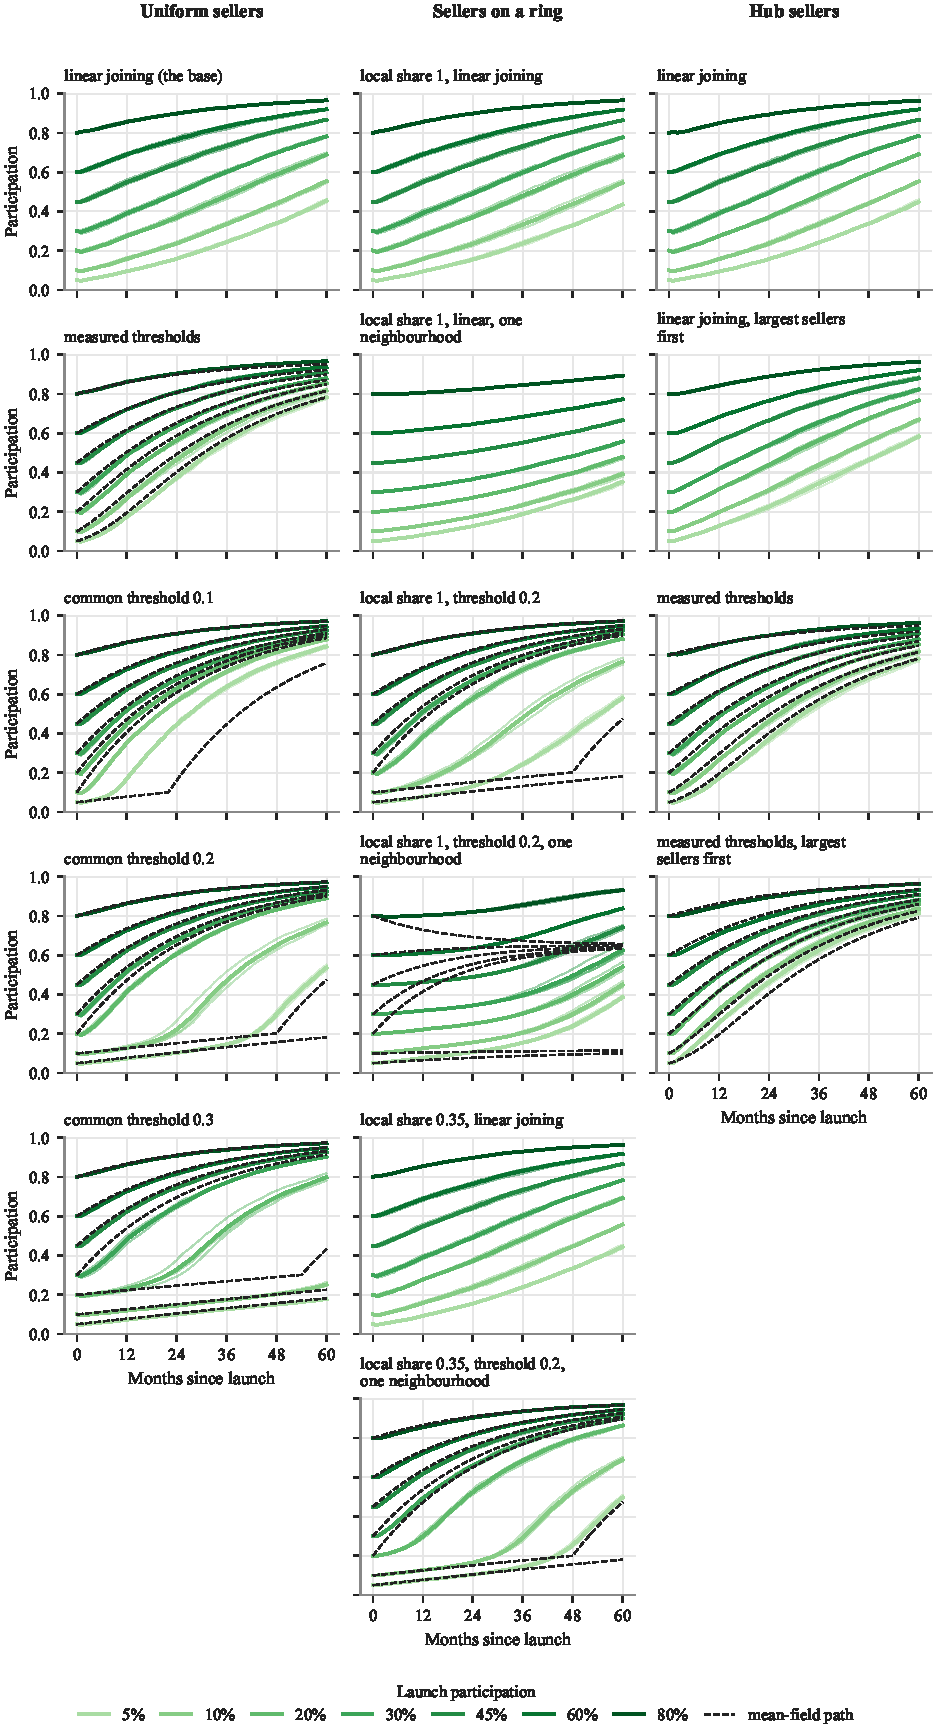
\includegraphics[width=\linewidth,height=0.86\textheight,keepaspectratio]{figures/fig_robust_paths.pdf}
\caption{Participation under CPM month by month in every variant, from the seven launch levels: the seed mean thick
and each seed thin. Dashed lines are the well-mixed path with each person's threshold kept, one leaving rate
fitted.}
\label{fig:robustpaths}
\end{figure}

\begin{figure}[htbp]\centering
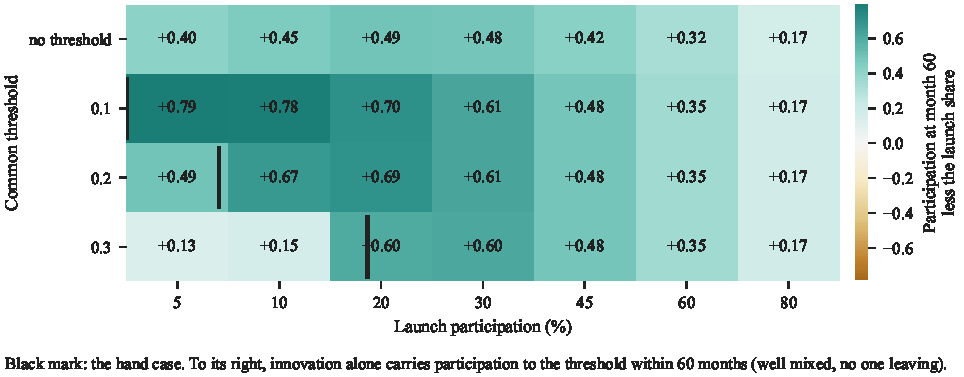
\includegraphics[width=\linewidth]{figures/fig_threshold_map.pdf}
\caption{Participation at month 60 less the launch share, by launch share and common threshold, uniform sellers.
The mark in each row is the hand case: to its right, innovation alone carries a well-mixed population to the
threshold within 60 months.}
\label{fig:thresholdmap}
\end{figure}

\subsection{Chains of failure}\label{sec:chains}

A failed payment is missing income for its payee, so failure can pass from payer to payee. Two readings measure how
far it does.

Within a day each payer's failure is split into the part it would fail even if paid in full that day and the part
due to short receipts, the fundamental and contagious defaults of \cite{elsinger}
(Table~\ref{tab:chains}). The second part is small: \KnockOnBanks{} of failed value under banks and cards and
\KnockOnCpm{} under CPM with no distress, \KnockOnBanksStress{} and \KnockOnCpmStress{} at 2 points. Under CPM it
is lower by \KnockOnGap{} of failed value with no distress (\KnockOnGapRange{} over cells and seeds); at 2 points
the range, \KnockOnGapStressRange{}, includes runs where it is higher. The pool changes who bears it. Under banks
and cards a knock-on failure touches a few payers on most days and never as many as 32. With a pool it touches many
borrowers at once on some days: 32 or more on \ManyKnockOnCpm{} of days under CPM and \ManyKnockOnPool{} in the
pool without the charge, and \ManyKnockOnCpmStress{} and \ManyKnockOnPoolStress{} at 2 points. When receipts fall
short the pool's cash is rationed pro rata, so one payer's shortfall is spread thinly over everyone who borrows that
day. More payers are touched and less value fails.

Across days no such split exists, since a failure today changes every later day. What can be read is how far a
shock spreads. A run at a distress level differs from the same seed's run with no distress only through the extra
layoffs, which can be drawn again from the seed, so the extra failed payments divide between the people an
extra layoff hit and everyone else (Table~\ref{tab:spread}, read on the development map, whose runs store each
person's failed payments). Between \SpreadWideLow{} and \SpreadWideHigh{} of the
excess over the three years from the shock falls on people not laid off, when everything a hit person
fails from its first hit on counts as its own, and \SpreadNarrowLow{} to \SpreadNarrowHigh{} when only what it
fails in a month it is hit does. The shares are alike in every arrangement and mix three channels: income
missing along the payment network, the wages of extra layoffs leaving the household economy, and the shift in
everyone's spending. They measure the spread of distress to people not laid off, not the length of a chain.

In the distress year the excess is lower under CPM than under banks and cards in \SpreadLowerYearHalf{},
\SpreadLowerYearOne{}, \SpreadLowerYearOneHalf{} and \SpreadLowerYearTwo{} of \SpreadCells{} cells at 0.5, 1, 1.5
and 2 points. Over the three years it is lower in \SpreadLowerHalf{}, \SpreadLowerOne{}, \SpreadLowerOneHalf{} and
\SpreadLowerTwo{}. At 2 points the median difference over the three years is \SpreadGapTwo{} failed shares a person
a year, against CPM: where the pool is run, those who relied on it lose more of what they had than those who
never had it. The level of failed payments is still lower under CPM (Table~\ref{tab:arrangements}); the excess is what a
shock adds to each arrangement's own level.

\begin{table}[htbp]\centering\small
\resizebox{\linewidth}{!}{% Written by scripts/paper_numbers.py from confirmation_quote.
\begin{tabular}{llrrrrrrrrrr}
\toprule
Distress & Arrangement & Knock-on share (median) & Knock-on share (range) & Payers a day (median) & Payers a day (range) & Days with 32 or more (median) & Days with 32 or more (range) & Netting share (median) & Netting share (range) & Netting days (median) & Netting days (range) \\
\midrule
None & Banks and cards & 0.57\% & 0.57\% & 2.4 & 2.4 & 0.0\% & 0.0\% & 0.000\% & 0.000\% & 0.0 & 0.0 \\
 & Best-case DeFi & 0.55\% & 0.53\% to 0.56\% & 2.3 & 2.2 to 2.4 & 0.0\% & 0.0\% & 0.000\% & 0.000\% & 0.0 & 0.0 \\
 & Pool without the holding charge & 0.44\% & 0.44\% to 0.52\% & 8.7 & 4.4 to 19.7 & 10.5\% & 4.5\% to 18.8\% & 0.000\% & 0.000\% & 0.0 & 0.0 \\
 & CPM & 0.41\% & 0.41\% to 0.51\% & 5.4 & 3.2 to 10.7 & 5.7\% & 2.6\% to 10.0\% & 0.000\% & 0.000\% & 0.0 & 0.0 \\
 & Indexed CPM & 0.42\% & 0.41\% to 0.51\% & 5.3 & 3.1 to 10.5 & 5.7\% & 2.5\% to 9.9\% & 0.000\% & 0.000\% & 0.0 & 0.0 \\
\midrule
2 points & Banks and cards & 0.84\% & 0.84\% & 3.8 & 3.8 & 0.0\% & 0.0\% & 0.000\% & 0.000\% & 0.0 & 0.0 \\
 & Best-case DeFi & 0.81\% & 0.76\% to 0.82\% & 3.7 & 3.5 to 3.8 & 0.0\% & 0.0\% & 0.000\% & 0.000\% & 0.0 & 0.0 \\
 & Pool without the holding charge & 0.69\% & 0.68\% to 0.78\% & 18.9 & 7.3 to 40.4 & 17.8\% & 7.2\% to 28.7\% & 0.000\% & 0.000\% & 0.0 & 0.0 \\
 & CPM & 0.69\% & 0.65\% to 0.76\% & 15.6 & 5.2 to 34.1 & 13.2\% & 3.7\% to 22.5\% & 0.000\% & 0.000\% & 0.0 & 0.0 \\
 & Indexed CPM & 0.69\% & 0.65\% to 0.79\% & 15.3 & 5.2 to 36.5 & 13.1\% & 3.8\% to 24.3\% & 0.000\% & 0.000\% & 0.0 & 0.0 \\
\bottomrule
\end{tabular}
}
\caption{Failure passed on within a day, on six cells (an outside rate of 4.4\%; launch participation of 5\%, 20\%
and 60\%): the share of failed value that fails only because receipts were short, the payers with such a failure a
day, the share of days when 32 or more payers had one, and the payments that rest on a closed loop of payers
without money. Medians and ranges over the three launch levels of the seed means.}
\label{tab:chains}
\end{table}

\begin{table}[htbp]\centering\small
\resizebox{\linewidth}{!}{% Written by scripts/paper_numbers.py from confirmation_quote.
\begin{tabular}{llrrrrrrr}
\toprule
Distress & Arrangement & Excess (median) & Excess (range) & Not hit, wide & Not hit, narrow & Distress year (median) & Distress year (range) & Not hit, distress year \\
\midrule
0.5 pt & Banks and cards & 0.783 & 0.764 to 0.786 & 0.92 & 0.95 & 0.306 & 0.302 to 0.307 & 0.75 \\
 & Best-case DeFi & 0.754 & 0.702 to 0.774 & 0.92 & 0.94 & 0.305 & 0.296 to 0.314 & 0.73 \\
 & Pool without the holding charge & 0.643 & 0.523 to 1.014 & 0.91 & 0.94 & 0.253 & 0.215 to 0.313 & 0.72 \\
 & CPM & 0.641 & 0.473 to 1.001 & 0.91 & 0.94 & 0.239 & 0.218 to 0.335 & 0.72 \\
\midrule
1 pt & Banks and cards & 1.645 & 1.595 to 1.664 & 0.89 & 0.95 & 0.621 & 0.613 to 0.625 & 0.72 \\
 & Best-case DeFi & 1.579 & 1.459 to 1.613 & 0.89 & 0.95 & 0.626 & 0.614 to 0.655 & 0.70 \\
 & Pool without the holding charge & 1.444 & 1.254 to 2.094 & 0.90 & 0.95 & 0.527 & 0.448 to 0.655 & 0.70 \\
 & CPM & 1.373 & 1.242 to 2.339 & 0.89 & 0.95 & 0.519 & 0.439 to 0.673 & 0.71 \\
\midrule
1.5 pt & Banks and cards & 2.590 & 2.512 to 2.631 & 0.85 & 0.95 & 0.952 & 0.941 to 0.957 & 0.69 \\
 & Best-case DeFi & 2.492 & 2.306 to 2.558 & 0.85 & 0.94 & 0.958 & 0.940 to 0.998 & 0.68 \\
 & Pool without the holding charge & 2.440 & 2.071 to 3.524 & 0.86 & 0.95 & 0.848 & 0.702 to 1.016 & 0.67 \\
 & CPM & 2.286 & 2.075 to 3.735 & 0.86 & 0.94 & 0.841 & 0.647 to 0.997 & 0.67 \\
\midrule
2 pt & Banks and cards & 3.726 & 3.602 to 3.803 & 0.82 & 0.94 & 1.252 & 1.236 to 1.263 & 0.68 \\
 & Best-case DeFi & 3.561 & 3.248 to 3.685 & 0.82 & 0.94 & 1.259 & 1.239 to 1.317 & 0.67 \\
 & Pool without the holding charge & 3.948 & 3.046 to 5.019 & 0.84 & 0.95 & 1.117 & 0.952 to 1.460 & 0.66 \\
 & CPM & 3.919 & 2.999 to 5.223 & 0.84 & 0.95 & 1.084 & 0.861 to 1.413 & 0.66 \\
\bottomrule
\end{tabular}
}
\caption{The extra failed payments at a distress level over the same seed's run with no distress, in failed shares
of bills and wages a person a year, over the three years from the shock and in the distress year: medians and
ranges over the 21 cells of a level of the seed means, with the share that falls on people no extra layoff hit.}
\label{tab:spread}
\end{table}

\subsection{Population size}

Figure~\ref{fig:size} shows the size check beside the choice of \NumPeople{} people (Section~\ref{sec:measurement}): eight seeds kept for nothing
else, at five population sizes. CPM's gains over banks and cards and over best-case DeFi do not move with size.
The gain over the pool without the charge grows with size, so the present population understates what the charge
adds. The count of seeds with a pool run at 2 points rises with size, then levels off: small populations hide
the stress boundary, and it is not an artefact of size.

\begin{figure}[htbp]\centering
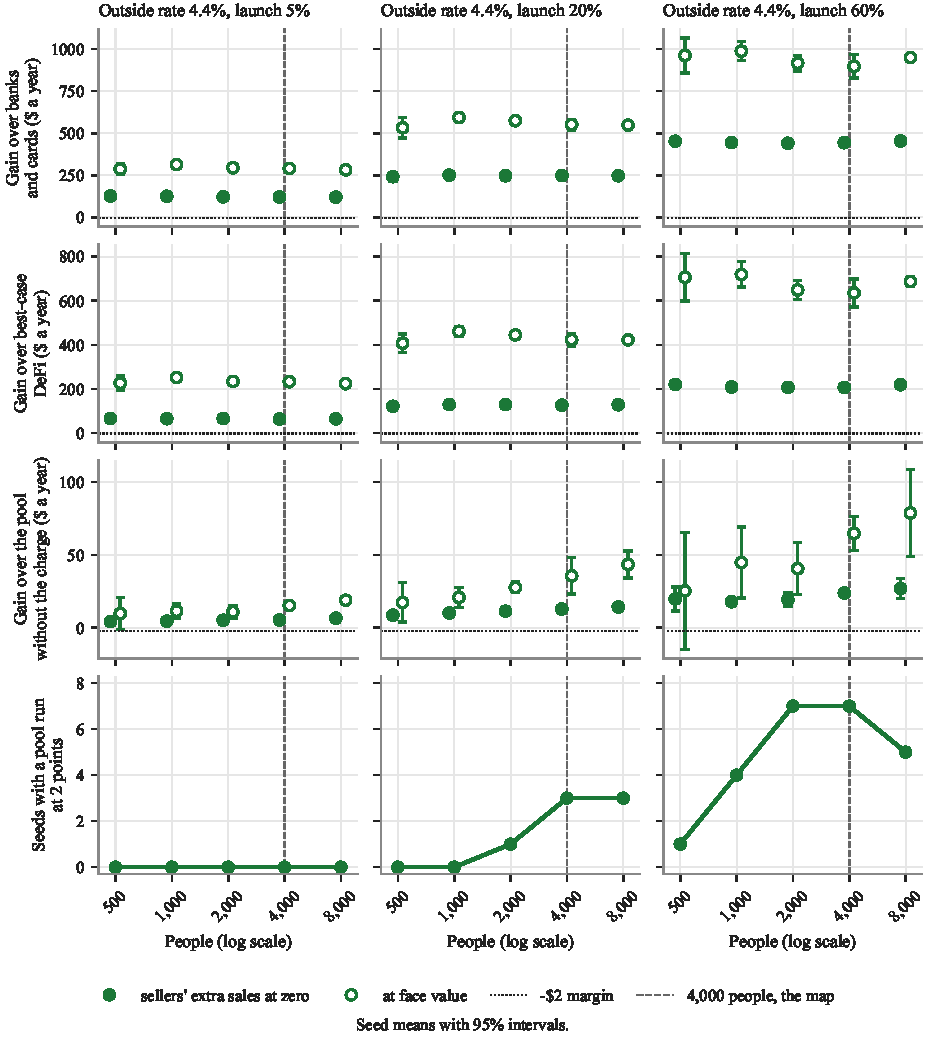
\includegraphics[width=0.92\linewidth]{figures/fig_size_check.pdf}
\caption{The population size check, three cells at an outside rate of 4.4\%: CPM's gain over banks and cards, over
best-case DeFi and over the pool without the charge, and the number of seeds, of eight, with a pool run at 2
points of distress, against population size.}
\label{fig:size}
\end{figure}


\section{Limits}\label{sec:limits}

This section collects what bounds the result, with the direction each limit leans where known. It
has four groups: the boundaries of the result, the modelling choices that lean towards or against CPM, the
method, and the inputs and the standing of the evidence.

\subsection{Boundaries of the result}

\emph{The stress boundary.} Under 2 points of distress owners can run on the pool. At 2 points they leave after a
write-off takes their realised return below their alternative, pool capital falls short, and bridges served drop:
on the first development check at $a_{0} = 0.6$ this happened in two of three seeds, with bridges served of 0.29 and
0.30 in years 4 and 5 against 0.90 in the third. The repeated size check counts the seeds with such a run, bridges
served below 0.6 in years 4 and 5, out of eight at each population of 500, 1,000, 2,000, 4,000 and 8,000: none at any
size at $a_{0} = 0.05$; 0, 0, 1, 3 and 3 at $a_{0} = 0.2$; and 1, 4, 7, 7 and 5 at $a_{0} = 0.6$. Where runs occur the counts rise with
population and then level off, and one falls back at the largest size. The run does not go away as the population
grows, so it is a boundary of the design at every size, reached from 20\% launch
participation upward at 2,000 people and more, and populations of 500 to 1,000 hide it. Its cause is long loans funded by capital on two months' notice. Term
lending stays in the model, with the bridge and term parts of the pool's book, income and losses reported
apart. Changing the cash set aside for exits or ranking bridges first after seeing the result would favour the
pool, so neither is done. The limit leans against CPM where it binds. On the size check's three cells at 4,000
people CPM still fails fewer payments than the bank arrangement in all eight seeds at 2 points, and its mean gain
over the bank arrangement and over best-case DeFi is positive in every seed. On the confirmation map the mean gain
is positive in every cell at every level of distress, and CPM fails fewer payments in \CellsFewerFailures{} of the
\CellsAll{} cells (Section~\ref{sec:results}). Figure~\ref{fig:stress} and Table~\ref{tab:stress} show the cells and seeds
with a pool run at each level of distress.

\emph{How a run unfolds.} An owner reviews its holding with a chance of 15.3\% a month, a rate decided for users and
with no source for investors, reads only its own realised return, and does not react to other owners leaving. The
exit notice is fixed at two months. A run where owners leave because others are leaving, the first-mover
advantage of the literature on fund runs, is therefore absent, and the stress boundary is a lower
bound on run risk. This leans toward CPM. Neither the review rate nor the notice is varied.

\emph{Capital and the published quote.} Pool capital holds at its target under the quote rule, because entrants
act on the published quote, which with no fee margin equals their alternative. Under the record rule, when they
read the pool's realised twelve-month return instead, capital sat below 95\% of its target in 29 to 51\% of months on the development checks, at 1,000 and
4,000 people, while the gain over best-case DeFi stayed positive. The quote rule leans toward CPM. The record
rule is run over the confirmation map as the pessimistic one, with its own region. A third rule, each saver
reading the record with the leaving rule's noise, is a side check on three cells. The record rule is one
pessimistic rule, not a proven worst case: savers who trusted the pool less than its own record would do
worse, and on one of the side check's nine numbers the noisy reading serves fewer bridges than it. The two maps
share their seeds and the bank arrangement, so they are one body of evidence read under two
assumptions, not two confirmations.

\emph{The shock, the low rates and the price inputs.} The registered maps hit the pool with one shock, in months
25 to 36, at outside rates of 2\% and above, with an owners' spread of 0.25 point and a custody cost of 0.24\%.
The exploratory side checks of Section~\ref{sec:robustness} move each of these on three seeds and six cells: they
change the sizes; the gains stay positive, and under 2 points of distress the low rates behave as the lowest registered
rate does. A shock in the first months after launch, a rate that moves within a run,
and a rate rise on a book of fixed coupons are not studied.

\subsection{Choices that lean one way}

\emph{Cash advances in the bank arrangement.} Card holders reach the card for bills and wages only through cash
advances. By inference from the model's weights about four fifths of those advances pay wages the holder owes
as an employer, which consumer cash
advances do not pay in practice. On the development check holders' cash advances ran about 15 times the United
States level (\$1,777 a person a year against \$112 to \$118 a consumer unit) and their fees about 31 times (\$163
against \$5.33). The fees avoided were 11 to 27\% of CPM's wealth gain over the bank arrangement and 38 to 50\% of its
gain over best-case DeFi, so the excess leans toward CPM. The card contract is left as built, every gain is
reported with the cash-advance fees and interest saved taken out, and a cell counts in the region only if it passes
both ways.

\emph{The bank arrangement's alternatives.} A payer short under banks and cards can draw on savings, a card
cash advance, a revolved card balance or earned-wage access. Payday loans, buy now pay later and loans from family
are not in the model, and a failed payment is charged the \$27 fee without the bank paying the item, as an
overdraft would. Each gives the bank arrangement fewer ways to cover a shortfall than households have,
which leans toward CPM.

\emph{Best-case DeFi is generous to DeFi.} It keeps the full reserve-funded savings yield, converts to and from bank
money at no fee where $P$ pays about 0.2\%, is accepted by every seller, and bears none of its own
operational or legal risks. Its over-collateralised loan is in the arrangement as it is: a payer who is short has
already used its own money and same-day savings, so nothing is left to lock and the loan covers none of the
shortfall. Each leans against CPM. On the registered clause every group is ahead of best-case DeFi; the
money-only number is the premium paid by people never short, and it decides no verdict.

\emph{No growth.} Total spending is fixed, and no production, growth or wider-economy effect is modelled: a firm that
borrows earns no more afterwards, and completed trade creates no income. This leans against CPM, and is why
completed trade is reported beside the headline as a bracket from zero to face value, not inside it. In the
other direction, a failed bill is erased, not paid later, so completed-trade dollars are an upper bound.

\emph{Owners' return.} Owners' return against their alternative has a loss tail that shrinks with population. One
loan is a share of the pool that falls as one over the number of people: at 1,000 people a single business loan reached 15\% of the
pool and one default drove a shortfall, while at 4,000 owners earned their alternative in every year on an earlier
development check. A loan of \$25,000 to \$100,000 is still 0.7\% of the pool at 8,000. The model also has no permanent default,
since a written-off debt stays owed and is collected later, which keeps bridge losses near zero and leans toward
CPM on the bridge price. The loan-loss bound prices the published charge-off rates instead. Owners' return against
their alternative is reported with its interval and read by no verdict; a separate falsifier fires only if owners'
return is shown below DeFi's savings rate. On the confirmation map owners' return less their alternative has a
median within \OwnersMedianWorst{} of a percentage point of zero at every outside rate, and one seed-cell in ten falls
short by \OwnersTenthLeast{} to \OwnersTenthWorst{} of a point or more (Table~\ref{tab:owners}).

\subsection{Method}

\emph{A paired transient.} Each run lasts 60 months after launch and every gain is measured during a transition:
participation is still growing in most cells when the run ends, so the comparison is of two paths from the same
start over the same five years, not of two steady states. The lowest launch level is 5\%, so neither a launch from
an empty network nor a long-run state is shown. The direction of this limit is not known. The mean wealth gain is
also read at 36 and 48 months (Table~\ref{tab:gains}), and Figure~\ref{fig:participation} shows participation still
rising at month 60 from every launch level.

\emph{Settlement within a day.} The model's day has no earlier and later. Payments due on a day are settled
together, money received can be paid on within the day, and where more than one outcome fits the
day's rules the one with the most payments completed is taken (Proposition~\ref{prop:settlement}). This is the same
in every arrangement and leans toward completion in each. The payments that rest on the choice of outcome are at
most \NettingShareMost{} of completed value in any run, so the comparison between arrangements does not turn on
it. The daily clock removes failure through timing within a day, from every arrangement alike.

\emph{A day the settlement cannot resolve.} When the pool's cash is short its requests are served pro rata and the
day's map need not be monotone (Section~\ref{sec:updating}). The model resolves two states that repeat when a
request qualifies in one and fails the repayment check in the other. A day when the iteration still does not
come to rest has no further rule: the model stops the run and does not guess. This happened in no run of the two
confirmation maps or the side checks. It happened in \CutSeedsAside{} of the \CutSeedsTried{} seeds of
the rate cut, once each, at outside rates of 3\% and 3.5\%; each such seed is set aside whole and named in the
cut's record. The cut is therefore read on the seeds where every run completed, and what those four seeds would
have shown is not known.

\emph{Chains of failure.} Failure passed on within a day is measured exactly. Failure passed on across days is not:
the spread of a shock to people not laid off mixes the payment network with the money that extra layoffs'
wages take out of the household economy and with the shift in everyone's spending. A count of chains across days
would need a record of receipts lost by payee and a run where those wages stay inside the economy.

\emph{What demurrage adds on its own.} CPM against the pool without the charge, on the same people and draws, is
what the holding charge adds. This edge has not settled with population size: it grows at every doubling from 500 to
8,000 people. With completed purchases at their price, as the size check reads it, between 4,000 and 8,000
it moves from \$15.4 to \$19.0 a person a year at $a_{0} = 0.05$, from
\$35.6 to \$43.5 at $a_{0} = 0.2$ (inside its interval) and from \$64.8 to \$78.8 at $a_{0} = 0.6$. At 4,000 people the paper therefore understates what the
charge adds, which leans against CPM.

\emph{The adoption rule and the network.} The base joins people by a simple contagion among trading partners drawn
uniformly, with a scattered launch. Section~\ref{sec:robustness} replaces each on the development seeds, and the sign
of CPM's gain survives every replacement while the speed of adoption does not. Thresholds for a payment money have
not been measured: the measured ones are those of one paid online service, and a common threshold is a design, not
an estimate. Under a common threshold of 0.3 a launch of 10\% or less does not tip within five years, and the gain
per person is then the smaller gain of a network that stays small. The hub world's tail is that of the number of
trading partners in one community currency, whose source could not estimate the tail of amounts; a heavier tail, a
network grown from payment data and one that changes as people join are not modelled. Wage links are uniform in
every world.

\subsection{Inputs and evidence}

\emph{Inputs and their sources.} The model's inputs are United States figures, each listed with its value and
source in Appendix~\ref{app:parameters}, as in the agent-based models used in central banks. The question is
whether CPM moves money better in that economy; no output forecasts a quantity of the United States economy. Some
inputs are proxies or have no primary source: the 1.7\% merchant card fee, found only in trade
press, which scales the saving against the bank arrangement and leaves the comparison with best-case DeFi unchanged;
the issuer's cost of 0.24\% of $P$, a money-market fund expense ratio; the 43\% debt cap; and the loan terms.
Mortgages are left out. No unemployment insurance is modelled, which overstates the losses of workers hit by the
stress and leans against the pool, since benefits would be receipts a bridge lends against.

\emph{Inputs set by declaration.} The parameter table marks each input as sourced or declared. Of those
declared or resting on a proxy, the leaving noise, the fixed cost, the failure-fee cap, the buffer review share, the
custody cost, the owners' spread and the date of the shock have a sensitivity run. The shape and median of initial wealth, the
spending elasticity, the wage share, the number of purchases a month, the twelve-month windows, the debt-to-income
limit, the exit notice and the review rate have none. The direction in which each would move the result is not
known.

\emph{Where the robustness checks sit.} The checks of Section~\ref{sec:robustness} other than the two bound maps and
the spread of distress are run at the central outside rate of 4.4\%: the side checks, the finer cut of the stress
boundary and the adoption, network and launch variants on development seeds, the exploratory side checks on three
side seeds, and the size check on its own eight. The two bound maps cover all three rates. Nothing here shows that the variants
leave the result unchanged at 2\% or 6\%.

\emph{What registered means.} The claim, its tests and the seed count were fixed in the dated record of decisions
and the analysis plan shipped with the code, before any confirmation seed was run. They were not deposited with a
public registry, so their dates rest on that record. The plan lists its departures from earlier registered
text, and the two additions made after the first confirmation map was read, the rate cut and the exploratory side
checks, are labelled exploratory there and here.

\emph{Development and confirmation.} The headline results and the registered claim are read on the confirmation
map, \SeedsConfirm{} seeds never run before the freeze and read once after it. The loan-loss bound, the
interest-returned bound, the side checks, the finer cut of the stress boundary, the robustness sets, the
update-scheme reading and the spread of distress are read on the three development seeds, on which the model was
built and its rules decided, and the size check on eight seeds of its own. Each is labelled so, and none is
confirmed.


% ====================================================================================================================
\section{Conclusion}
\label{sec:conclusion}
Circulation-Priced Money asks the holders of a payment money to pay a small
demurrage, and uses it for one purpose: to pay the capital cost of liquidity
that a pool they own keeps ready. The resulting contract
has no free rate or share, and its prices can be checked line by line against
the code that runs it. On \NumSeeds{} confirmation seeds, read once and as
registered, the arrangement does what it was designed to do. The registered
claim holds in \RegionCellsZero{} of the \CellsNoDistress{} cells with no
distress. With no distress the share of payments that fail is
\FailCutBanks{} below that of banks and cards, and at the median cell
households pay \OutsideCutBanks{} less to the intermediaries outside the
household economy. Fewer payments fail
than under banks and cards or under best-case
decentralised finance in \CellsFewerFailures{} of the \CellsAll{} cells of
the grid, and every cell shows a gain over both over the sixty months, with and
without distress. Real
resources are saved against banks and matched to within two dollars a person
a year against decentralised finance. Owners earn their alternative at the
median, and the
demurrage stays below a fifth of one per cent a year.

Demurrage, the holding charge, is the smallest number in the arrangement and has one
defined job. It costs a holder a few dollars a year. For that the price of a
bridge to whoever is short falls by half or more, the pool keeps cash
standing by against the peak of demand and lends more, balances revolved on
cards fall, fewer payments fail, and household wealth is
\GainPerChargeDollar{} dollars higher for each dollar collected than under the
same pool without it. It does this as insurance does, by moving a
cost from the person in trouble to everyone who holds the money. It does not
do it by making money move faster: the speed of circulation differs by about
one per cent with and without the charge. The pool supplies the credit; demurrage
makes that credit cheap and keeps it available.

The result has three boundaries. At the lowest outside rate the claim misses
in two cells with no distress and holds in none under distress: there is less
reserve return to pass on, and the pool, then the cheaper lender on long
vehicle loans, has less cash left for bridging. Under a wage loss of the
size of 2009 the pool, which funds long loans with capital on two months'
notice, can suffer a run at high launch participation; in
\GainAfterDefiBehind{} cells of
the grid, all at the lowest outside rate, what a household earns after the
shock then falls short of best-case decentralised finance. And pool capital
stays near its target, within one per cent for four years and at
\PathFirstRatioFive{} of it in the fifth, only under the quote rule, while savers enter on the
published quote; under the record rule, when they enter on the pool's realised
return, it has not come to rest by the end of the run. None
of these is
removed here; each is measured and reported. The registered claim was read
once, on \SeedsConfirm{} seeds held back for the purpose, and that reading is
the test of the arrangement. The side checks, bounds and robustness sets on
development seeds are reported beside it and are not confirmed.

The study is deliberately narrow. It asks what demurrage does for payments
and short credit among households, with spending, production and prices
given. The economy-wide questions, among them the effect on saving
and investment, on bank funding and on monetary policy, are left to
work that can now start from a contract with no free parameter and a
measured account of where it holds.

\section*{Code and data}
The model, the experiment, the registered analysis plan, the test suite and
the stored results of every map and check reported here are in the repository
that accompanies this draft, \url{https://github.com/cpm-research/circulation-priced-money}. Every results table and every figure drawn from
data is written from the stored results by \texttt{scripts/rebuild\_paper.py},
which runs no simulation, and \texttt{paper/numbers\_report.txt} traces each
number to the stored field it was read from. \texttt{paper/README.md} lists,
for each table and figure, the function that writes it and the results it
reads. Each equation of the contract is recomputed from a run's own records by
a test (Appendix~\ref{app:code}), each calibrated value is listed with its
source and checked against the code (Appendix~\ref{app:parameters}), and each
stored file is listed with its SHA-256 hash. The monthly records of the three
largest maps, about a gigabyte, are attached to the repository's release
\texttt{draft-2026-11}.

\appendix
\section{The ledger and conservation}
\label{app:ledger}
Money in the model moves only between named accounts, and every flow has a
payer and a receiver. Three identities follow. Each is checked on the
simulation's own records by a test named in Table~\ref{tab:ledger}.

\paragraph{Accounts.}
A person holds bank money, \(P\), outside savings and pool shares at net asset
value, and owes its payables, card balances and loans. The pool holds
cash and loans; the only claims on it are its owners' shares and any
unpaid operating bill. The issuer holds the reserve behind all
\(P\) and nothing else. Outside lenders, card networks, the conversion
provider, the pool's operating provider and validators sit outside the
household economy. What households pay them leaves it, what they pay
households enters it, and both are recorded as outside flows.

\paragraph{Wealth.}
Let \(\Delta V_m\) be the change in the sum of all people's net financial
wealth in month \(m\), \(X_m\) the net flow from outside, \(U_m\) the
revaluation of pool loans, recoveries less write-downs, and \(J_m\) the change
in the real value of nominal stocks through inflation. Then
\begin{equation}
\Delta V_m \;=\; X_m+U_m+J_m
\label{eq:wealth}
\end{equation}
in every month and every arrangement, to \(10^{-12}\) of a month's mean
spending. The holding charge does not appear in \eqref{eq:wealth}. It is
withheld from wallet holders' yield and credited to the pool, whose shares
households own, so it moves wealth between people and never across the
boundary of the household economy.

\paragraph{Backing.}
The reserve changes only when \(P\) is issued or redeemed, one for one. It
therefore equals the \(P\) outstanding, in wallets and in the pool's
cash, after every step. The backing of \(P\) is checked, not assumed.

\paragraph{Funded credit.}
The pool pays out only cash it holds. A loan moves existing \(P\) from the
pool to the borrower, an exit is paid from pool cash or a new
subscription, and a cost the pool cannot pay is its creditor's loss. No step
creates money. Shares are issued and redeemed at net asset value.

\begin{table}[htbp]\centering\small
\begin{tabularx}{\linewidth}{@{}lL@{}}
\toprule
Identity & Test \\
\midrule
Wealth, equation \eqref{eq:wealth} & \path{test_wage_dated_budget_keeps_the_accounting_identity_in_every_arm} \\
The charge stays among households & \path{test_eq11_charges_stay_in_the_household_economy} \\
Backing & \path{test_reserves_follow_every_issue_and_redemption},
\path{test_backing_holds_in_every_setup_and_is_untracked_without_an_issuer} \\
Funded credit & \path{test_insolvent_closure_creates_no_money} \\
\bottomrule
\end{tabularx}
\caption{The identities of the ledger and the tests that check them, in
\texttt{tests/test\_economy\_abm.py} and \texttt{tests/test\_contract\_equations.py}.}
\label{tab:ledger}
\end{table}

\section{Equations and the code that computes them}
\label{app:code}
Table~\ref{tab:code} ties each equation of Section~\ref{sec:contract} to the
simulation function that computes it and to a test that recomputes it.
Each test runs the simulation itself, records what every step read and wrote,
and checks the equation in every month from the inputs it names. The
runs cover CPM, the pool without the charge, indexed CPM, CPM under the
loan-loss bound, and a run where the cap on the charge binds; a bridge and
a term loan are forced past due so losses and recoveries occur. ``Exact''
means equality bit for bit. ``\(10^{-12}\)'' means agreement to that relative
tolerance, used where the test adds the same terms in another order.

{\small
\begin{longtable}{@{}p{0.20\textwidth}p{0.24\textwidth}p{0.36\textwidth}p{0.12\textwidth}@{}}
\caption{Each equation, the function that computes it and the test that
recomputes it. The tests are in \texttt{tests/test\_contract\_equations.py}.}
\label{tab:code}\\
\toprule
Equation & Function & Test & Agreement \\
\midrule
\endfirsthead
\toprule
Equation & Function & Test & Agreement \\
\midrule
\endhead
\bottomrule
\endfoot
Coupon \eqref{eq:coupon}, fixed-cost rate \eqref{eq:fixed}
 & \path{_cycle_terms}, \path{_fixed_rate}
 & \path{test_eq01_coupon_is_alternative_plus_operating_plus_fixed_plus_loss}
 & \(10^{-12}\) \\
Peak \eqref{eq:peak}, standby \eqref{eq:standby}, capital cost \eqref{eq:cost}
 & \path{_kept_ready}, \path{_cycle_terms}
 & \path{test_eq02_capital_cost_of_liquidity_kept_ready}
 & \(10^{-12}\) \\
Holding charge \eqref{eq:charge}
 & \path{_cycle_terms}, \path{_reserve_return}
 & \path{test_eq03_holding_charge_is_capital_cost_over_wallet_capped_at_p}
 & \(10^{-12}\); exact at the cap \\
Coverage \eqref{eq:coverage}, bridge price \eqref{eq:bridgeprice}
 & \path{_cycle_terms}; sealed in \path{_settle}
 & \path{test_eq04_coverage_and_the_bridge_price}
 & price exact; coverage \(10^{-12}\) \\
Yield on \(P\) \eqref{eq:yield}
 & \path{_cycle_terms}
 & \path{test_eq05_p_yield}
 & exact \\
The charge's share \(\theta\) (Proposition~\ref{prop:theta})
 & \path{_accrue}, \path{_close}
 & \path{test_eq06_theta_is_the_charges_share_of_bridging_finance}
 & exact; weighted form \(10^{-12}\) \\
Target \eqref{eq:target}, quote \eqref{eq:quote}
 & \path{_limit}, \path{_quote}, \path{paper_return}
 & \path{test_eq07_capital_target_and_quote}
 & quote exact; target \(10^{-12}\) \\
Entry and exit \eqref{eq:exit}
 & \path{_dealing}, \path{_reviews_entry}, \path{_exits}, \path{_leave_chance}
 & \path{test_eq08_entry_pro_rata_to_the_target_and_exit_by_the_logistic}
 & who files and is paid exact; amounts \(10^{-12}\) \\
Learned loss \eqref{eq:loss}
 & \path{_loss_rates}, \path{_write_off}
 & \path{test_eq09_learned_loss}
 & \(10^{-12}\) \\
No charge in the pool without it
 & \path{_cycle_terms}, \path{_limit}
 & \path{test_eq10_no_charge_in_u}
 & exact \\
The charge stays among households (Proposition~\ref{prop:incidence})
 & \path{_reserve_return}
 & \path{test_eq11_charges_stay_in_the_household_economy}
 & exact \\
\end{longtable}
}

Two properties of the code go beyond the equations as printed. Coverage
computed as \(c\,\cyc W/K\) with \(c=K/\cyc W\) can fall one unit in the last
binary place below one, so the bridge price can differ from \(o+f+\ell_b\) by
about \(10^{-19}\) a month. And in the month after launch the launch plan,
which has no term lending, enters the two-month average of the term lending
need.

\section{Parameters and sources}\label{app:parameters}

Table~\ref{tab:parameters} lists every calibrated value and every setting that affects the results, in the units a
reader would quote; the code holds money in months of mean spending (\$6,440) and rates a month. The same table in
machine form, with each value in the code's own units and the code's own name, is \texttt{docs/PARAMETERS.csv}, and a
test fails if any value in it differs from the code. ``Declared'' marks a modelling choice, not a sourced fact. The
sources were checked against the publishers' own pages and documents in November 2026; where a published figure
differs from the value used, the Source column says so.

{\small
\setlength{\tabcolsep}{4pt}
\begin{longtable}{@{}p{0.17\textwidth}p{0.15\textwidth}p{0.08\textwidth}p{0.28\textwidth}p{0.24\textwidth}@{}}
\caption{Parameters, values and sources.}\label{tab:parameters}\\
\toprule
Symbol or name & Value & Unit & Meaning & Source \\
\midrule
\endfirsthead
\toprule
Symbol or name & Value & Unit & Meaning & Source \\
\midrule
\endhead
\bottomrule
\endfoot
\multicolumn{5}{@{}l}{\textit{Rates and costs}}\\
$\rho = r_{\mathrm{out}}$ & 2, 4.4, 6 & \% a year & reserve rate, the outside rate (a control) & three-month bill, declared grid \\
$o$ & 2 & \% a year & pool operating cost on carried principal & Philippon (2015), unit cost of US financial intermediation, applied to the pool \\
$\phi$ & 0.18 (0.10, 0.50) & \$ a person a year & pool fixed cost, central (low, high) & Aave (central), Compound (low), Sky (high) paid service providers, 2025, over 134.556m consumer units \\
$a - \rho$ & 0.25 & points a year & owners' spread in their alternative and in the coupon's capital part & declared \\
$c_I$ & 0.24 & \% a year & issuer's custody cost on all P; $p = \rho - c_I$ & ICI (2026), money market fund expense ratio, 2025, a proxy \\
merchant card fee & 1.7 & \% & paid by the seller on each card payment & CMSPI (2025), average acceptance cost over all payment types, 2022 \\
card rewards & 0.75 & \% & paid to the cardholder on card purchases & CFPB card market report (2025); Fed Payments Study (2024) \\
conversion fee & 0.05\% + \$0.22 & per conversion & dollars to P and back, the cents scaled to a \$142 payment & 12 CFR 235.3(b), 235.4(a); payment size declared \\
USDC conversion & 0 & \% & dollars to USDC and back & Coinbase Exchange fee table, June 2026 \\
gas & \$0.00169 & per transfer & one transfer for P, two for USDC & growthepie, Base, October 2026 \\
bill anchor & 4.05 (4.135) & \% a year & bill rate on a discount basis (credited monthly) & FRED TB3MS, October 2026 \\
USDC yield spread & 0.441 & points a year & bill less the Sky Savings Rate (3.60\%, 3.80\% APY) & sUSDS \texttt{ssr()} on Ethereum, October 2026 \\
deposit rate & 0.38 (floor 0.06) & \% a year & savings deposits at the anchor & FDIC national savings rate (FRED SNDR), October 2026; floor declared \\
pass-through & 0.08 / 1 / 0.75 / 0.63 / 1 & share & of $r_{\mathrm{out}}$ to deposit, card, vehicle, personal and business rates & FRED, 2022 to 2024; Fed G.19 against TB3MS, February 2022 to February 2024 \\
checking yield & 0.07 & \% a year & on bank money & FDIC national interest-checking rate, November 2026 \\
overdraft rate & 22 & \% a year & on rounding overdrafts & Fed G.19, credit card plans, Q3 2026 (21.19\% all accounts, 22.36\% accounts assessed interest) \\
DFA mix & table & \$ millions & deposits and money market shares by wealth group (bottom 50, 50--90, 90--99, top 1\%) & Fed Distributional Financial Accounts, 2026 Q2 \\
real cost, card credit & 3.4 & \% a year & of balances & Agarwal et al.\ (2015) \\
real cost, term credit & 2.5 & \% a year & of balances & FDIC Quarterly Banking Profile, Q4 2025 \\
real cost, failure & \$2 & per item & a failed payment, or a pool bridge that replaced one & CFPB overdraft rule, December 2024 \\
real cost, card rail & \$0.069; 0.11\%; 0.09\% & per payment; of value & processing and fraud prevention; fraud; network & Fed Regulation II data 2023; Nilson Report 2023; Visa 2025 \\
real cost, holding & 0.24 & \% a year & of money and savings balances & ICI (2026), money market fund expense ratio, 2025 \\
real cost, earned-wage advance & \$2 & per use & & declared \\
\midrule
\multicolumn{5}{@{}l}{\textit{Households and income}}\\
unit of money & \$6,440 & per month & mean consumer-unit spending & BLS, Consumer Expenditures in 2023 (2024) \\
Pareto shape & 1.5 & & initial wealth, by quantile band means & declared \\
median wealth & 0.6 & months of own spending & before survey cushions & declared \\
survey cushions & \$0, 100, 500, 2,000, 5,000 & at ranks 0, 0.18, 0.30, 0.50, 0.62 & liquid savings caps by rank & Federal Reserve Board (2026), SHED 2025, Table 26, largest emergency expense covered from savings \\
spending elasticity & 0.5 (floor 0.02) & & to relative net worth (floor of mean) & declared \\
wage share & 58.3 & \% of spending & one wage contract to one other person & declared \\
service purchases & 32 & a month & each to a random seller & declared \\
housing share & 32.9 & \% & of total expenditures, applied to service purchases, not card-eligible & BLS, Consumer Expenditures in 2023 (2024) \\
billing cycles & 1, 7, 15, 30, 60 & days & shares 20.9, 15.7, 36.6, 16.4, 10.4\% & BLS CES, length of pay period, February 2023, for wages; business split declared \\
pay periods & 7, 14, 15, 30 & days & shares 27.0, 43.0, 19.8, 10.3 (normalised) & BLS CES, length of pay period, February 2023, shares of establishments; day counts declared \\
buffer grid & 0 to 3 & months of own spending & 0, 0.1, 0.25, 0.5, 0.75, 1, 1.5, 2, 3 & declared \\
failure fee & \$27 & per failed bill or wage & at most one a day and two a month & Bankrate via Checkbook; monthly cap declared \\
request rates & 0.347/60, 0.185/24, 0.37/12 & a month & vehicle, personal, business & SCF 2022 (Federal Reserve Board, 2023), Table 4, vehicle and other instalment loans; business declared, near the Fed SBCS share applying for financing (37\% in 2023 and 2024) \\
terms & 60, 24, 11 & months & vehicle, personal, business & Fed G.19 (new car 60-month, personal 24-month); business declared \\
loan sizes & \$43,582 new, \$27,528 used (43.3\% new); \$7,000; 0.158 of a year's spending & for a mean spender, scaled by own spending & vehicle, personal, business & Experian (2026), Q4 2025, new and used; 43.3\% new declared (42.2\% reported, including leases); personal declared (TransUnion, Q2 2025: \$8,524 average); business declared, geometric midpoints of Fed SBCS 2019 bands \\
vehicle APR & 16.11 to 4.41 new; 21.62 to 6.29 used & \% a year & by five score tiers & Experian, State of the Automotive Finance Market, Q2 2026, VantageScore 4.0 tiers \\
personal APR & 17.97 to 10.82 & \% a year & at scores 620 to 740 & Experian (Curinos), September 2026, 36 months; August and November 2026 tables 0.2 to 0.6 point higher \\
business APR & 7.4 & \% a year & business loans & NFIB, Small Business Economic Trends, June 2026, short-maturity loans \\
debt-to-income limit & 43 & \% & household instalment credit & declared; the General QM limit of 12 CFR 1026.43(e)(2)(vi) until replaced in 2021 \\
earned-wage access & 7.43; 2.45; 50 & \% & holders (an upper bound); fee; share of unpaid wages & CFPB (2024); NCLC (2020) \\
inflation & 2 & \% a year & every arrangement & Federal Reserve target \\
\midrule
\multicolumn{5}{@{}l}{\textit{Cards}}\\
income brackets & 12.9, 15.6, 26.7, 44.8 & \% & households under \$25k, \$25--50k, \$50--100k, over \$100k & Census, CPS ASEC 2026, HINC-06 \\
card ownership & 46, 71, 88, 97 & \% & by income bracket & Federal Reserve Board (2026), SHED 2025, Table 40 \\
FICO bands & 14.7, 14.9, 20.1, 27.5, 22.8 & \% & below 580, 580--669, 670--739, 740--799, 800 and above & Experian, FICO Score distribution, September 2025 \\
score and income & 0.291 & rank correlation & Gaussian link 0.3036 & FEDS Notes, 13 August 2018, Table 1 \\
purchase APR & 28.49, 28.20, 22.99 & \% a year & scores to 619, 620--719, 720 and above & CFPB (2024), large issuers' median, January to June 2023 \\
credit line & 5,696; 8,121; 12,524; 22,068; 29,335; 41,654 & \$ & deep subprime to superprime & CFPB, Consumer Credit Card Market, 2025, Fig.~89 \\
start at 90--100\% & 68.41, 46.88, 32.32, 5.2 & \% & deep subprime, subprime, near-prime, prime and above & CFPB 2025 Fig.~92, July 2024; 5.2\% declared so 18\% start there (NY Fed, 2024) \\
utilisation bands & under 20, 20--60, 60--90 & \% of line & held by 52, 19, 11\% of borrowers & NY Fed, Liberty Street Economics, 2024, Q1 2024 \\
revolving share & 88.06 to 19.64 & \% & by tier, scales the bands & CFPB 2025, Fig.~50, general-purpose cards, 2024 \\
cash advance & 30; \$10 or 5\%; 20 & \% a year; fee; \% of line & APR, fee, cash line & CFPB Data Spotlight (2024); CFPB (2023), Sec.~6.4 \\
minimum payment & \$40 or 1\% & & plus interest, fees and past due & CFPB (2025), Sec.~4.1.1 \\
late fee & \$30 (\$41 repeat in 6 cycles) & & & 12 CFR 1026.52(b)(1)(ii), amounts in force from 2022 (86 FR 60360); amended in 2024 \\
charge-off & 180 & days past due & line closed, balance still owed & FFIEC (2000), 65 FR 36903 \\
line cut (side check) & 32.6, 19.4, 16.0 & \% at 2 points & deep subprime, middle tiers, superprime; off & CFPB, CARD Act Report, 2013 \\
\midrule
\multicolumn{5}{@{}l}{\textit{Network and adoption}}\\
$a_{0}$ & 0.05, 0.1, 0.2, 0.3, 0.45, 0.6, 0.8 & share & launch participation (a control) & declared grid \\
$\xi_{0}$, $\xi_{1}$ & 3, 38 & \% a year & joining: innovation, imitation times contact share & Sultan, Farley and Lehmann (1990), as quoted by Van den Bulte and Stremersch (2003) \\
$\upsilon$ & 0.153 & a month & chance of a review (users, owners, savers) & Crouzet, Gupta and Mezzanotti (2023), $1-e^{-0.166}$ \\
leaving noise & $10^{-4}$ & of own spending & logistic scale (0.5 and 2 times reported) & declared \\
experience window & 12 & months & leaving rule & declared \\
DeFi collateral & 0 & share & people who can borrow against collateral & declared \\
\midrule
\multicolumn{5}{@{}l}{\textit{Pool}}\\
bridge horizon & 60 & days & longest bridge & the contract \\
write-down & 90 & days past due & pool loan written down to zero & the contract \\
loss lag & 3 & months & exposure lag in loss learning & derived \\
exit notice & 2 & months & before an exit executes & declared \\
owners' window & 12 & months & realised return read at exit & declared \\
charge-off bound & 3.40, 0.83, 0.33 (10.54, 3.36, 2.57) & \% a year & card, consumer, business, normal (peak); off in the main reading & FRED CORCCACBS, COROCLACBS, CORBLACBS \\
\midrule
\multicolumn{5}{@{}l}{\textit{Distress}}\\
distress level & 0, 0.5, 1, 1.5, 2 & \% of jobs a month & extra layoffs in the distress year (a control) & declared grid \\
normal job loss & 0.55 & \% of jobs a month & every month, every arrangement & declared, for a stock of about 1.9\% of jobs without a wage; BLS JOLTS layoffs are about 1.0\% of employment a month \\
spells in progress & 11.5 (24.8) & weeks & median (mean) & BLS CPS (FRED UEMPMED, UEMPMEAN), September 2026 \\
completed spells & 61.4; 1.074 & days; log-sd & median; sigma, derived & derived \\
layoff tilt & 1.13, 1.09, 1.03, 0.92 & times average & by income bracket & BLS, Employment Situation, Table A-4, August 2026; Census, CPS ASEC 2026, HINC-01 \\
distress year & 25 to 36 & months after launch & & declared \\
\midrule
\multicolumn{5}{@{}l}{\textit{Run design}}\\
month & 30 & days & & declared \\
burn-in, run & 6, 60 & months & bank arrangement before launch; months after launch & declared \\
population & 4,000 (1,000) & people & final map (development checks) & finite-size check, declared departure from its rule \\
seeds & 20261021--23; from 20261401 & & development; confirmation, \SeedsConfirm{} seeds (extension to \SeedsExtended{}) & declared; confirmation count by the seed-count rule \\
settlement sweeps & 20,000 & a day, most & & declared \\
\end{longtable}
}


\begin{thebibliography}{99}\small
% Checked against the publishers' own records on 16 November 2026: aramonte, baptista, grimm, gudgeon, poledna.
% The other entries are carried from the October draft.
\bibitem{acharya} V. Acharya, H. Almeida, F. Ippolito and A. Perez-Orive, ``Credit Lines as Monitored Liquidity Insurance: Theory and Evidence,'' \emph{Journal of Financial Economics} 112(3), 287--319, 2014.
\bibitem{aramonte} S. Aramonte, S. Doerr, W. Huang and A. Schrimpf, ``DeFi Lending: Intermediation without Information?,'' \emph{BIS Bulletin} 57, 2022.
\bibitem{axtell} R. Axtell, ``Effects of Interaction Topology and Activation Regime in Several Multi-Agent Systems,'' in \emph{Multi-Agent-Based Simulation}, Lecture Notes in Computer Science, Springer, 33--48, 2001.
\bibitem{baptista} R. Baptista, J. D. Farmer, M. Hinterschweiger, K. Low, D. Tang and A. Uluc, \emph{Macroprudential Policy in an Agent-Based Model of the UK Housing Market}, Bank of England Staff Working Paper 619, 2016.
\bibitem{bass} F. M. Bass, ``A New Product Growth for Model Consumer Durables,'' \emph{Management Science} 15(5), 215--227, 1969.
\bibitem{baumol} W. Baumol, ``The Transactions Demand for Cash: An Inventory Theoretic Approach,'' \emph{Quarterly Journal of Economics} 66(4), 545--556, 1952.
\bibitem{bech} M. L. Bech and K. Soram\"aki, ``Gridlock Resolution in Interbank Payment Systems,'' Bank of Finland Discussion Paper 9/2001, 2001.
\bibitem{chicago} J. Benes and M. Kumhof, \emph{The Chicago Plan Revisited}, IMF Working Paper 12/202, 2012.
\bibitem{shed} Board of Governors of the Federal Reserve System, \emph{Economic Well-Being of U.S. Households in 2025}, May 2026.
\bibitem{buiter} W. Buiter and N. Panigirtzoglou, ``Overcoming the Zero Bound on Nominal Interest Rates with Negative Interest on Currency: Gesell's Solution,'' \emph{Economic Journal} 113(490), 723--746, 2003.
\bibitem{campajola} C. Campajola, M. D'Errico and C. J. Tessone, ``MicroVelocity: Rethinking the Velocity of Money for Digital Currencies,'' arXiv:2201.13416, 2022.
\bibitem{carapella} F. Carapella, E. Dumas, J. Gerszten, N. Swem and L. Wall, \emph{Decentralized Finance (DeFi): Transformative Potential and Associated Risks}, Finance and Economics Discussion Series 2022-057, Board of Governors of the Federal Reserve System, 2022.
\bibitem{centolamacy} D. Centola and M. Macy, ``Complex Contagions and the Weakness of Long Ties,'' \emph{American Journal of Sociology} 113(3), 702--734, 2007.
\bibitem{champ} B. Champ, ``Stamp Scrip: Money People Paid to Use,'' \emph{Economic Commentary}, Federal Reserve Bank of Cleveland, April 2008.
\bibitem{cck} V. V. Chari, L. J. Christiano and P. J. Kehoe, ``Optimality of the Friedman Rule in Economies with Distorting Taxes,'' \emph{Journal of Monetary Economics} 37(2), 203--223, 1996.
\bibitem{chengoldstein} Q. Chen, I. Goldstein and W. Jiang, ``Payoff Complementarities and Financial Fragility: Evidence from Mutual Fund Outflows,'' \emph{Journal of Financial Economics} 97(2), 239--262, 2010.
\bibitem{cfpb} Consumer Financial Protection Bureau, \emph{The Consumer Credit Card Market}, report to Congress, December 2025.
\bibitem{correiateles} I. Correia and P. Teles, ``Is the Friedman Rule Optimal When Money Is an Intermediate Good?,'' \emph{Journal of Monetary Economics} 38(2), 223--244, 1996.
\bibitem{crouzet} N. Crouzet, A. Gupta and F. Mezzanotti, ``Shocks and Technology Adoption: Evidence from Electronic Payment Systems,'' \emph{Journal of Political Economy} 131(11), 3003--3065, 2023.
\bibitem{decollibus} F. M. De Collibus, C. Campajola and C. J. Tessone, ``The Microvelocity of Money in Ethereum,'' \emph{EPJ Data Science} 14, 11, 2025.
\bibitem{diamonddybvig} D. Diamond and P. Dybvig, ``Bank Runs, Deposit Insurance, and Liquidity,'' \emph{Journal of Political Economy} 91(3), 401--419, 1983.
\bibitem{eggertsson} G. Eggertsson, R. Juelsrud, L. Summers and E. Wold, ``Negative Nominal Interest Rates and the Bank Lending Channel,'' \emph{Review of Economic Studies} 91(4), 2201--2275, 2024.
\bibitem{eisenbergnoe} L. Eisenberg and T. H. Noe, ``Systemic Risk in Financial Systems,'' \emph{Management Science} 47(2), 236--249, 2001.
\bibitem{elsinger} H. Elsinger, A. Lehar and M. Summer, ``Risk Assessment for Banking Systems,'' \emph{Management Science} 52(9), 1301--1314, 2006.
\bibitem{farrell} D. Farrell, L. Relihan and M. Ward, ``Going the Distance: Big Data on Resident Access to Everyday Goods,'' JPMorgan Chase Institute, 2017.
\bibitem{fisher} I. Fisher, \emph{Stamp Scrip}, Adelphi, New York, 1933.
\bibitem{fuster} A. Fuster, T. Schelling and P. Towbin, ``Tiers of Joy? Reserve Tiering and Bank Behavior in a Negative-Rate Environment,'' \emph{Journal of Monetary Economics} 148, 103614, 2024.
\bibitem{galbiati} M. Galbiati and K. Soram\"aki, ``An Agent-Based Model of Payment Systems,'' \emph{Journal of Economic Dynamics and Control} 35(6), 859--875, 2011.
\bibitem{gelleri} C. Gelleri, ``Chiemgauer Regiomoney: Theory and Practice of a Local Currency,'' \emph{International Journal of Community Currency Research} 13, 61--75, 2009.
\bibitem{gesell} S. Gesell, \emph{The Natural Economic Order}, 1916; English translation by P. Pye, Peter Owen, London, 1958.
\bibitem{gillespie} D. T. Gillespie, ``Exact Stochastic Simulation of Coupled Chemical Reactions,'' \emph{Journal of Physical Chemistry} 81(25), 2340--2361, 1977.
\bibitem{goh} K.-I. Goh, B. Kahng and D. Kim, ``Universal Behavior of Load Distribution in Scale-Free Networks,'' \emph{Physical Review Letters} 87, 278701, 2001.
\bibitem{goldsteinbond} I. Goldstein, H. Jiang and D. T. Ng, ``Investor Flows and Fragility in Corporate Bond Funds,'' \emph{Journal of Financial Economics} 126(3), 592--613, 2017.
\bibitem{goodfriend} M. Goodfriend, ``Overcoming the Zero Bound on Interest Rate Policy,'' \emph{Journal of Money, Credit and Banking} 32(4), 1007--1035, 2000.
\bibitem{granovetter} M. Granovetter, ``Threshold Models of Collective Behavior,'' \emph{American Journal of Sociology} 83(6), 1420--1443, 1978.
\bibitem{grimm} V. Grimm, S. F. Railsback, C. E. Vincenot and others, ``The ODD Protocol for Describing Agent-Based and Other Simulation Models: A Second Update to Improve Clarity, Replication, and Structural Realism,'' \emph{Journal of Artificial Societies and Social Simulation} 23(2), 7, 2020.
\bibitem{gudgeon} L. Gudgeon, S. Werner, D. Perez and W. J. Knottenbelt, ``DeFi Protocols for Loanable Funds: Interest Rates, Liquidity and Market Efficiency,'' \emph{Proceedings of the 2nd ACM Conference on Advances in Financial Technologies}, 92--112, 2020.
\bibitem{hayashi} K. Hayashi, ``Rethinking the Significance of Regional Currencies: The Case of the Chiemgauer,'' \emph{International Journal of Community Currency Research} 25(1), 96--106, 2021.
\bibitem{higgins} S. Higgins, ``Financial Technology Adoption: Network Externalities of Cashless Payments in Mexico,'' \emph{American Economic Review} 114(11), 3469--3512, 2024.
\bibitem{holmstrom} B. Holmstrom and J. Tirole, ``Private and Public Supply of Liquidity,'' \emph{Journal of Political Economy} 106(1), 1--40, 1998.
\bibitem{hongkandrac} G. H. Hong and J. Kandrac, ``Pushed Past the Limit? How Japanese Banks Reacted to Negative Rates,'' \emph{Journal of Money, Credit and Banking} 54(4), 1027--1063, 2022.
\bibitem{huberman} B. A. Huberman and N. S. Glance, ``Evolutionary Games and Computer Simulations,'' \emph{Proceedings of the National Academy of Sciences} 90(16), 7716--7718, 1993.
\bibitem{iosifidis} G. Iosifidis, Y. Charette, E. M. Airoldi, G. Littera, L. Tassiulas and N. A. Christakis, ``Cyclic Motifs in the Sardex Monetary Network,'' \emph{Nature Human Behaviour} 2(11), 822--829, 2018.
\bibitem{karsaicontagion} M. Karsai, G. I\~niguez, K. Kaski and J. Kert\'esz, ``Complex Contagion Process in Spreading of Online Innovation,'' \emph{Journal of the Royal Society Interface} 11(101), 20140694, 2014.
\bibitem{karsaicascades} M. Karsai, G. I\~niguez, R. Kikas, K. Kaski and J. Kert\'esz, ``Local Cascades Induced Global Contagion: How Heterogeneous Thresholds, Exogenous Effects, and Unconcerned Behaviour Govern Online Adoption Spreading,'' \emph{Scientific Reports} 6, 27178, 2016.
\bibitem{mattsson} C. E. S. Mattsson, T. Criscione and F. W. Takes, ``Circulation of a Digital Community Currency,'' \emph{Scientific Reports} 13, 5864, 2023.
\bibitem{melzer} B. T. Melzer, ``The Real Costs of Credit Access: Evidence from the Payday Lending Market,'' \emph{Quarterly Journal of Economics} 126(1), 517--555, 2011.
\bibitem{millerorr} M. Miller and D. Orr, ``A Model of the Demand for Money by Firms,'' \emph{Quarterly Journal of Economics} 80(3), 413--435, 1966.
\bibitem{morse} A. Morse, ``Payday Lenders: Heroes or Villains?,'' \emph{Journal of Financial Economics} 102(1), 28--44, 2011.
\bibitem{nosek} B. A. Nosek, C. R. Ebersole, A. C. DeHaven and D. T. Mellor, ``The Preregistration Revolution,'' \emph{Proceedings of the National Academy of Sciences} 115(11), 2600--2606, 2018.
\bibitem{philippon} T. Philippon, ``Has the US Finance Industry Become Less Efficient? On the Theory and Measurement of Financial Intermediation,'' \emph{American Economic Review} 105(4), 1408--1438, 2015.
\bibitem{poledna} S. Poledna, M. G. Miess, C. Hommes and K. Rabitsch, ``Economic Forecasting with an Agent-Based Model,'' \emph{European Economic Review} 151, 104306, 2023.
\bibitem{schar} F. Sch\"ar, ``Decentralized Finance: On Blockchain- and Smart Contract-Based Financial Markets,'' \emph{Federal Reserve Bank of St. Louis Review} 103(2), 153--174, 2021.
\bibitem{schmidt} L. Schmidt, A. Timmermann and R. Wermers, ``Runs on Money Market Mutual Funds,'' \emph{American Economic Review} 106(9), 2625--2657, 2016.
\bibitem{stiglitzweiss} J. E. Stiglitz and A. Weiss, ``Credit Rationing in Markets with Imperfect Information,'' \emph{American Economic Review} 71(3), 393--410, 1981.
\bibitem{stodder} J. Stodder, ``Complementary Credit Networks and Macroeconomic Stability: Switzerland's Wirtschaftsring,'' \emph{Journal of Economic Behavior \& Organization} 72(1), 79--95, 2009.
\bibitem{stodderlietaer} J. Stodder and B. Lietaer, ``The Macro-Stability of Swiss WIR-Bank Credits: Balance, Velocity, and Leverage,'' \emph{Comparative Economic Studies} 58(4), 570--605, 2016.
\bibitem{sufi} A. Sufi, ``Bank Lines of Credit in Corporate Finance: An Empirical Analysis,'' \emph{Review of Financial Studies} 22(3), 1057--1088, 2009.
\bibitem{sultan} F. Sultan, J. U. Farley and D. R. Lehmann, ``A Meta-Analysis of Applications of Diffusion Models,'' \emph{Journal of Marketing Research} 27(1), 70--77, 1990.
\bibitem{vandenbulte} C. Van den Bulte and S. Stremersch, ``Contagion and Heterogeneity in New Product Diffusion: An Empirical Test,'' ERIM Report Series Research in Management ERS-2003-077-MKT, Erasmus University Rotterdam, 2003.
\bibitem{watts} D. J. Watts, ``A Simple Model of Global Cascades on Random Networks,'' \emph{Proceedings of the National Academy of Sciences} 99(9), 5766--5771, 2002.
\bibitem{wattsstrogatz} D. J. Watts and S. H. Strogatz, ``Collective Dynamics of `Small-World' Networks,'' \emph{Nature} 393, 440--442, 1998.
\bibitem{zhang} Y. Zhang, M. Chegeni and C. Tessone, ``Velocity, Holding Time and Lifespan of Cryptocurrency in Transactions,'' arXiv:2406.16587, 2024.
\end{thebibliography}
\end{document}
